\documentclass[openany, 12pt]{book}
\makeindex

\usepackage{amsmath}
\usepackage{amssymb}
\usepackage{booktabs}
\usepackage{csvsimple-l3}
\usepackage{bussproofs}
\usepackage{dirtytalk}
\usepackage[dvipsnames]{xcolor}
\usepackage{enumitem}
\usepackage{epigraph}
\usepackage{forest}
\usepackage{formal-grammar}
\usepackage{graphicx}
\usepackage[citecolor=blue,colorlinks=true, linkcolor=blue, urlcolor=blue]{hyperref}
\usepackage{kantlipsum}
\usepackage{makeidx}
\usepackage[margin=0.8in]{geometry}
\usepackage{mathrsfs}
\usepackage[outputdir=../build]{minted}
\usepackage{multicol}
\usepackage[mode=tex]{standalone}
\usepackage[style=authortitle]{biblatex}
\usepackage[T1]{fontenc}
\usepackage[tableaux]{prooftrees}
\usepackage{tcolorbox}
\usepackage{tikz}
\usepackage{titlesec}
\usepackage{xcolor}

\usetikzlibrary{arrows}
\usetikzlibrary{arrows.meta}
\usetikzlibrary{automata}
\usetikzlibrary{calc}
\usetikzlibrary{fit}
\usetikzlibrary{petri}
\usetikzlibrary{positioning}

\tcbuselibrary{breakable}
\tcbuselibrary{listings}
\tcbuselibrary{minted}
\tcbuselibrary{skins}
\tcbuselibrary{theorems}

\newcounter{filePrg}

\addbibresource{biblio.bib}
\setlength{\parindent}{0pt}

\renewcommand{\emph}[1]{\textit{#1}}
\setlength{\parindent}{0pt}

\newcommand\setboxcounter[2]{\setcounter{tcb@cnt@#1}{#2}}
\newcommand\qed[0]{\blacksquare}
\setlength{\parindent}{10pt}
\newcommand{\set}[1]{\{#1\}}
\newcommand{\up}[1]{ \left\lceil#1\right\rceil }
\newcommand{\down}[1]{ \left\lfloor#1\right\rfloor}

\definecolor{CaribbeanBlue}{RGB}{0, 206, 209} % Define Caribbean Blue
\NewTcbTheorem[list inside=definition]{definition}
{Definition}{
	breakable,
	colback=CaribbeanBlue!05,
	colframe=CaribbeanBlue!35!black,
	fonttitle=\bfseries}{th}

\NewTcbTheorem[list inside=intuition]{intuition}{Intuition}{
	breakable,
	colback=blue!5,
	colframe=blue!35!black,
	fonttitle=\bfseries}{th}

\NewTcbTheorem{example}{Example}{
	breakable,
	colback=white,
	colframe=green!35!black,
	fonttitle=\bfseries}{th}

\NewTcbTheorem{verify}{Verify}{
	breakable,
	float,
	colback=red!5,
	colframe=red!35!black,
	fonttitle=\bfseries}{th}

\NewTcbTheorem[list inside=theorem]{theorem}{Theorem}{
	breakable,
	colback=gray!10,
	colframe=gray!35!black,
	fonttitle=\bfseries}{th}

% \NewTcbTheorem[
% list inside=exercise,
% number within=chapter,
% number within=section,
% ]

\NewTcbTheorem[
	list inside=exercise,
	number within=section,
]{exercise}{Exercise}{
	breakable,
	colback=white,
	colframe=black,
	fonttitle=\bfseries}{th}

\newcommand{\hask}[1]{\mintinline{haskell}{#1}}

\newenvironment{alist}
{\begin{enumerate}[label={*}, leftmargin=*, itemsep=0pt, parsep=0pt]}
		{\end{enumerate}}

\newenvironment{blist}
{\begin{enumerate}[label={}, leftmargin=*, itemsep=0pt, parsep=0pt]}
		{\end{enumerate}}

\renewcommand{\thesection}{\arabic{section}}
\tcbset{enhanced jigsaw}

\newtcbinputlisting{\codeFromFile}[2]{
	listing file={#1},
	listing engine=minted,
	minted style=colorful,
	minted language=haskell,
	minted options={breaklines,linenos,numbersep=3mm},
	colback=blue!5!white,colframe=blue!75!black,listing only,
	left=5mm,enhanced,
	title={#2},
	overlay={\begin{tcbclipinterior}\fill[red!20!blue!20!white] (frame.south west)
				rectangle ([xshift=5mm]frame.north west);\end{tcbclipinterior}}
}

\newtcblisting{haskell}[1]
{
	listing engine=minted,
	minted style=colorful,
	minted language=haskell,
	minted options={breaklines,linenos,numbersep=3mm},
	colback=blue!5!white,colframe=blue!75!black,listing only,
	left=5mm,enhanced,
	title={#1},
	overlay={\begin{tcbclipinterior}\fill[red!20!blue!20!white] (frame.south west)
				rectangle ([xshift=5mm]frame.north west);\end{tcbclipinterior}}
}

\title{Book of Proof\footnote{\cite{hammackBookProof2018}}}
% \title{Boof of Proof}
\author{Idris}
\date{March 2024}

\begin{document}
\maketitle{}
\tableofcontents
\tcblistof[\section]{definition}{List of Definitions}
% \listoffigures
% \listoftables

\part{Fundamentals}
\chapter{Sets}

\setcounter{chapter}{1}
\chapter{Logic}
\begin{definition}{Statements\index{statement}}{}
	The study of logic begins with statements. A statement is a sentence or a
	mathematical expression that is either definitely true or definitely false.
\end{definition}

\chapter{Counting}
\setcounter{section}{1}

\section{Multiplication Principle}
\begin{definition}{Multiplication Principle\index{multiplication principle}}{}
	Suppose in making a list of length $n$ there are
	\begin{alist}
		\item $a_1$ possible choices for the first entry,
		\item $a_2$ possible choices for the second entry,
		\item $a_3$ possible choices for the third entry, and so on.
		\item Then the total number of different lists that can be made is
	\end{alist}
	\begin{align*}
		a_1 \cdot a_2 \cdot a_3 \ldots a_n
	\end{align*}
\end{definition}

\begin{exercise}{}{}
	Consider lists made from the letters T, H, E, O, R, Y,
	with repetition allowed.
	\begin{enumerate}[label = {(\arabic*)}]
		\item How many length-4 lists are there? \\
		      $6^4$
		\item How many length-4 lists are there that begin with T?\\
		      $1 \cdot 6^3$
		\item How many length-4 lists are there that do not begin with T?\\
		      $5 \cdot 6^3$
	\end{enumerate}
\end{exercise}

\begin{exercise}{}{}
	Airports are identified with 3-letter codes. For example,
	Richmond, Virginia has the code RIC, and Memphis, Tennessee has MEM. How
	many different 3-letter codes are possible?
	\begin{enumerate}[label = {(\arabic*)}]
		\item $26^3$
	\end{enumerate}
\end{exercise}

\begin{exercise}{}{}
	How many lists of length 3 can be made from the symbols A,
	B, C, D, E, F if\ldots
	\begin{enumerate}[label = {(\arabic*)}]
		\item repetition is allowed.
		      $ 6^3$
		\item repetition is not allowed.
		      $ 6\cdot 5 \cdot 4$
		\item repetition is not allowed and the list must contain the letter A.
		      $ 6\cdot 5 \cdot 3$
		\item repetition is allowed and the list must contain the letter A.
		      \begin{alist}
			      \item Let $A=$ list of all length-three strings.
			      \item Let $B=$ list of all length-three strings without A.
			      \item Then $|A| - |B| = 6^3 - 5^3$
		      \end{alist}
	\end{enumerate}
\end{exercise}

\begin{exercise}{}{}
	In ordering coffee you have a choice of regular or decaf; small, medium or
	large; here or to go. How many different ways are there to order a coffee?
	\begin{enumerate}[label = {(\arabic*)}]
		\item Let $A = \{\text{regular}, \text{decaf}\}$.
		      Let $B = \{\text{small}, \text{medium}, \text{large}\}$.
		      Let $C = \{\text{here}, \text{to-go}\}$.
		      Different ways to order is the product $|A|\cdot|B|\cdot|C| = 2 \cdot 3 \cdot 2$.
	\end{enumerate}
\end{exercise}

\begin{exercise}{}{}
	This problem involves 8-digit binary strings such as 10011011 or 00001010
	(i.e., 8-digit numbers composed of 0's and 1's).
	\begin{enumerate}[label = {(\alph*)}]
		\item How many such strings are there?
		      There are $2^8$ different 8-digit binary strings.
		\item How many such strings end in 0?
		      There are $2^7$ different 8-digit binary strings that end in $0$.
		\item How many such strings have 1's for their second and fourth digits?
		      There are $2^6$ different 8-digit binary strings that have two of
		      their bits constant.
		\item How many such strings have 1's for their second or fourth digits?
		      Here we must be careful not to double count.
		      Let $A =$ 8-digit strings with 1 as the fourth digit.
		      Let $B =$ 8-digit strings with 1 as the second digit.
		      Let $C =$ 8-digit strings with 1 as the second digit and 1 as the
		      fourth digit.
		      The total number of 8-digit strings with 1 as the second or fourth
		      digit is $|A| + |B| - |C| = 2^7+2^7-2^6$.
	\end{enumerate}
\end{exercise}

\begin{exercise}{}{}
	You toss a coin, then roll a dice, and then draw a card
	from a 52-card deck.
	\begin{enumerate}[label = {(\arabic*)}]
		\item Let $A = \{\text{H}, \text{T}\}$
		      Let $B = \{1, 2, 3, 4, 5, 6\}$
		      Let $C = \{1\ldots 52 \}$
		      How many different outcomes are there?
		      $|A| \cdot |B| \cdot |C| = 2 \cdot 6 \cdot 52$.
		\item How many outcomes are there in which the dice lands on $3$?
		      $|A| \cdot |C| = 2 \cdot 52$.
		      How many outcomes are there in which the dice lands on an odd number?
		      $|A| \cdot |\text{odd}| \cdot |C| = 2 \cdot 3 \cdot 52$.
		\item How many outcomes are there in which the dice lands on an odd number
		      and the card is a King?
		      $|A| \cdot |\text{odd}| \cdot |\text{King}| = 2 \cdot 3 \cdot 4$.
	\end{enumerate}
\end{exercise}

\begin{exercise}{}{}
	This problem concerns 4-letter codes made from the letters A, B, C, D,
	$\ldots$ Z.
	\begin{enumerate}[label = {(\arabic*)}]
		\item How many such codes can be made?
		      $26^4$, assuming repetitions.
		\item How many such codes have no two consecutive letters the same?
		      We can pick any letter to be the first one. To assure a non-consecutive
		      2nd letter, we can pick from 25 letters.  To pick a 3rd letter which is
		      non-consecutive with the 2nd letter, there are 25 choices, as it is now ok
		      to re-use the first letter. And so it goes, so that for every non-first
		      letter, there are $n-1$ choices.
		      Therefore the answer is $26\cdot 25^3$.
	\end{enumerate}
\end{exercise}

\begin{exercise}{}{}
	A coin is tossed 10 times in a row. How many possible
	sequences of heads and tails are there?
	$2^{10}$
\end{exercise}

\begin{exercise}{}{} A new car comes in a choice of five colors, three engine
	sizes and two transmissions. How many different combinations are there?
	$5 \cdot 3 \cdot 2$.
\end{exercise}

\begin{exercise}{}{}
	A dice is tossed four times in a row. There are many
	possible outcomes. How many different outcomes are possible?
	$6^4$
\end{exercise}

\section{Addition and Subtraction Principles}
\begin{definition}{Addition Principle\index{addition principle}}{}
	\begin{blist}
		\item Suppose a finite set $X$ can be decomposed as a union $X=X_1 \cup
			X_2 \cup \cdots \cup X_n$
		\item where $X_i \cap X_j=\varnothing$ whenever $i \neq j$.
		\item Then $|X|=\left|X_1\right|+\left|X_2\right|+\cdots+\left|X_n\right|$.
	\end{blist}
\end{definition}

\begin{definition}{Subtraction Principle\index{subtraction principle}}{}
	\begin{blist}
		\item If $X$ is a subset of a finite set $U$,
		\item then $|\bar{X}|=|U|-|X|$.
		\item In other words, if $X \subseteq U$ then $|U-X|=|U|-|X|$.
	\end{blist}
\end{definition}

\begin{exercise}{}{}
	Five cards are dealt off of a standard 52-card deck and
	lined up in a row.
	\begin{itemize}
		\item How many such lineups are there that have at least one red card?
		      Let $A=$ list of all lineups
		      Let $B=$ list of all lineups without a red.
		      Let $C=$ list of all lineups with at least one red.
		      Therefore $|A| - |B| = |C| = \dfrac{52!}{47!} - \dfrac{26!}{21!}$
		\item How many such lineups are there in which the cards are either all
		      black or all hearts?
		      Let $A=$ list of all blacks.
		      Let $B=$ list of all hearts.
		      Let $A \cap B= \emptyset$, because hearts are red.
		      Therefore $|A|+ |B| =\dfrac{26!}{21!} + \dfrac{13!}{8!}$.
	\end{itemize}
\end{exercise}

\begin{exercise}{}{}
	Five cards are dealt off of a standard 52-card deck and lined up in a row.
	How many such lineups are there in which all 5 cards are of the same suit?

	$4 \cdot \dfrac{13!}{8!}$
\end{exercise}

\begin{exercise}{}{}
	Five cards are dealt off of a standard 52-card deck and lined up in a row. How many such lineups are there in which all 5 cards are of the same color (i.e., all black or all red)?
	$2 \cdot \dfrac{26!}{21!}$
\end{exercise}

\begin{exercise}{}{}
	Five cards are dealt off of a standard 52-card deck and lined up in a row.
	How many such lineups are there in which exactly one of the 5 cards is a
	queen?

	$4 \cdot \dfrac{48!}{44!}$
\end{exercise}

\begin{exercise}{}{}
	Consider the integers between 1 and 9999.
	\begin{enumerate}[label = {(\arabic*)}]
		\item How many have no repeated digits?
		      Let $A=1\ldots 9$
		      Let $B=0\ldots 9$
		      For the integers $1\ldots 9$, we can pick any element from $A$, therefore
		      there are $9$ with non-consecutive digits.
		      For the integers $10\ldots 99$, we can pick any element from $A$, and then
		      and non-matching element from $B$, therefore are $9\cdot9=81$ integers in
		      this range with non-consecutive digits.
		      For the integers $C=100\ldots 999$, we can pick any element from $A$, then
		      any non-matching element from $B$, and then lastly another non-matching
		      element from $B$, therefore there are $9\cdot9\cdot9$ integers in this range
		      with non-consecutive digits.
		      For the integers $C=1000\ldots 9999$, follows the same pattern, therefore
		      there are $9\cdot9\cdot9\cdot9$ integers in this range
		      with non-consecutive digits.
		      The answer is $9^1 + 9^2 + 9^3 + 9^4$.

		\item How many have at least one repeated digit?
		      The set of numbers with at least one repeated digit is the inverse of the
		      above calculated set, namely the set of numbers with no repeated digits.
		      Therefore the answer is $9999 - 9^1 - 9^2 - 9^3 - 9^4$.
	\end{enumerate}
\end{exercise}

\begin{exercise}{}{}
	Consider lists made from the symbols A, B, C, D, E, with repetition allowed.
	\begin{enumerate}[label={}, leftmargin=*, itemsep=0pt, parsep=0pt]
		\item Let $A=\{\text{length-5 lists}\},\quad |A| = 5^5$
		\item Let $B=\{\text{length-5 lists}\mid\text{no repeats}\}, \quad |B| = 5!$
		\item Let $C=\{\text{length-5 lists}\mid\text{at least one repeat}\}$
	\end{enumerate}
	\begin{enumerate}[label = {(\alph*)}]
		\item How many such length-5 lists have at least one letter repeated?
		      Herein it's easiest to use the subtraction princple, and calculate $|A|$
		      and $|B|$ to get $|C|$.
		      $C=A - B, \quad |C| = 5^5 - 5! $
		\item How many such length-6 lists have at least one letter repeated?
		      The same principle applies, therefore the answer is $6^6 - 6!$.
	\end{enumerate}
\end{exercise}

\begin{exercise}{}{}
	A password on a certain site must be five characters long,
	made from letters of the alphabet, and have at least one upper case letter.
	\begin{enumerate}[label={}, leftmargin=*, itemsep=0pt, parsep=0pt]
		\item Let $A=\{\text{length-5 string}\},\quad |A| = 52^5$
		\item Let $B=\{\text{length-5 lists}\mid\text{no upper-case}\}, \quad |B| = 26^5$
		\item Let $C=\{\text{length-5 lists}\mid\text{at least one upper-case}\}$
	\end{enumerate}
	\begin{enumerate}[label = {(\arabic*)}]
		\item How many different passwords are there?
		      $|C| = |A| - |B| = 52^5 - 26^5.$
		\item What if there must be a mix of upper and lower case?
		      \begin{enumerate}[label={}, leftmargin=*, itemsep=0pt, parsep=0pt]
			      \item Let $D=\{\text{length-5 lists}\mid\text{no lower-case}\}, \quad |D| = 26^5$
			      \item Let $E=\{\text{length-5 lists}\mid\text{at least one lower-case, at least one lower-case}\}$
			      \item $|E| = |A| - |B| - |D| = 52^5 - 2\cdot26^5.$
		      \end{enumerate}
	\end{enumerate}
\end{exercise}

\begin{exercise}{}{}
	This problem concerns lists made from the letters A, B, C, D, E, F, G, H, I, J.
	\begin{enumerate}[label = {(\arabic*)}]
		\item How many length-5 lists can be made from these letters if
		      repetition is not allowed and the list must begin with a vowel? $3
			      \cdot 9 \cdot 8 \cdot 7 \cdot 6$.
		\item How many length-5 lists can be made from these letters if
		      repetition is not allowed and the list must begin and end with a
		      vowel? $3 \cdot 8 \cdot 7 \cdot 6 \cdot 2$.
		\item How many length-5 lists can be made from these letters if
		      repetition is not allowed and the list must contain exactly one A?
		      $5 \cdot 8 \cdot 7 \cdot 6 \cdot 5$.
	\end{enumerate}
\end{exercise}

\begin{exercise}{}{}
	Consider lists of length 6 made from the letters A, B, C,
	D, E, F, G, H. How many such lists are possible if repetition is not allowed
	and the list contains two consecutive vowels?
	\begin{enumerate}[label={}, leftmargin=*, itemsep=0pt, parsep=0pt]
		\item Let $X=\{\text{A, B, C, D, E, F, G, H}\}$
		\item Let $Y=\{\text{B, C, D, F, G, H}\}$
		\item All lists that fit the description will contain 2 vowels. First we can
		      calculate the number of ways to arrange the non-vowels from $Y$, which is
		      $6\cdot5\cdot4\cdot3$.
		\item There are then $5$ locations to insert the consecutive vowels, and 2 ways
		      to arrange the consecutive vowels, either AE or EA.
		\item Therefore there are $6\cdot5\cdot4\cdot3 \cdot 5 \cdot 2$ ways to make the
		      specified list.
	\end{enumerate}
\end{exercise}

\begin{exercise}{}{}
	Consider the lists of length six made with the symbols P, R, O, F, S,
	where repetition is allowed. (For example, the following is such a list:
	(P,R,O,O,F,S).) How many such lists can be made if the list must end in an S
	and the symbol O is used more than once?
	\begin{enumerate}[label={\textbullet}, leftmargin=*, itemsep=0pt, parsep=0pt]
		\item Since the last letter must be an S, there are only 5 spots where there are
		      different letters possible.
		\item Therefore the question is transformed into the following: How many
		      \mbox{length-five} lists can be made, with at least two Os.
		\item Let $A=\{\text{length-5 lists}\}$
		\item Let $B=\{\text{length-5 lists}\mid\text{0 O}\}$
		\item Let $C=\{\text{length-5 lists}\mid\text{1 O}\}$
		\item Let $D=\{\text{length-5 lists}\mid\text{at least 2 Os}\}$
		\item $|D| = |A| - |B| - |C|$
		\item $|A| = 5^5$, choose any of the 5 letters, 5 times
		\item $|B| = 4^5$, choose any of the 5 letters other than O, 5 times
		\item $|C| = 4^4 \cdot 5$, choose any length-4 list, and then insert an O in any
		      of the 5 spots
		\item Therefore, $|D| = |A| - |B| - |C| = 5^5 - 4^5 - 4^4 \cdot 5$
	\end{enumerate}
\end{exercise}

\begin{exercise}{}{}
	\begin{enumerate}[label = {(\arabic*)}]
		\item How many integers between 1 and 1000 are divisible by 5?
		      \begin{enumerate}[label={}, leftmargin=*, itemsep=0pt, parsep=0pt]
			      \item There are 1000 numbers in that set, and that set is equally partitioned
			            into 10 subsets by looking at the last digit.
			      \item A number is divisble by 5 if it ends in 0 or 5, which is $\dfrac{1}{5}$ of
			            the set.
			      \item Therefore 200 numbers in the set of integers from 1 to 1000 are divisible
			            \mbox{by 5}.
		      \end{enumerate}
		\item How many are not divisible by 5?
		      The rest, 800.
	\end{enumerate}
\end{exercise}

\begin{exercise}{}{}
	Six math books, four physics books and three chemistry books are
	arranged on a shelf. How many arrangements are possible if all books of the
	same subject are grouped together?
	\begin{enumerate}[label={\textbullet}, leftmargin=*, itemsep=0pt, parsep=0pt]
		\item Within this problem there exists the subproblem of how many ways books of
		      the same subject can be arranged, which is dependent of the size of the set
		      $n$.
		\item Therefore there are $n!$ ways to arrange books of the same category.
		\item Next, we must determine how many ways there are to arrange sets of similar
		      books, and again it is $m!$, where $m$ is the number of subjects.
		\item Therefore there are $m! \cdot n_1! \cdot n_2! \cdot n_3!$ ways to arrange the
		      books, with the constraint that books are grouped together by subject.
		\item Therefore there are $3! \cdot 6! \cdot 4! \cdot 3!$ ways to arrange the
		      books.
	\end{enumerate}
\end{exercise}

\section{Factorials and Permutations}
\begin{definition}{Permutation\index{permutation}}{}
	A permutation of a set is an arrangement of all of the set's elements in a
	row, that is, a list without repetition that uses every element of the set.
	For example, the permutations of the set $X=\set{1,2,3}$ are the six lists
	\begin{align*}
		\set{123, 132, 213, 231, 312, 321}.
	\end{align*}
\end{definition}

\begin{intuition}{Permutation}{}
	A permutation can roughly be thought of as a function from a set to a set of
	lists, wherein sets don't care about order, and lists do.  That's why there
	are so many ``versions'' of a list, but only one of a set, for a particular
	set of elements.
	\begin{haskell}{}
		permutation :: Set a -> Set (List a)
	\end{haskell}
\end{intuition}

\begin{intuition}{Permutation Cardinality}{}
	If we start with some set $A$, where $|A|=n$, then we can use the multiplication
	principle to count the number of ways to create permutations.
	\begin{align*}
		A      & := \text{set with cardinality}\;n        \\
		P(x)   & = \text{permutation operator for set}\;x \\
		|P(x)| & = n\cdot(n-1)\ldots\cdot 1               \\
		       & = n!
	\end{align*}
	A permutation can roughly be thought of as a function from a set to a set of
	lists, wherein sets don't care about order, and lists do.  That's why there
	are so many ``versions'' of a list, but only one of a set, for a particular
	set of elements.
\end{intuition}

\begin{definition}{k-Permutation\index{k-permutation}}{}
	\begin{blist}
		\item A k-permutation of an $n$-element set is a
		\item non-repetitive length-$k$ list made from elements of the set.
		\item The number of $k$-permutations of an $n$-element set is denoted
		$P(n, k)$.
	\end{blist}
	\begin{align*}
		A         & =\text{set with cardinality}\;n                                                                \\
		K(A, k)   & =\text{operator to create set of}\;k\;\text{permutations from set}\;A                          \\
		|K(A, k)| & = P(|A|, k)                                                                                    \\
		          & = P(n, k)                                                                                      \\
		          & =n(n-1)(n-2) \ldots(n-k+1)                                                                     \\
		          & =\frac{n!}{(n-k)!}                                                    &  & n\;\text{choose}\;k
	\end{align*}
	\begin{haskell}{}
		k_permutation :: Set a -> Set (List a)
	\end{haskell}
\end{definition}

\begin{definition}{Factorial\index{factorial}}{}
	\begin{blist}
		\item If $n$ is a non-negative integer,
		\item then $n!$ is the number of lists of length $n$
		\item that can be made from $n$ symbols, without repetition.
		\item Thus $0!=1$ and $1!=1$. If $n>1$, then $n!=n(n-1)(n-2) \ldots 3 \cdot 2 \cdot 1$.
	\end{blist}
\end{definition}

\begin{exercise}{}{}
	\begin{blist}
		\item What is the smallest $n$ for which $n!$ has more than 10 digits?
		\item If a number is 10 digits, then it must be more than $10^{9}$.
		\item 13
	\end{blist}
\end{exercise}

\begin{exercise}{}{}
	For which values of $n$ does $n!$ have n or fewer digits?
	\begin{enumerate}[label={\textbullet}, leftmargin=*, itemsep=0pt, parsep=0pt]
		\item Let $f$ be a function return the number of digits of a number
		\item From the above question we know that $10 < f(13!) < 11$.
		\item Now $14!$, will add least one more digit, and at some point around
		      15 or 16 I think.
		\item Just use a calculator, or stirling's approximation.
	\end{enumerate}
\end{exercise}

\begin{exercise}{}{}
	How many 5-digit positive integers are there in which there are no repeated
	digits and all digits are odd?
	\begin{enumerate}[label={\textbullet}, leftmargin=*, itemsep=0pt, parsep=0pt]
		\item There are 5 digits to work with, namely the odd digits.
		\item There are $5!$ such numbers, which are positive integers, in which
		      no digit is repeated, the number is odd, and each digit is odd.
	\end{enumerate}
\end{exercise}

\begin{exercise}{}{}
	Using only pencil and paper, find the value of $\dfrac{100!}{95!}$.

	\begin{align*}
		\dfrac{100!}{95!} & = \dfrac{100\cdot 99 \cdot 98 \cdot 97 \cdot 96 \cdot 95!}{95!} \\
		                  & = 100\cdot 99 \cdot 98 \cdot 97 \cdot 96                        \\
	\end{align*}
\end{exercise}

\begin{exercise}{}{}
	Using only pencil and paper, find the value of $\dfrac{120!}{118!}$.
	\begin{align*}
		\dfrac{120!}{118!} & = \dfrac{120\cdot 119 \cdot 118!}{118!} \\
		                   & = 120\cdot 119                          \\
		                   & = (120 \cdot 120) - 120                 \\
		                   & = (12 \cdot 12 \cdot 100) - 120         \\
		                   & = (144 \cdot 100) - 120                 \\
		                   & = 14400 - 120                           \\
		                   & = 14280
	\end{align*}
\end{exercise}

\begin{exercise}{}{}
	There are two 0's at the end of $10! = 3,628,800$. Using
	only pencil and paper, determine how many 0's are at the end of the number
	100!.
	\begin{enumerate}[label={\textbullet}, leftmargin=*, itemsep=0pt, parsep=0pt]
		\item Each time the quantity $10!$ is multiplied by $10$, another $0$ will be
		      appended to the end of the number.
		\item We can factor out primes from the elements of the set 11-100, with the goal
		      of factoring out 2s and 5s, so they can multiply together to get
		      $2\cdot5=10$.
		\item Between 11 and 100, 17 numbers are divisible by 5 (15, 20, ...100), and 3
		      of them have 5 as a factor twice (25, 75, 100). Therefore we have 20 5's.
		\item It's obvious there are at least 20 2's available in the range, so in total
		      we can pair 5 and 2 together 20 times.
		\item Each time we multiply by 2 and 5, we add another zero.
		\item Therefore there will 20 be additional zeroes, for a total of 22 zeroes at the end
		      of 100!.
	\end{enumerate}
\end{exercise}

\begin{exercise}{}{}
	Find how many 9-digit numbers can be made from the digits 1, 2, 3, 4, 5, 6, 7,
	8, 9 if repetition is not allowed and all the odd digits occur first (on the left)
	followed by all the even digits (i.e., as in 137598264, but not 123456789).

	$5! \cdot 4! \square$
\end{exercise}

\begin{exercise}{}{}
	Compute how many 7-digit numbers can be made from the digits 1, 2, 3, 4, 5, 6, 7
	if there is no repetition and the odd digits must appear in an unbroken sequence.
	(Examples: 3571264 or 2413576 or 2467531, etc., but not 7234615.)
	\begin{enumerate}[label={\textbullet}, leftmargin=*, itemsep=0pt, parsep=0pt]
		\item First let's calculate the number of ways to create the odd sequence, which
		      is $4!$.
		\item There are 3 evens, therefore there are 4 spots the odd sequence can be
		      interspersed within the evens.
		\item Therefore there are $4\cdot 4!$ to make such a number.
	\end{enumerate}
\end{exercise}

\begin{exercise}{}{}
	How many permutations of the letters $\set{A, B, C, D, E, F, G}$
	are there in which the three letters ABC appear consecutively, in
	alphabetical order?
	\begin{enumerate}[label={\textbullet}, leftmargin=*, itemsep=0pt, parsep=0pt]
		\item There are 4 elements not part of the ABC sequence, therefore there are 5
		      spots to insert the ABC sequence.
		\item There the non ABC elements can be arranged in $4!$ permutations.
		\item Therefore there are $4\cdot4!$ ways to make such a sequence.
	\end{enumerate}
\end{exercise}

\begin{exercise}{}{}
	How many permutations of the digits 0, 1, 2, 3, 4, 5, 6, 7, 8, 9 are there
	in which the digits alternate even and odd? (For example, 2183470965.)
	\begin{enumerate}[label={\textbullet}, leftmargin=*, itemsep=0pt, parsep=0pt]
		\item The permutation can start 2 ways, either with an odd or an even.
		\item There 5 possibilties for the 1st spot and 2nd spot, 4 for the 3rd and 4th
		      spot, and so on.
		\item Therefore there are $2\cdot 5!\cdot5!$. possibilities.
	\end{enumerate}
\end{exercise}

\begin{exercise}{}{}
	You deal 7 cards off of a 52-card deck and line them up in
	a row. How many possible lineups are there in which not all cards are red?
	\begin{enumerate}[label={\textbullet}, leftmargin=*, itemsep=0pt, parsep=0pt]
		\item Let $A=$ set of all 7 card lineups
		\item Let $B=$ set of all red-only 7 card lineups
		\item Let $C=$ set of all lineups in which not all the cards are red
		\item $|A| - |B| = |C|$
		\item $|A|=\dfrac{52!}{45!}$
		\item $|B|=\dfrac{13!}{6!}$
		\item $|C|=\dfrac{52!}{45!} - \dfrac{13!}{6!}$
	\end{enumerate}
\end{exercise}

\begin{exercise}{}{}
	You deal 7 cards off of a 52-card deck and line them up in
	a row. How many possible lineups are there in which no card is a club?
	\begin{enumerate}[label={\textbullet}, leftmargin=*, itemsep=0pt, parsep=0pt]
		\item For there to be no clubs, we can imagine starting with a deck of 39
		      cards without any clubs.
		\item Therefore the answer is $\dfrac{39!}{32!}$.
	\end{enumerate}
\end{exercise}

\begin{exercise}{}{}
	How many lists of length six (with no repetition) can be
	made from the 26 letters of the English alphabet?

	$\dfrac{26!}{20!}$
\end{exercise}

\begin{exercise}{}{}
	Five of ten books are arranged on a shelf. In how many ways can this be done?

	Assuming that different orderings of books are considered different
	arrangements, there are $\dfrac{10!}{5!}$ possible arrangements.
\end{exercise}

\begin{exercise}{}{}
	In a club of 15 people, we need to choose a president,
	vice-president, secretary, and treasurer. In how many ways can this be done?
	\begin{enumerate}[label={\textbullet}, leftmargin=*, itemsep=0pt, parsep=0pt]
		\item There are 4 different positions, and the order matters, as the positions
		      are not equivalent.
		\item Therefore there are $\dfrac{15!}{11!}$ distinct possible
		      arrangements.
	\end{enumerate}
\end{exercise}

\begin{exercise}{}{}
	How many 4-permutations are there of the set A,B,C,D,E,F
	if whenever A appears in the permutation, it is followed by E?
	\begin{enumerate}[label={\textbullet}, leftmargin=*, itemsep=0pt, parsep=0pt]
		\item Let $X=$ 4-permutations with A.
		\item Let $Y=$ 4-permutations without A.
		\item Let $Z=$ all 4-permutations matching the specification.
		\item For the set X, AE will always appear together. Because there are 2
		      remaining elements, there are 3 spots where AE can in interspersed.
		\item Therefore $|X| = 2 \cdot 4\cdot3 = 4!.$
		\item For the set Y, A will not appear by exercise, therefore $|Y| =
			      \dfrac{5!}{1!} = 5!$.
		\item Therefore $|Z| = |X| + |Y| = 4! + 5!$.
	\end{enumerate}
\end{exercise}

\begin{exercise}{}{}
	Three people in a group of ten line up at a ticket counter to buy tickets.
	How many lineups are possible?

	$\dfrac{10!}{7!}$
\end{exercise}

\begin{exercise}{}{}
	The gamma function provides a way of extending factorials to numbers
	other than integers. Extra credit: Compute $\pi$ !.

	\begin{align*}
		\Gamma                    & :[0, \infty) \rightarrow \mathbb{R} \\
		\Gamma(x)                 & =\int_0^{\infty} t^{x-1} e^{-t} d t \\
		x \in \mathbb{N}          & \implies \Gamma(x)=(x-1)!           \\
		\forall n \in \mathbb{N}, & \quad n !=\Gamma(n+1)
	\end{align*}

	Check that this is true for $x=1,2,3,4$.
\end{exercise}

\section{Counting Subsets}
\begin{definition}{Combination\index{combination}}{}
	A combination is a selection of items from a larger subset, where order does
	not matter.

	If $n$ and $k$ are integers, then $\binom{n}{k}$ denotes the number of
	subsets that can be made by choosing $k$ elements from an $n$-element set.
	We read $\binom{n}{k}$ as ``$n$ choose $k$.''
	\begin{align*}
		\binom{n}{k} = \dfrac{n!}{n!(n-k)!}
	\end{align*}
\end{definition}

\begin{intuition}{Combination}{}
	It's starting with some set $A$, then creating a set $B$ which is all the
	possible subsets $C$ of $A$, where $|C| = k$.   Then we take the cardinality of $B$
	and are back into $\mathbb{N}$.
\end{intuition}

\begin{exercise}{}{}
	What is the smallest n for which n! has more than 10 digits?
	\begin{enumerate}[label={\textbullet}, leftmargin=*, itemsep=0pt, parsep=0pt]
		\item If a number is 10 digits, then it must be more than $10^{9}$.
		\item 13
	\end{enumerate}
\end{exercise}

\begin{exercise}{}{}
	Suppose a set A has 37 elements
	\begin{enumerate}[label = {(\arabic*)}]
		\item How many subsets of A have 10 elements?
		      $\dbinom{37}{10} = \dfrac{37!}{27! \cdot10!}$
		\item How many subsets have 30 elements?
		      $\dbinom{37}{30} = \dfrac{37!}{30! \cdot7!}$
		\item How many have 0 elements?
		      $\dbinom{37}{0} = \dfrac{37!}{0! \cdot37!}=1$
	\end{enumerate}
\end{exercise}

\begin{exercise}{}{}
	Suppose A is a set for which $|A| = 100$.
	\begin{enumerate}[label = {(\arabic*)}]
		\item How many subsets of A have 5 elements?
		      $\dbinom{100}{5} = \dfrac{100!}{5! \cdot95!}$
		\item How many subsets have 10 elements?
		      $\dbinom{100}{10} = \dfrac{100!}{10! \cdot90!}$
		\item How many have 99 elements?
		      $\dbinom{100}{99} = \dfrac{100!}{99! \cdot1!}= 100$
	\end{enumerate}
\end{exercise}

\begin{exercise}{}{}
	A set X has exactly 56 subsets with 3 elements. What is the cardinality of X?
	\begin{align*}
		\dbinom{a}{3}            & = \dfrac{a!}{3! \cdot(a-3)!}=56, a \in \mathbb{N}. \\
		\dfrac{(a)(a-1)(a-2)}{6} & =56                                                \\
		(a)(a-1)(a-2)            & =336                                               \\
		a(a^2-3a+2)              & =336                                               \\
		a^3-3a^2+2a              & =336                                               \\
		a^3-3a^2+2a-336          & =0
	\end{align*}
	via the rational root theorem, $a=8$.
\end{exercise}

\begin{exercise}{}{}
	Suppose a set B has the property that
	\begin{enumerate}[label={\textbullet}, leftmargin=*, itemsep=0pt, parsep=0pt]
		\item $$|\{X: X \in \mathcal{P}(B),\quad|X|=6\}|=28$$
		\item Find $|B|$.
		\item B is set such that there 28 subset elements of its powerset that have
		      6 elements.
		\item $\dbinom{a}{6}=28 = \dfrac{a!}{6!\cdot(a-6)!}$
		\item $\dfrac{a(a-1)(a-2)(a-3)(a-4)(a-5)}{6!}=28$
		\item $a(a-1)(a-2)(a-3)(a-4)(a-5)=28\cdot6!$
		\item through trial and error, $a=8$.
	\end{enumerate}
\end{exercise}

\begin{exercise}{}{}
	How many 16-digit binary strings contain exactly seven 1's?
	\begin{alist}
		\item Examples
		\item 0111000011110000
		\item 0011001100110010
		\item $\dbinom{16}{7}= \dfrac{16!}{7!\cdot9!}$
	\end{alist}
\end{exercise}

\begin{exercise}{}{}
	6. $|\{X \in \mathcal{P}(\{0,1,2,3,4,5,6,7,8,9\}):|X|=4\}|=?$
	\begin{alist}
		\item $X$ is a set-element of the powerset of the set comprising the digits 0..9.
		\item $\dbinom{10}{4}= \dfrac{10!}{6!\cdot4!}=210$
	\end{alist}
\end{exercise}

\begin{exercise}{}{}
	$|\{X \in \mathcal{P}(\{0,1,2,3,4,5,6,7,8,9\}):|X|<4\}|=?$
	\begin{alist}
		\item $X$ is a set-element of the powerset of the set comprising the digits 0..9.
		\item $\dbinom{10}{3} + \dbinom{10}{2} + \dbinom{10}{1} + \dbinom{10}{0}$
	\end{alist}
\end{exercise}

\begin{exercise}{}{}
	This problem concerns lists made from the symbols A, B, C, D, E, F, G, H, I.

	\begin{enumerate}[label = {(\arabic*)}]
		\item (a) How many length-5 lists can be made if there is no repetition
		      and the list is in alphabetical order? (Example: BDEFI or ABCGH, but
		      not BACGH.)
		      \begin{alist}
			      \item There is an equivalent problem where we choose 5 letters
			      without replacement. Each such list has a distinct
			      ordering, which is equivalent to a sorted list without
			      replacement.
			      \item Therefore the answer is $\binom{8}{5}=56.$
		      \end{alist}
		\item How many length-5 lists can be made if repetition is not allowed
		      and the list is not in alphabetical order?
		      \begin{alist}
			      \item Here we do not consider each set of the same letters as
			      unique, so we can just the multiplication principle and
			      the answer is $\dfrac{8!}{3!}$.
		      \end{alist}
	\end{enumerate}
\end{exercise}

\begin{exercise}{}{}
	This problem concerns lists of length 6 made from the
	letters A,B,C,D,E,F, without repetition. How many such lists have the
	property that the D occurs before the A?
	\begin{alist}
		\item It is equally likely that D appears before the A as it is the D appears
		after the A.
		\item The number of possible lists is $6!$, and the number of possible list
		where the D appears before the A is $\dfrac{6!}{2}$.
	\end{alist}
\end{exercise}

\begin{exercise}{}{}
	A department consists of 5 men and 7 women. From this
	department you select a committee with 3 men and 2 women. In how many ways
	can you do this?
	\begin{alist}
		\item There $\dbinom{5}{3}$ to choose the men, and $\dbinom{7}{2}$ to choose the
		women.
		\item Therefore there are $\dbinom{5}{3}\cdot \dbinom{7}{2}$ ways to create the
		committee.
	\end{alist}
\end{exercise}

\begin{exercise}{}{}
	How many positive 10-digit integers contain no 0's and exactly three 6's?
	\begin{alist}
		\item First let us determine the slots where the 6s can go. There are 10 slots,
		thus the 6s can go in $\binom{10}{3}$ spots.
		\item Next let us determine the number of digits comprised of 1..5,7..9 that
		are length-7. Since the set has 8 digits, the answer is $8^7$.
		\item Thus by the multiplication principle, where there
		$8^{7}\cdot\binom{10}{3}$ possibilities.
	\end{alist}
\end{exercise}

\begin{exercise}{}{}
	Twenty-one people are to be divided into two teams, the
	Red Team and the Blue Team. There will be 10 people on Red Team and 11
	people on Blue Team. In how many ways can this be done?
	\begin{alist}
		\item Determining one team fully determines the other team. We can use this idea
		to see if we get the same answer, depending on which team is formed first.
		\item To form the blue team, there are $\dbinom{21}{11}$ possibilities.
		\item To form the red team, there are $\dbinom{21}{10}$ possibilities.
		\item $\dbinom{21}{10} = \dfrac{21!}{10!\cdot11!} = \dbinom{21}{11}$, thus we
		can see that forming either team first results in the same answer.
	\end{alist}
\end{exercise}

\begin{exercise}{}{}
	% Suppose $n, k \in \mathbb{Z$, and $0 \leq k \leq n$. Use
	% Fact 3.5, the formula $\left(\begin{array}{c}n \\
	% k\end{array}\right)=\dfrac{n !}{k !(n-k) !}$, to show that
	% $\left(\begin{array}{l}n \\ k\end{array}\right)=\left(\begin{array}{c}n \\
	% n-k\end{array}\right)$.}
	\begin{alist}
		\item $\dbinom{n}{k}=\dfrac{n!}{k!(n-k)!}$
		\item $\dbinom{n}{n-k}=\dfrac{n!}{(n-k)(n-(n-k))!}=\dfrac{n!}{(n-k)!(n-n+k)!}=\dfrac{n!}{(n-k)!k!}$
	\end{alist}
\end{exercise}

\begin{exercise}{}{}
	Suppose $n, k \in \mathbb{Z}$, and $0 \leq k \leq n$. Use Definition 3.2
	alone (without using Fact 3.5) to show that $\left(\begin{array}{l}n \\
				k\end{array}\right)=\left(\begin{array}{c}n \\ n-k\end{array}\right)$.
	\begin{alist}
		\item Suppose some set of cardinality $n$.  Suppose any $k$ such that $0 \leq k \leq n$.
		\item Now we partition $n$ into $k$ and $n-k$ elements. There are two
		equivalent ways of creating this partition, either by selecting $k$ or
		selecting $n-k$ elements.
		\item Therefore $\dbinom{n}{k}$ is equivalent to $\dbinom{n}{n-k}$.
	\end{alist}
\end{exercise}

\begin{figure}
	\centering
	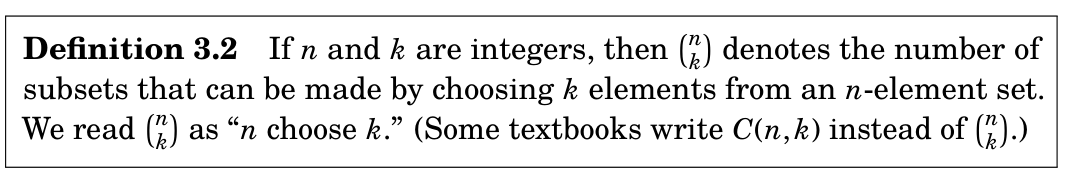
\includegraphics[width=0.9\textwidth]{images/definition03_02.png}
	\label{fig:mypicture}
\end{figure}

\begin{exercise}{}{}
	How many 10-digit binary strings are there that do not have exactly four
	1's?
	\begin{alist}
		\item Let $A=$ set of all 10-digit binary strings.
		\item Let $B=$ set of all 10-digit binary strings with exactly four 1's.
		\item Let $C=$ set of all 10-digit binary strings that do not have exactly
		four 1's.
		\item Because B and C are complements and A is the universe of all 10-digit
		binary strings, then $B \cup C = A$ and $|A|-|B| = |C|$.
		\item Using the multiplication principle, we determine $|A|$ is $2^{10}$.
		\item For $B$, there are 4 spots out of 10 where we can place 1s. Therefore
		\mbox{$|B|=\binom{10}{4}$}.
		\item Therefore $|C|=2^{10} - \binom{10}{4}$.
	\end{alist}
\end{exercise}

\begin{exercise}{}{}
	A = $\{ 0,1,2,3,4,5,6,7,8,9\}$
	\begin{alist}
		\item Let $B=$ Even elements of A.
		\item Let $C=$ Odd elemements of A.
		\item Let $D=$ 6-elements subsets of A that have exactly 3 even elements.
		\item Let $E=$ 6-elements subsets of A that do not have exactly 3 even elements.
		\item How many 6-element subsets of A have exactly three even elements?
		\item We can first choose 3 elements from B, and then choose 3 elements
		of C, and combine them together with the multiplication principle.
		\item $|B| = |C| = \dbinom{5}{3}$, and therefore $|D| = {\dbinom{5}{3}}^2$.
		\item How many do not have exactly three even elements?
		\item E is the complement of D, therefore $|E| = \dbinom{10}{6} -
			{\dbinom{5}{3}}^2$.
	\end{alist}
\end{exercise}

\begin{exercise}{}{}
	Let $A$ be the set of 10-digit binary strings.
	\begin{alist}
		\item Let $B=$ subset of A with exactly four 1's
		\item Let $C=$ subset of A with exactly five 1's
		\item Let $D=$ subset of A whose elements have exactly four 1's or exactly five 1's
		\item Let $E=$ subset of A whose elements do not have exactly four 1's
		or exactly five 1's
		\item How many elements of A are there that have exactly four 1's or exactly five 1's?
		\item Because $B \cap C=\emptyset$, B and C partition D. Therefore, we can
		calculate the cardinalities separately and then add them.
		\item $|B|=\binom{10}{4}$ and $|C|=\binom{10}{5}$, $|D|= \binom{10}{4}+\binom{10}{5}$.
		\item How many do not have exactly four 1's or exactly five 1's?
		\item $E$ is the complemenet of D, therefore $|E| = |A| - |D| = 2^{10} -
			\binom{10}{4}-\binom{10}{5}$.
	\end{alist}
\end{exercise}

\begin{exercise}{}{}
	How many 10-digit binary strings have an even number of 1's?
	\begin{alist}
		\item Let $A$ be the set of 10-digit binary strings.
		\item Let $B=$ subset of A with exactly 0 1's
		\item Let $C=$ subset of A with exactly 2 1's
		\item Let $D=$ subset of A with exactly 4 1's
		\item Let $E=$ subset of A with exactly 6 1's
		\item Let $F=$ subset of A with exactly 8 1's
		\item Let $G=$ subset of A with exactly 10 1's
		\item Let $H=$ subset of A with an even number of 1's
		\item Because B, C, D, E, F, and G partition H, $H=B\cup C\cup D\cup E \cup
			F \cup G$, and therefore $|H|=|B| + |C| + |D| + |E| + |F| + |G|$.
		\item Because of the equivalance of $\binom{n}{k}$ and $\binom{n}{n-k}$,
		$|B|=|G|, |C|=|F|, |D|=|E|$.
		\item Therefore $|H| =
			2\cdot \binom{10}{0} +
			2\cdot \binom{8}{2} +
			2\cdot \binom{6}{4}$.
	\end{alist}
\end{exercise}

\begin{exercise}{}{}
	A 5-card poker hand is called a flush if all cards are the same suit. How
	many different flushes are there?
	\begin{alist}
		\item To get a flush of one particular suit, we choose 5 cards from a set of 13,
		which equals $\dbinom{13}{8}$.
		\item Because there are 4 different suits in the deck of card, we have 4 ways of
		getting the flush and the total number of flush possibilities is $4 \cdot
			\dbinom{13}{8}$.
	\end{alist}
\end{exercise}

\section{Pascal's Triangle and Binomial Theorem}

\begin{definition}{Pascal's Identity\index{Pascal's Identity}}{}
	\begin{align*}
		\binom{n+1}{k}=\binom{n}{k-1}+\binom{n}{k}
	\end{align*}
\end{definition}

\begin{intuition}{Pascal's Identity}{}
	\begin{align*}
		A & =\set{0,1,2,3, \ldots, n}                                                                                     \\
		x & =\binom{n+1}{k}           &  & \text{count of}\;k\;\text{element subsets of}\;A                               \\
		y & =\binom{n}{k-1}           &  & \text{count of subsets of k element subsets}\;A\;\text{which do contain}\;0    \\
		z & =\binom{n}{k}             &  & \text{count of subsets of k element subsets}\;A\;\text{which don't contain}\;0 \\
		z & =x + y
	\end{align*}

	\begin{alist}
		\item For $y$, first reduce $A$ by taking out $0$, and then choose
		subsets of size $k-1$, aka $\binom{n}{k-1}$.  Then for each of those
		subsets union them with the set $\set{0}$. Now we have subsets of size $k$, all of
		them contain 0, and a there is still a total of $\binom{n}{k-1}$.
		\item For $z$, first reduce $A$ by taking out $0$, and then choose
		subsets of size $k$, aka $\binom{n}{k}$.  Now we have subsets of size $k$, all of
		them do not contain 0.
		\item This just states the obvious fact that the number of $k$-element
		subsets of $A$ equals the number of $k$-element subsets that contain
		0 plus the number of $k$-element subsets that do not contain 0 .
	\end{alist}
\end{intuition}

\begin{definition}{Binomial Theorem\index{binomial theorem}}{}
	\begin{align*}
		n       \in \mathbb{N}_{>0} \implies
		(x+y)^n =\binom{n}{0}
		x^n+\binom{n}{1} x^{n-1} y
		+\cdots+\binom{n}{n-1} x y^{n-1}+\binom{n}{n} y^n
	\end{align*}
\end{definition}

\begin{intuition}{Binomial Theorem}{}
	we're choosing either the first or second term in the expression...
	flush me out
\end{intuition}

\begin{intuition}{Subsets to Polynomials}{}
	\begin{alist}
		\item
		\item binomial coefficients count subsets.
		\item When expanding a binomial expression like $(1+x)^n$,
		\item each term corresponds to choosing a subset of size $k$ from a set of size $n$, and
		\item the coefficient of each term is the number of ways to choose that subset,
		\item which is exactly \(\binom{n}{k}\). Thus, the coefficients in the expansion of
		\((1+x)^n\) represent the number of subsets of size \(k\), connecting
		polynomial expansion directly to counting subsets. This relationship is
		fundamental in combinatorics and probability.
	\end{alist}
\end{intuition}

\[
	\begin{array}{cccccccc}
		  &   &   & 1 &   &   &   & \\
		  &   & 1 &   & 1 &   &   & \\
		  & 1 &   & 2 &   & 1 &   & \\
		1 &   & 3 &   & 3 &   & 1 & \\
	\end{array}
\]

\begin{exercise}{}{}
	Write out row 11 of pascal's triangle.
	\begin{alist}
		\item the first 6 terms of row 11 are unique, and the next fiver terms
		are mirrors of the first five.
		\item the terms of row 11 can be calculated with $\dbinom{11}{i}$, where
		$i \in \mathbb{n}, 0 \leq i \leq 11$.
		\item the $1^{st}$ and $11^{th}$ term of row 11 is
		$\dbinom{11}{0}=\dfrac{11!}{11!\cdot0!}=1$.
		\item the $2^{st}$ and $10^{th}$ term of row 11 is
		$\dbinom{11}{1}=\dfrac{11!}{10!\cdot1!}=11$.
		\item the $3^{rd}$ and $9^{th}$ term of row 11 is
		$\dbinom{11}{2}=\dfrac{11!}{9!\cdot2!}=55$.
		\item the $4^{th}$ and $8^{th}$ term of row 11 is
		$\dbinom{11}{3}=\dfrac{11!}{8!\cdot3!}=165$.
		\item the $5^{th}$ and $7^{th}$ term of row 11 is
		$\dbinom{11}{4}=\dfrac{11!}{7!\cdot4!}=330$.
		\item the $6^{th}$ term of row 11 is
		$\dbinom{11}{5}=\dfrac{11!}{5!\cdot6!}=462$.
	\end{alist}
\end{exercise}

\begin{exercise}{}{}
	Use the binomial theorem to find the coefficient of $x^8 y^5$
	in $(x+ y)^{13}$.
	\begin{alist}
		\item $\dbinom{13}{8}=\dfrac{13!}{8!\cdot5!}\approx 10,00$
	\end{alist}
\end{exercise}

\begin{exercise}{}{}
	Use the binomial theorem to find the coefficient of $x^8$
	in $(x+2)^{13}$.
	\begin{alist}
		\item Let $a=2$, and then $x+2=x+a$
		\item The coefficient of $x^8a^5$ is $\binom{13}{8}$, therefore the coefficient
		of $x^8$ is $2^5\cdot\binom{13}{8}=32\cdot\binom{13}{8}$.
	\end{alist}
\end{exercise}

\begin{exercise}{}{}
	Use the binomial theorem to find the coefficient of $x^6y^3$
	in $(3x-2y)^9$.
	\begin{alist}
		\item Let $a=3x, b=-2y$, and the coefficient for $a^6b^3$ from $(a+b)^9$
		is $\binom{9}{6}$.
		\item Therefore the coeffecient for $x^6y^3$ in $(3x-2y)^9$ is
		$3^6\cdot(-2)^3\cdot\binom{9}{6}$.
	\end{alist}
\end{exercise}

\begin{exercise}{}{}
	Use the binomial theorem to show $\sum\limits_{k=0}^n\binom{n}{k}=2^n$.
	\begin{alist}
		\item The binomial theorem states
		$$(x+y)^n=\sum\limits_{i=0}^n\dbinom{n}{i}x^{n-i}y^i$$
		\item Let $x=y=1$, therefore
		$$2^n=\sum\limits_{i=0}^n\dbinom{n}{i}1^{n-i}1^i$$
		$$2^n=\sum\limits_{i=0}^n\dbinom{n}{i}$$
	\end{alist}
\end{exercise}

\begin{exercise}{}{}
	Use Definition 3.2 and Fact 1.3 to show $\sum\limits_{k=0}^n\binom{n}{k}=2^n$.
	\begin{alist}
		\item Suppose there exists some set A, where $|A|=n$.
		\item Now let us suppose some set $A_i$, where $i\in \mathbb{N}, 0\leq i
			\leq n$, where $A_i$ represents a subset of $A$ with cardinality $i$.
		\item The number of unique subsets $A_i$ is given by $\binom{n}{i}$, as
		provided in Definition 3.2.
		\item The number of all unique subsets $A_i, i=0\ldots n$ is given by
		$\sum\limits_{i=0}^n\binom{n}{i}$.
		\item All unique subsets $A_i$ is another name for the powerset $\mathbb{P}(a)$,
		and the cardinality of $\mathbb{P}(a)=2^n$, as provided in Fact 1.3.
		\item Therefore $\sum\limits_{k=0}^n\binom{n}{k}=2^n$.
	\end{alist}
\end{exercise}

\begin{exercise}{}{}
	Use the binomial theorem to show the following.
	\begin{alist}
		\item
		$$\sum\limits_{k=0}^n 3^k \binom{n}{k}=4^n$$
		\item
		The binomial theorem asserts the following.
		$$
			(x+y)^n = \sum\limits_{k=0}^n \dbinom{n}{k} x^{n-k}y^k
		$$
		\item Let $x=1, y=3$, then
		$$
			(1+3)^n = \sum\limits_{k=0}^n \dbinom{n}{k} 1^{n-k}3^k
		$$
		$$
			4^n = \sum\limits_{k=0}^n \dbinom{n}{k} 3^k
		$$
	\end{alist}
\end{exercise}


\begin{exercise}{}{}
	Use Fact 3.5 (page 87) to derive Equation 3.3 (page 90).
	\begin{alist}
		\item First let's expand out the right hand side, and get a common denominator.
		$$\dbinom{n}{k-1} =\dfrac{n!}{(k-1)!(n-k+1)!}$$
		$$=\dfrac{n!}{(k-1)!(n-k)!(n-k+1)} =\dfrac{kn!}{k(k-1)!(n-k)!(n-k+1)}$$

		$$\dbinom{n}{k}=\dfrac{n!}{k!(n-k)!}=
			\dfrac{n!}{k(k-1)!(n-k)!}=
			\dfrac{(n-k+1)n!}{(n-k+1)k(k-1)!(n-k)!}
		$$

		$$\dbinom{n}{k-1} + \dbinom{n}{k}=$$
		$$ \dfrac{kn!+(n-k+1)n!}{(n-k+1)k(k-1)!(n-k)!}=
			\dfrac{n!(k+n-k+1)}{(n-k+1)!k!}= $$
		$$ \dfrac{n!(n+1)}{(n-k+1)!k!}=
			\dfrac{(n+1)!}{(n-k+1)!k!}= \dbinom{n+1}{k}$$
	\end{alist}
\end{exercise}

\begin{exercise}{}{}
	Use the binomial theorem to show
	\begin{alist}
		\item
		$$
			\dbinom{n}{0}
			- \dbinom{n}{1}
			+ \dbinom{n}{2}
			- \dbinom{n}{3}
			+ \dbinom{n}{4}
			\dots
			+ (-1)^n\dbinom{n}{n} =0, \quad n>0.
		$$
		\item The binomial theorem states
		$$(x+y)^n=\sum\limits_{i=0}^n\dbinom{n}{i}x^{n-i}y^i$$
		$$
			\dbinom{n}{0}
			- \dbinom{n}{1}
			+ \dbinom{n}{2}
			- \dbinom{n}{3}
			+ \dbinom{n}{4}
			\dots
			+ (-1)^n\dbinom{n}{n}=(1+(-1))^n = 0^n = 0
		$$
	\end{alist}
\end{exercise}

\begin{exercise}{}{}
	Show that the formula $k\dbinom{n}{k}=n\dbinom{n-1}
		k-1$
	is true for all integers $n, k$ with $0 \leq k \leq n$.
	\begin{alist}
		\item Suppose $k\neq0$
		$$k\dbinom{n}{k}=n\dbinom{n-1}{k-1}$$
		$$k\dfrac{n!}{(n-k)!k!}=n\dfrac{(n-1)!}{(k-1)!(n-1-k+1)!}$$
		$$k\dfrac{n!}{(n-k)!k!}=\dfrac{n!}{(k-1)!(n-k)!}$$
		$$k\dfrac{n!}{(n-k)!k!}=\dfrac{n!}{(k-1)!(n-k)!}\cdot\dfrac{k}{k}$$
		$$k\dfrac{n!}{(n-k)!k!}=k\dfrac{n!}{(n-k)!k!}$$
		\item Suppose $k=0$
		$$0\cdot\dbinom{n}{0}=n\dbinom{n-1}{-1}$$
		$$0\cdot\dbinom{n}{0}=n\cdot 0$$
		$$0=0$$
	\end{alist}
\end{exercise}

\begin{exercise}{}{}
	Use the binomial theorem to show
	\begin{alist}
		\item
		$$9^n=\sum\limits_{k=0}^{n} (-1)^k\dbinom{n}{k}10^{n-k}$$
		\item The binomial theorem states
		$$(x+y)^n=\sum\limits_{i=0}^n\dbinom{n}{i}x^{n-i}y^i$$
		\item let $x=-1, y=10$
		$$((-1)+10)^n=\sum\limits_{k=0}^{n} (-1)^k\dbinom{n}{k}10^{n-k}$$
	\end{alist}
\end{exercise}

\begin{exercise}{}{}
	Show that
	$$
		\dbinom{n}{k}
		\dbinom{k}{m}=
		\dbinom{n}{m}
		\dbinom{n-m}{k-m}
	$$
	\begin{alist}
		\item
		$$
			\dbinom{n}{k}
			\dbinom{k}{m}=
			\dfrac{n!}{(n-k)!k!}
			\dfrac{k!}{(m-k)!m!}=
			\dfrac{n!}{(n-k)!(m-k)!m!}
		$$
		$$
			\dbinom{n}{m}
			\dbinom{n-m}{k-m}=
			\dfrac{n!}{(n-m)!m!}\cdot
			\dfrac{(n-m)!}{(k-m)!(n-m-k+m)!}=
		$$
		$$
			\dfrac{n!}{m!}\cdot
			\dfrac{1}{(k-m)!(n-k)!}=\dfrac{n!}{(n-k)!(m-k)!m!}
		$$
	\end{alist}
\end{exercise}

\begin{exercise}{}{}
	Show that
	\begin{alist}
		\item
		$$
			\dbinom{n}{3}=
			\dbinom{2}{2} +
			\dbinom{3}{2} +
			\dbinom{4}{2} +
			\dbinom{5}{2} +
			\dots +
			\dbinom{n-1}{2}
		$$

		\item Remember this equality:
		$$\dbinom{n+1}{k} = \dbinom{n}{k} + \dbinom{n}{k-1}$$

		\item The binomial theorem states
		$$(x+y)^n=\sum\limits_{i=0}^n\dbinom{n}{i}x^{n-i}y^i$$
		\item

		\item Suppose $k=3$
		$$
			\dbinom{n}{3}=
			\dbinom{n-1}{2} +
			\dbinom{n-1}{3}
		$$
		$$
			\dbinom{n-1}{3} =
			\dbinom{n-2}{2} +
			\dbinom{n-2}{3}
		$$
		$$
			\dbinom{n-2}{3} =
			\dbinom{n-3}{2} +
			\dbinom{n-3}{3}
		$$
		$$
			\dots
		$$
	\end{alist}
\end{exercise}
\begin{figure}
	\centering
	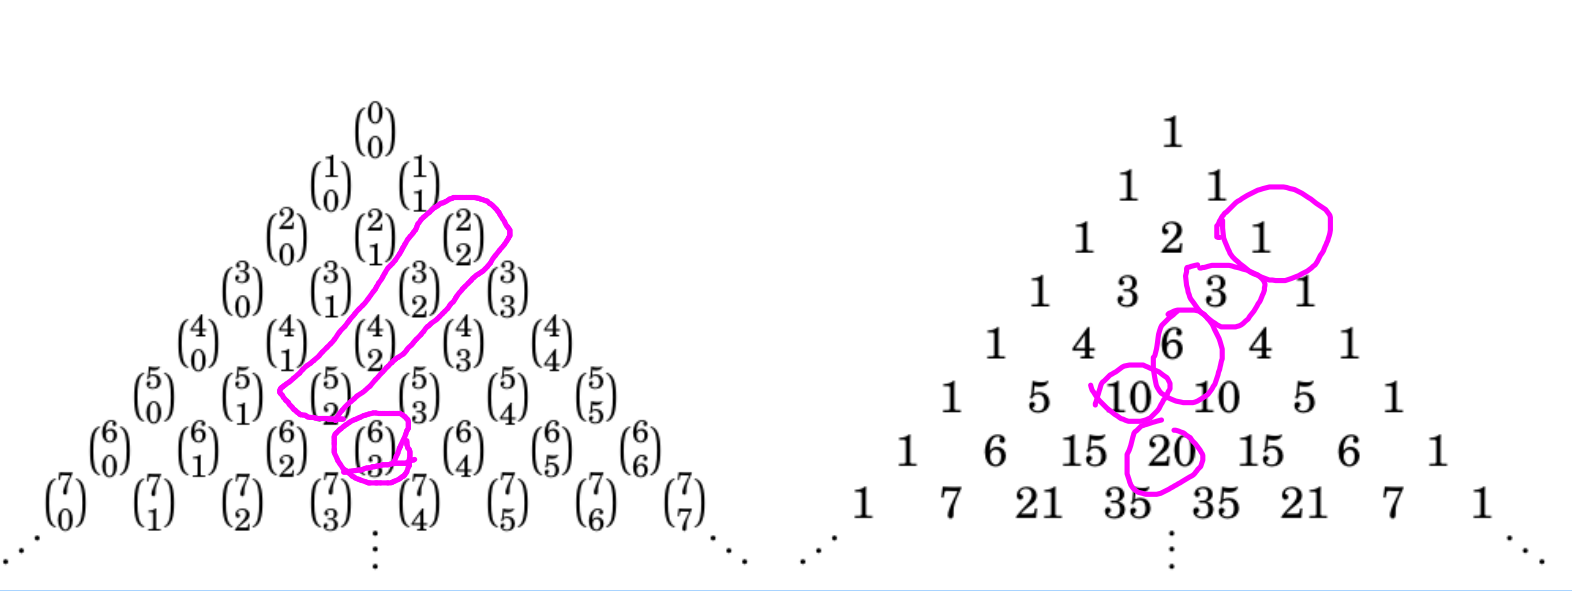
\includegraphics[width=0.7\textwidth]{images/pascals-triangle.png}
\end{figure}
\begin{exercise}{}{}
	The first five rows of Pascal's triangle appear in the digits of powers of 11: 110 = 1,
	111 = 11, 112 = 121, 113 = 1331 and 114 = 14641. Why is this so? Why does the
	pattern not continue with 115?
\end{exercise}

\section{Inclusion Exclusion}

\begin{definition}{Inclusion-Exclusion Formula\index{inclusion-exclusion formula}}{}
	If $A$ and $B$ are finite sets, then $|A \cup B|=|A|+|B|-|A \cap B|$.
\end{definition}

\begin{exercise}{}
	At a certain university 523 of the seniors are history
	majors or math majors (or both). There are 100 senior math majors, and 33
	seniors are majoring in both history and math. How many seniors are majoring in
	history?
	\begin{alist}
		\item Let $A=$ math majors, $|A|=100$
		\item Let $B=$ history majors
		\item $A\cap B=$ both history and math major, $|A\cap B|=33$
		\item $A \cup B$ =math or history majors or both, $|A\cup B|=|A| +
			|B| - |A\cap B|=523$
		\item
		$$|A\cup B|=|A| + |B| - |A\cap B|=523$$
		$$|B| = 523 + |A\cap B| - |A|$$
		$$|B| = 523 + 33 - 100$$
		$$|B| = 456$$
	\end{alist}
\end{exercise}

\begin{exercise}{}{}
	How many 4-digit positive integers are there for which
	there are no repeated digits, or for which there may be repeated digits, but
	all digits are odd?
	\begin{alist}
		\item Let $A=$ 4-digit positive integers
		\item Let $B=$ 4-digit positive integers with no repeated digits, $B \subset
			A$
		\item Let $C=$ 4-digit positive integers with repeated digits and all digits
		are odd, $C \subset A$
		\item $C\cap B$  = 4-digit positive integers for which there are
		no repeated digits and all digits are odd.
		\item $C\cup B$  = 4-digit positive integers for which there are
		no repeated digits, or for which there may be repeated digits, but all
		digits are odd.
		\item
		$$|C\cup B| = |C| + |B| - |C\cap B|$$
		\item For B, we can pick any number 1..9 to start, and then for each
		subsequent digit we can pick between 0..9, excluding the one that came
		before, therefore there are also 9 choices for each non-starting digit.
		$|B| = 9^4$.
		\item For C, we can pick any number 1,3,5,7,9 for all 4 positions, therefore
		$|C|=5^4$.
		\item For $|C\cap B|$, we can pick any number 1,3,5,7,9 for the first
		position, and thereafter we can pick from any of the odd digits that did
		not directly precede the current one, therefore there are $|C \cap
			B|=5\cdot4^3$.
		\item $$|C\cup B| = |C| + |B| - |C\cap B|$$
		\item $$|C\cup B| = 5^4+9^4-5\cdot 4^3$$
	\end{alist}
\end{exercise}

\begin{exercise}{}{}
	How many 4-digit positive integers are there that are even or contain no 0's?
	\begin{alist}
		\item Let $A=$ 4-digit positive integers that are even
		\item Let $B=$ 4-digit positive integers that contain no zeros
		\item $A \cap B=$ 4-digit positive integers that are even and contain no zeros
		\item $A \cup B=$ 4-digit positive integers that are even or contain no zeros
		\item To create elements in A, we can pick 1..9 to start, then 0..9 for the
		second and third digits, and any of the 5 even digits for the last
		digit, therefore $|A|=9\cdot 10^2\cdot5$.
		\item To create elements in B, we can pick from 1..9 for all digits,
		therefore $|B|=9^4$.
		\item To create elements in $A\cap B$, we can pick from 1..9 for the first
		3 digits and 2,4,6,8 for the last digit, therefore $|A\cap B|=9^3\cdot4$
		\item $$|A\cup B| = |A| + |B| - |A\cap B|$$
		\item $$|A\cup B| = 9\cdot10^2\cdot5 + 9^4 - 9^3\cdot4$$
	\end{alist}
\end{exercise}

\begin{exercise}{}{}
	This problem involves lists made from the letters T, H, E, O, R, Y, with repetition allowed.
	\begin{alist}
		\item (a) How many 4-letter lists are there that don't begin with T, or don't
		end in Y?
		\item Let $A=$ 4-letter lists that dont begin with T
		\item Let $B=$ 4-letter lists that dont end with Y
		\item Let $A\cap B=$ 4-letter lists that dont begin with T and dont end with Y
		\item Let $A\cup B=$ 4-letter lists that dont begin with T or dont end with Y
		\item $|A|= 5\cdot6\cdot6\cdot6$
		\item $|B|= 6\cdot6\cdot6\cdot5$
		\item $|A\cap B|= 5\cdot6\cdot6\cdot5$
		\item $|A\cup B|= |A| + |B| - |A\cap B| = 2\cdot 6^3\cdot5 - 5^2\cdot6^2$
		\item (b) How many 4-letter lists are there in which the sequence of letters T,
		H, E appears consecutively (in that order)?
		\item Other than THE, there is one letter-spot left free, and there are 6 letters
		available for that spot. THE can be placed starting at either position 1 or
		position 2 for a total of two choices. Therefore by the multiplication
		principle there are $2\cdot6$ 4-letter lists matching the problem criteria.
		\item (c) How many 6-letter lists are there in which the sequence of letters T,
		H, E appears consecutively (in that order)?
		\item Other than THE, there are three letter-spots left free, and there are 6 letters
		available for those 3 spots. THE can be placed starting at either position
		1, 2, 3, or 4 for a total of four choices. Therefore by the multiplication
		principle there are $4\cdot6^3$ 6-letter lists matching the problem criteria.
	\end{alist}
\end{exercise}

\begin{exercise}{}{}
	How many 7-digit binary strings begin in 1 or end in 1 or have exactly four 1's?
	\begin{alist}
		\item Let $A=$ 7-digit binary strings that begin in 1
		\item Let $B=$ 7-digit binary strings that end in 1
		\item Let $C=$ 7-digit binary strings that have exactly four 1s
		\item Let $D=$ 7-digit binary strings
		\item $A\cup B \cup C=$ 7-digit binary strings begin in 1 or end in 1 or have exactly four 1's
		\item $\neg(A\cup B \cup C)=\neg A \cap \neg B \cap \neg C=$
		7-digit binary strings dont begin in 1 and dont end in 1 and dont have
		exactly four 1's.
		\item To create elements of $\neg A \cap \neg B \cap \neg C$,
		the first and last digit must be 0. For the middle 5 spots, there must
		be either 0, 1, 2, 3, or 5 1s. This means there are
		$\binom{5}{0}+\binom{5}{1}+\binom{5}{2}+\binom{5}{3}+\binom{5}{5}$ ways
		to arrange the middle 5 spots.
		\item We can use the fact that $A\cup B \cup C$ is the complement of
		$\neg(A\cup B \cup C)$ to determine that
		$$|D| - |\neg(A\cup B \cup C)|=| A\cup B \cup C |$$
		$$ | A\cup B \cup C | = 2^7 - \binom{5}{0}-\binom{5}{1}-\binom{5}{2}-\binom{5}{3}-\binom{5}{5}$$
	\end{alist}
\end{exercise}

\begin{exercise}{}{}
	Is the following statement true or false? Explain. If
	$A_1
		\cap A_2 \cap A_3 =\emptyset$ , then $|A_1 \cup A_2 \cup A_3| =
		|A_1|+|A_2|+|A_3|$.

	\begin{alist}
		\item
		$$
			A_1 \cap A_2 \cap A_3 =\emptyset
			\implies
			|A_1 \cup A_2 \cup A_3| = |A_1|+|A_2|+|A_3|
		$$
		\item Suppose $A_1 \cap A_2 \cap A_3 =\emptyset$.
		\item Let
		$A_1=\{1, 2\},\quad
			A_2=\{1, 3\},\quad
			A_3=\{4, 5\} $
		\item This is a counter-example as $|A_1 \cup A_2 \cup A_3|=5$ while
		$|A_1|+|A_2|+|A_3| = 2 +2 +2=6$.
		\item For the implication to hold, we must also know that intersection between
		any two of the sets is also the empty-set.
	\end{alist}
\end{exercise}

\begin{exercise}{}{}7. Consider 4-card hands dealt off of a standard 52-card deck.
	How many hands are there for which all 4 cards are of the same suit or all 4
	cards are red?
	\begin{alist}
		\item Let $A=$ all 4 cards are the same suit
		\item Let $B=$ all 4 cards are red
		\item $A\cap B=$ all 4 cards are same suit AND all 4 cards are red
		\item $A\cup B=$ all 4 cards are same suit OR all 4 cards are red
		\item
		$$
			|A \cup B | = |A| + |B| - |A \cap B|
		$$
		\item $|A| = 4\cdot\dbinom{13}{4}$
		\item $|B| = \dbinom{26}{4}$
		\item $|A\cap B| = 2\cdot\dbinom{13}{4}$
		\item
		$$
			|A \cup B | = 4\cdot\dbinom{13}{4} + \dbinom{26}{4} - 2\cdot\dbinom{13}{4}
		$$
	\end{alist}
\end{exercise}

\begin{exercise}{}{}
	Consider 4-card hands dealt off of a standard 52-card deck.
	How many hands are there for which all 4 cards are of different suits or all
	4 cards are red?
	\begin{alist}
		\item Let $A=$ all 4 cards are of different suit
		\item Let $B=$ all 4 cards are red
		\item $A\cap B=\emptyset$ all 4 cards are different suit and all 4 cards are red
		\item $|A| = \dfrac{13^4}{4!}$
		\item $|B| = \dbinom{26}{4}$
		\item
		$$
			|A \cup B | = |A| + |B| - |A \cap B|
			|A \cup B | = \dfrac{13^4}{4!} + \dbinom{26}{4} - 0
		$$
	\end{alist}
\end{exercise}

\begin{exercise}{}{}
	A 4-letter list is made from the letters L, I, S, T, E, D
	according to the following rule: Repetition is allowed, and the first two
	letters on the list are vowels or the list ends in D. How many such lists are
	possible?
	\begin{alist}
		\item Let $A=$ first two letters on the list are vowels
		\item Let $B=$ the list ends in D
		\item $A\cap B=$ first two letters on the list are vowels and the list ends in D
		\item $A\cup B=$ first two letters on the list are vowels or the list ends in D
		\item To determine $|A|$, we note that there are $2^2$ to pick the first two
		letters as vowels, and then $6^4$ possibilities for the next four letters.
		\item To determine $|B|$, the last letter is fixed, and there $6^5$
		possibilities for the first 5 letters.
		\item To determine $|A\cap B|$ there are $2^2$ possibilities for the first two
		letters as vowel, the last letter is fixed, and the middle 3 letters have
		$6^3$ possible arrangements.
		\item Therefore
		$$|A \cup B | = |A| + |B| - |A \cap B|$$
		$$|A \cup B | = 2^2\cdot6^4 + 6^5 - 2^2\cdot6^3$$
	\end{alist}
\end{exercise}

\begin{exercise}{}{}
	How many 6-digit numbers are even or are divisible by 5?
	\begin{alist}
		\item let $a=$ 6-digit numbers that are even
		\item let $b=$ 6-digit numbers that are divisible by 5
		\item $a\cap b=$ 6-digit numbers that are even and divisible by 5
		\item $a\cup b=$ 6-digit numbers that are even or divisible by 5
		\item $|a|=9\cdot10^4\cdot5$
		\item $|b|=9\cdot10^4\cdot2$
		\item $|a\cap b|= 9\cdot10^4\cdot1$
		\item $$|a\cup b|= 9\cdot10^4\cdot5 + 9\cdot10^4\cdot2 - 9\cdot10^4\cdot1$$
		\item $$= (9\cdot10^4)(5 + 2 -1)$$
		\item $$= 54\cdot10^4$$
	\end{alist}
\end{exercise}

\begin{exercise}{}{}
	How many 7-digit numbers are even or have exactly three digits equal to 0?
	\begin{alist}
		\item let $a=$ 7-digit numbers that are even
		\item let $b=$ 7-digit numbers that have exactly three digits equal to 0
		\item $a\cap b=$ 7-digit numbers that are even and have exactly three digits equal to 0
		\item $a\cup b=$ 7-digit numbers that are even or have exactly three digits equal to 0
		\item $|a|=9\cdot10^6\cdot5$
		\item to calculate $|b|$, we note that there must be three 0s, and because we
		can't start the number with 0, there are $\dbinom{6}{3}$ possible choices of
		where to place them. for the remaining 4 digits, there are
		9 choices for the first digit and $10^3$ for the remaining choices. then by the multiplication principle, there are
		$|b|=9\cdot10^3\cdot \dbinom{6}{3}$.
		\item to calculate $|a\cap b|$, we consider two different cases. in the first
		case, the number ends with 0, therefore there are two zeros to place in 5
		spots. the first digit has 9 choices, the non-zeroes have $10^3$ choices,
		and so $9\cdot\dbinom{5}{2}\cdot10^3$. possibilties for this case. for the
		second case that does not end with a zero, there are 9 choices for the
		first digit, $\dbinom{5}{3}$ for the zeros, and 4 choices for the last
		digit, and $10^2$ for the remaining digits. therefore there are
		$9\cdot\dbinom{5}{3}\cdot10^2\cdot4$ for the second case. the cases sum together for
		$9\cdot\dbinom{5}{3}\cdot10^2\cdot4 +
			9\cdot\dbinom{5}{2}\cdot10^3$ total choices from $|a\cap b|$.
		\item therefore
		$$|a \cup b | = |a| + |b| - |a \cap b|$$
		$$|a \cup b | =
			9\cdot10^6\cdot5 + 9\cdot10^3\cdot \dbinom{6}{3} - 9\cdot\dbinom{5}{3}\cdot10^2\cdot4 - 9\cdot\dbinom{5}{2}\cdot10^3$$
	\end{alist}
\end{exercise}

\begin{exercise}{}{}
	12. How many 5-digit numbers are there in which three of the
	digits are 7, or two of the digits are 2?
	\begin{alist}
		\item Let $A=$ 5-digit numbers in which at least three of the digits are 7
		\item Let $B=$ 5-digit numbers in which at least two of the digits are 2
		\item $A\cap B= $ 5-digit numbers in which two of the digits are 2 AND three are 7
		\item $A\cup B= $ 5-digit numbers in which two of the digits are 2 OR three are 7

		\begin{itemize}
			\item 5 7s = If there are 5 7's, there is only way to create that digit. $1$
			\item 4 7s = If there are 4 7's, there are 8 ways to create that digit if
			      the number does not start with 7, and $\dbinom{4}{3}\cdot9$ ways if it
			      does start with 7.
			\item 3 7s = If there are 4 7's, there are 8 ways to create that digit if
			      the number does not start with 7, and $\dbinom{4}{3}\cdot9$ ways if it
			      does start with 7.
		\end{itemize}

		\item $|A|$, case 1, where it begins with 7. Then the remaining 7s can go in
		$\dbinom{4}{2}$ spots, and the remaining two digits have $9^2$ choices.
		\item $|A|$, case 1, where it does not begin with 7. There are 8 choices for the
		first digit (exclude 0 and 7), $\dbinom{4}{3}$ spots for the 7s, and 9 spots
		for the remaining digit.

		\item didnt finish. These problems are becoming a grind ...
	\end{alist}
\end{exercise}

% % 13. How many 8-digit binary strings end in 1 or have exactly four 1's?
% % 14. How many 3-card hands (from a standard 52-card deck) have the property that
% % it is not the case that all cards are black or all cards are of the same suit?
% % 15. How many 10-digit binary strings begin in 1 or end in 1?

\section{Counting Multisets}

\begin{definition}{Stars and Bars}{}
	We can encode the multisets as lists made from the two symbols $*$ and $|$,
	with an $*$ for each element of the multiset, as follows.
\end{definition}

\begin{definition}{}{}
	The number of $k$-element multisets that can be made from the elements of an
	$n$-element set $X=\left\{x_1, x_2, \ldots, x_n\right\}$ is

	\begin{align*}
		\binom{k+n-1}{k}=\binom{k+n-1}{n-1} .
	\end{align*}

	This works because any cardinality-$k$ multiset made from the $n$ elements
	of $X$ can be encoded in a star-and-bar list of length $k+n-1$, having form
	with $k$ stars and $n-1$ bars separating the $n$ groupings of stars. Such a
	list can be made by selecting $n-1$ positions for the bars, and filling the
	remaining positions with stars, and there are $\binom{k+n-1}{n-1}$ ways to
	do this.
\end{definition}

\begin{definition}{Multiset Permutation}{}
	Suppose a multiset $A$ has $n$ elements, with multiplicities $p_1, p_2,
		\ldots, p_k$. Then the total number of permutations of $A$ is

	\begin{align*}
		\frac{n!}{p_{1}!p_{2}!\cdots p_{k}!}
	\end{align*}
\end{definition}


\begin{exercise}{}{}
	How many 10-element multisets can be made from the symbols $\set{1,2,3,4}$?
	\begin{alist}
		\item Let $X= \{ 1,2,3,4\}$, and $|X|=4$.
		\item Let $Y=$ a multiset of cardinality 10.
		\item The total permutations of a k-multiset constructed from a set with
		n-cardinality is
		$$ \dbinom{k+n-1}{k} = \dbinom{k+n-1}{n-1} $$
		\item For this problem $k=10, n=4$.
		\item Therefore there are $\binom{13}{4}$ possible 10-element multisets made
		from the symbols $1\dots4$.
	\end{alist}
\end{exercise}

\begin{exercise}{}{}
	2. How many 2-element multisets can be made from the 26 letters of the alphabet?
	\begin{alist}
		\item Let $A=$ 26 letter alphabet.
		\item Let $Y=$ a multiset of cardinality 2.
		\item For this problem, $k=2, n=26$
		$$ \dbinom{k+n-1}{k} = \dbinom{k+n-1}{n-1} $$
		$$ \dbinom{27}{2}$$
		$$ \dfrac{27!}{25!\cdot2!}$$
		$$ \dfrac{26\cdot27}{2}$$
	\end{alist}
\end{exercise}

\begin{exercise}{}{}
	You have a dollar in pennies, a dollar in nickels, a dollar in dimes, and a dollar in quarters. You give a friend four coins. How many ways can this be done?
	\begin{alist}
		\item Let the set $A= \{a_1, a_2, a_3, a_4\}$, where $a_i$ is a coin type.
		\item The question is equivalent to: given a set of cardinality 4, how many
		different multisets of cardinality 4 can be created?
		\item The information about the different number of starting coins is
		irrelevant other than assuring there are at least $k=4$ of each coin.
		\item Therefore the answer is the following
		$$ \dbinom{k+n-1}{k} $$
		$$ \dbinom{7}{4}$$
	\end{alist}
\end{exercise}

\begin{exercise}{}{}
	A bag contains 20 identical red balls, 20 identical blue
	balls, 20 identical green balls, and 20 identical white balls. You reach in
	and grab 15 balls. How many different outcomes are possible?
	\begin{alist}
		\item This question is asking about how many multisets can be created from
		an initial set. Let $a_i$ be the number of starting balls for color $i$.
		Let $k$ be the cardinality of the desired multiset. As long as $a_i\geq k$,
		then all possible multisets can be created.
		\item Therefore the answer is the following
		$$ \dbinom{k+n-1}{k} $$
		$$ \dbinom{15+4-1}{15}$$
		$$ \dbinom{18}{15}$$
	\end{alist}
\end{exercise}

\begin{exercise}{}{}
	A bag contains 20 identical red balls, 20 identical blue balls, 20 identical
	green balls, and one white ball. You reach in and grab 15 balls. How many
	different outcomes are possible?
	\begin{alist}
		\item Let $A$=multiset of 15 of colored balls, from 3 colors
		\item Let $B$=multiset of 14 of colored balls, from 3 colors
		\item Let $C$=multisets of 15 of colored balls starting from 20
		identical red balls, 20 identical blue balls, 20 identical green balls, and
		one white ball.
		\item We can partition $C$ into two sets: those with a white ball and those
		without a white ball. For the first partition, it is the same as asking how
		many multisets of cardinality 14 can be created from a set of 3 balls, which
		is represented by $B$. The second partition is the same as asking how many
		multisets of size 15 can be created from a set of 3 balls, which is
		represented by $A$.
		\item Therefore $C=A \cup B$, and $|C| = |A| + |B|$.
		\item
		$$ |A| = \dbinom{k+n-1}{k} = \dbinom{15+3-1}{15}=\dbinom{17}{15}$$
		$$ |B| = \dbinom{k+n-1}{k} = \dbinom{14+3-1}{14}=\dbinom{16}{14}$$
		$$ |C| = 256 $$
	\end{alist}
\end{exercise}

\begin{exercise}{}{}A bag contains 20 identical red balls, 20 identical blue
	balls, 20 identical green balls, one white ball, and one black ball. You
	reach in and grab 20 balls. How many different outcomes are possible?
	\begin{alist}
		\item Case 1, 0 white balls, 0 black balls, $k=20, n=3$
		$$ \dbinom{k+n-1}{k} = \dbinom{20+3-1}{20}=\dbinom{22}{20}$$
		\item Case 2, 0 white balls, 1 black ball , $k=19, n=3$
		$$ \dbinom{k+n-1}{k} = \dbinom{19+3-1}{19}=\dbinom{21}{19}$$
		\item Case 3, 1 white ball, 0 black balls, $k=19, n=3$
		$$ \dbinom{k+n-1}{k} = \dbinom{19+3-1}{19}=\dbinom{21}{19}$$
		\item Case 4, 1 white ball, 1 black ball, $k=18, n=3$
		$$ \dbinom{k+n-1}{k} = \dbinom{18+3-1}{18}=\dbinom{20}{18}$$
		\item Therefore the answer is
		$$ \dbinom{22}{20} +\dbinom{21}{19} +\dbinom{21}{19} +\dbinom{20}{18}$$
	\end{alist}
\end{exercise}

\begin{exercise}{}{}
	In how many ways can you place 20 identical balls into five
	different boxes?
	\begin{alist}
		\item This is a stars-and-bars type problem, which is the equivalent of asking,
		given a finite set X with cardinality $n$, how many multisets of cardinality
		$k$ can be created? Here the cardinality of X is 5, and k=20.
		\item Therefore the answer is
		$$ \dbinom{k+n-1}{k} = \dbinom{20+5-1}{20}=\dbinom{24}{20}$$
	\end{alist}
\end{exercise}

\begin{exercise}{}{}
	How many lists (x, y, z) of three integers are there with
	$0 \leq x \leq y \leq z \leq 100$?
	\begin{alist}
		\item  Imagine 100 stars, and then placing 2 bars somewhere within them. This
		transforms the problems into asking how many multisets of cardinality 100
		can be created from a set of cardinality 3, which is solved by the
		following.
		$$ \dbinom{100+3-1}{100} = \dbinom{102}{100}$$
	\end{alist}
\end{exercise}

\begin{exercise}{}{}
	A bag contains 50 pennies, 50 nickels, 50 dimes and 50 quarters. You reach
	in and grab 30 coins. How many different outcomes are possible?
	\begin{alist}
		\item Let $p_i$ be the count of count $i$. There are sufficient coins such that
		$\forall i, p_i\geq k$, where $k$ is the cardinality of the desired
		multiset.
		\item There there are this many possible outcomes, where $n$ is the cardinality
		of the distinct coin set.
		$$ \dbinom{k+n-1}{k} = \dbinom{4+30-1}{30}=\dbinom{33}{30}$$
	\end{alist}
\end{exercise}

\begin{exercise}{}{}
	How many non-negative integer solutions does $$u + v+ w+ x+
		y+ z = 90$$ have?
	\begin{alist}
		\item Suppose a set of 90 stars.  We can partition those stars 6 times with 5
		bars, and then we will have transformed the original problem into an
		equivalent formulation stated as: how many multisets of cardinality 90 can
		be created from an initial set of cardinality 6, which is calculated as
		follows.
		$$ \dbinom{90+6-1}{90} = \dbinom{95}{90}$$
	\end{alist}
\end{exercise}

\begin{exercise}{}{}
	How many integer solutions does the equation
	$w + x + y+ z = 100$ have if $w \geq 4, x \geq 2, y \geq 0, z \geq 0$?
	\begin{alist}
		\item Let A = solutions to the problem
		$$w + x + y+ z = 100, w \geq 0, x \geq 0, y \geq 0, z \geq 0$$.
		\item Let $B=w<4$ and $C=x<2$. From the set $|A|$, we must delete all solutions
		where $B\lor C$. So we are left with determining the cardinality of the
		solution set $B \lor C$, which is equal to
		$$
			|B\lor C| = |B| + |C| - |B\land C|
		$$
		\item To determine $|B|$ solve this problem
		$$w + x + y+ z = 100, \neg(w \geq 4), x \geq 0, y \geq 0, z \geq 0$$
		$$\implies x + y+ z = 97, x \geq 0, y \geq 0, z \geq 0$$

		\item To determine $|C|$ solve this problem
		$$w + x + y+ z = 100, w \geq 0, \neg(x \geq 2), y \geq 0, z \geq 0$$
		$$\implies w + y+ z = 99, w \geq 0, y \geq 0, z \geq 0$$

		\item To determine $|B\land C|$ solve this problem
		(w, x)
		(0, 0)
		(0, 1)
		(1, 0)
		(1, 1)
		(2, 0)
		(2, 1)
		(3, 0)
		(3, 1)
		\item There's a much simpler approach.
	\end{alist}
\end{exercise}

\begin{exercise}{}{}
	How many integer solutions does the equation
	$$w + x + y+ z = 100, w \geq 7, x \geq 0, y \geq 5, z \geq 4$$
	\begin{alist}
		\item This problem is the same as
		$$w + x + y+ z = 84, w \geq 0, x \geq 0, y \geq 0, z \geq 0$$
		\item Therefore the solution is calculated with $k=84, n=4$ as
		$$ \dbinom{k+n-1}{k} = \dbinom{84+4-1}{84}=\dbinom{87}{84}$$
	\end{alist}
\end{exercise}

\begin{exercise}{}{}
	How many length-6 lists can be made from the symbols $\{a,
		b, c, d, e, f, g\}$, if repetition is allowed and the list is in
	alphabetical order? (Examples: bbcegg, but not bbbagg.)
	\begin{alist}
		\item Creating lists is equivalent to counting permutations. Only allowing lists
		in some order is equivalent to counting multisets. Therefore this problem
		can be restated in an equivalent form as---how many cardinality 6 multisets
		can be created from an original set of cardinality 7.
		\item This can be calculated as the following, with $k=6, n=7$.
		$$ \dbinom{k+n-1}{k} = \dbinom{6+7-1}{6}=\dbinom{12}{6}$$
	\end{alist}
\end{exercise}

\begin{exercise}{}{}
	How many permutations are there of the letters in the word ``PEPPERMINT''?
	\begin{alist}
		\item This problem is the equivalent to asking---given a multiset, how many
		permutations can be made.  We must know the cardinality of the multiset, and each
		the multiplicity of each element from the underlying set.
		\item Then the permutation can be calculated as follows
		$$ \dfrac{n!}{\Pi{p_i}!} = \dfrac{10!}{3!2!}$$
	\end{alist}
\end{exercise}

\begin{exercise}{}{}
	How many permutations are there of the letters in the word ``TENNESSEE''?
	\begin{alist}
		\item The permutation can be calculated as follows $$
			\dfrac{n!}{\Pi{p_i}!} = \dfrac{9!}{4!2!2!}$$
	\end{alist}
\end{exercise}

\begin{exercise}{}{}
	A community in Canada's Northwest Territories is known in the local language
	as ``TUKTUYAAQTUUQ.'' How many permutations does this name have?
	\begin{alist}
		\item
		4 U
		3 T
		2 Q
		2 A
		1 Y
		1 K
		\item The permutations can be calculated as follows $$
			\dfrac{n!}{\Pi{p_i}!} = \dfrac{13!}{4!3!2!2!}$$
	\end{alist}
\end{exercise}

\begin{exercise}{}{}
	You roll a dice six times in a row. How many possible outcomes are there
	that have two 1's three 5's and one 6?
	\begin{alist}
		\item We begin with the multiset $\{1, 1, 5, 5, 5, 6\}$. We must determine how
		many permutations there are of this multiset.
		\item The permutation can be calculated as follows
		$$ \dfrac{n!}{\Pi{p_i}!} = \dfrac{6!}{2!3!}$$
	\end{alist}
\end{exercise}

\begin{exercise}{}{}
	Flip a coin ten times in a row. How many outcomes have 3 heads and 7 tails?
	\begin{alist}
		\item We begin with the multiset of 3 heads and 7 tails. We must determine how
		many permutations there are of this multiset.
		\item The permutation can be calculated as follows
		$$ \dfrac{n!}{\Pi{p_i}!} = \dfrac{10!}{7!3!}$$
	\end{alist}
\end{exercise}

\begin{exercise}{}{}
	In how many ways can you place 15 identical balls into 20
	different boxes if each box can hold at most one ball?
	\begin{alist}
		\item This can be encoded as a selection problem. We are choose 15 of the boxes
		to hold a single ball.
		\item Therefore this can be calculated with
		$$ \dbinom{20}{15}$$
	\end{alist}
\end{exercise}

\begin{exercise}{}{}
	You distribute 25 identical pieces of candy among five children. In how many
	ways can this be done?
	\begin{alist}
		\item This can be encoded as stars and bars problem. Given a finite set of 5
		children, how many multisets of cardinality 25 can be made?
		\item This can calculated with $n=5, k=25$
		$$ \dbinom{k+n-1}{k} = \dbinom{25+5-1}{29}=\dbinom{29}{25}$$
	\end{alist}
\end{exercise}

\begin{exercise}{}{}
	How many numbers between 10,000 and 99,999 contain one or more of the digits
	3, 4 and 8, but no others?
	\begin{alist}
		\item Starting with the finite set $\{3, 4, 8\}$, how many multisets of
		cardinality 5 can be constructed? This is not a multiset problem, as that
		would imply an ordering on the digits, whereas for example 34444 and 43444
		should be counted separately, which would not happen with a multiset.
		\item This can calculated with $n=3, k=5$
		$$ \dbinom{k+n-1}{k} = \dbinom{3+5-1}{5}=\dbinom{7}{5}$$
	\end{alist}
\end{exercise}

\section{Division and Pigeonhole Principles}

\begin{definition} {Division Principle\index{division principle}}{}
	Suppose $n$ objects are placed into $k$ boxes. Then at least one box
	contains $\left\lceil\frac{n}{k}\right\rceil$ or more objects, and at least
	one box contains $\left\lfloor\frac{n}{k}\right\rfloor$ or fewer objects.
\end{definition}

\begin{definition}{Pigeonhole Principle}{}
	Suppose $n$ objects are placed into $k$ boxes.
	If $n>k$, then at least one box contains more than one object.
	If $n<k$, then at least one box is empty.
\end{definition}

\begin{exercise}{}{}
	Show that if six integers are chosen at random, then at
	least two of them will have the same remainder when divided by 5.
	\begin{alist}
		\item Let $A=\{0, 1, 2, 3, 4\}$, and for any $i\in\mathbb{Z}, i\mod 5 \in
			A$.
		\item The division principle states that for $n, k\in \mathbb{N}$, if $n$
		objects are placed in $k$ slots, then at least one box contains
		$\up{\dfrac{n}{k}}$ or more objects. Here $|A|=k=5$, and $n=6$.
		\item Therefore at least $\up{\dfrac{n}{k}}=\up{\dfrac{6}{5}}=2$
		two of the randomly chosen integers mod 5 are the same value.
	\end{alist}
\end{exercise}

\begin{exercise}{}{}
	You deal a pile of cards, face down, from a standard
	52-card deck. What is the least number of cards the pile must have before
	you can be assured that it contains at least five cards of the same suit?
	\begin{alist}
		\item The division principle states that for $n, k\in \mathbb{N}$, if $n$
		objects are placed in $k$ slots, then at least one box contains
		$\up{\dfrac{n}{k}}$ or more objects
		\item Each suit is a slot. We need to calculate the number of cards needed
		$n$ such that $\up{\dfrac{n}{k}}>=5$.
		\item Because $k=4$, then $n=17$.
	\end{alist}
\end{exercise}

\begin{exercise}{}{}
	What is the fewest number of times you must roll a
	six-sided dice before you can be assured that 10 or more of the rolls
	resulted in the same number?
	\begin{alist}
		\item The division principle states that for $n, k\in \mathbb{N}$, if $n$
		objects are placed in $k$ slots, then at least one box contains
		$\up{\dfrac{n}{k}}$ or more objects
		\item Each dice-face is a slot. We need to calculate the number of rolls needed
		$n$ such that $\up{\dfrac{n}{k}}>=10$.
		\item Because $k=6$, then $n=k\cdot(10 -1)+ 1 = 55$.
	\end{alist}
\end{exercise}

\begin{exercise}{}{}
	Select any five points on a square whose side-length is one
	unit. Show that at least two of these points are within $\frac{\sqrt{2}}{2}$
	units of each other.

	\begin{alist}
		\item Divide the square into four equal subsquares with side length
		$\frac{1}{2}$, and notice that the diagonal of each subsquare has a length
		of $\frac{\sqrt{2}}{2}$.
		\item Since we have 5 points and only 4 subsquares, at least two points must lie
		in the same subsquare by the pigeonhole principle.
		\item By the nature of the subsquare, the maximum distance between any two
		points within the same subsquare is the diagonal length, which is
		$\frac{\sqrt{2}}{2}$.
		\item Therefore, at least two of the five points are within $\frac{\sqrt{2}}{2}$
		units of each other.
	\end{alist}
\end{exercise}

\begin{exercise}{}{}
	Prove that any set of seven distinct natural numbers
	contains a pair of numbers whose sum or difference is divisible by 10.

	\begin{alist}
		\item Consider the final digit $d$ of some $a \in \mathbb{N}$.
		\item $d$ will be in 0..9.
	\end{alist}
\end{exercise}

\begin{exercise}{}{}
	Given a sphere S, a great circle of S is the intersection
	of S with a plane through its center. Every great circle divides S into two
	parts. A hemisphere is the union of the great circle and one of these two parts.
	Show that if five points are placed arbitrarily on S, then there is a hemisphere
	that contains four of them.
	\begin{alist}
		\item Use two points to define a great circle, which also creates two
		hemispheres.
		\item Three points remain, which by the pigeonhole principle means, one
		hemisphere has two points of those points, and the other has one.
		\item The points used to construct the great circle can be considered part of
		the hemisphere with 2 points, therefore that hemisphere has 4 points.
	\end{alist}
\end{exercise}

\section{Combinatorial Proofs}
\begin{exercise}{}{}
	Show that
	$$1(n-0)+2(n-1)+3(n-2)+4(n-3)+\dots+(n-1)2+(n-0)1 = \binom{n+2}{3}$$ .
	\begin{alist}
		\item The expression $\binom{n+2}{3}$ is equivalent to the ways we can select
		size-3 subsets from a set of size $(n+2)$.
		$$
			n+2n-2+3n-6+4n-12+\dots+2n-2+n = \binom{n+2}{3}
		$$

		$$
			\binom{n+2}{3}=
			\dfrac{(n+2)!}{3!(n-1)!}=
			\dfrac{(n+2)(n+1)(n)(n-1)!}{3!(n-1)!}=
			\dfrac{(n+2)(n+1)(n)}{6}=
		$$

		$$
			\binom{n+2}{3} = \binom{n+1}{3} + \binom{n+1}{2}
		$$
	\end{alist}
	yeah, no idea. see solution
\end{exercise}

\begin{exercise}{}{}
	Show that $1 + 2 + 3 + \dots + n = \binom{n+1}{2}$.
	\begin{alist}
		\item Let $A=\{0, 1, ... n\}$, which has cardinality $n+1$.  From this set we'll
		choose subsets of size 2.
		$$
			\binom{n+1}{2} =
			\dfrac{(n+1)!}{2!(n-1)!} =
			\dfrac{(n+1)n(n-1)!}{2!(n-1)!} =
			\dfrac{n^2+n}{2}
		$$
		\item We can pair together $n+0$, $(n-1) + 1$, $(n-2) + 2$, etc such that we
		have $\dfrac{n}{2}\cdot n$, and one middle element which is $\dfrac{n}{2}$.
		\item Therefore we have shown that $1 + 2 + 3 + \dots + n = \binom{n+1}{2}$.
	\end{alist}
\end{exercise}

\begin{exercise}{}{}
	Show that
	$$ \dbinom{n}{2} \dbinom{n-2}{k-2}= \dbinom{n}{k} \dbinom{k}{2} $$
	\begin{alist}
		\item
		$$ \dfrac{n!}{2!(n-2)!} \dfrac{(n-2)!}{(k-2)!(n-2-k+2)!}=
			\dfrac{n!}{k!(n-k)!} \dfrac{k!}{2!(k-2)!} $$
		\item
		$$ \dfrac{n!}{2!} \dfrac{1}{(k-2)!(n-2-k+2)!}= \dfrac{n!}{(n-k)!} \dfrac{1}{2!(k-2)!} $$
		\item
		$$ \dfrac{n!}{2(k-2)!(n-k)!}= \dfrac{n!}{(n-k)!2(k-2)!} $$
	\end{alist}
\end{exercise}

\begin{exercise}{}{}
	Show that $P(n,k) = P(n-1,k)+ k \cdot P(n-1,k -1)$.
	\begin{alist}
		\item
		$$ P(n,k) = \dfrac{n!}{(n-k)!}$$
		$$ P(n-1,k) =  \dfrac{(n-1)!}{(n-1-k)!}\cdot\dfrac{n-k}{n-k} =\dfrac{(n-k)(n-1)!}{(n-k)!}
		$$
		$$ k\cdot P(n-1,k -1) = \dfrac{k(n-1)!}{(n-k)!}$$
		$$ P(n-1,k)+ k \cdot P(n-1,k -1) = \dfrac{(n-k+k)(n-1)!}{(n-k)!} =
			\dfrac{n!}{(n-k)!}
		$$
		\item There is surely some fancy, less grunt-mole way of solving this.
	\end{alist}
\end{exercise}

breaking my brain, pausing this here.

\chapter{Direct Proof}
\begin{definition}{Theorem\index{theorem}}{}
	Statement that is true and has been proved to be true.
\end{definition}

\begin{definition}{Proof\index{proof}}{}
	A proof of a theorem is a written verification that shows that the theorem
	is definitely and unequivocally true. A proof should be understandable and
	convincing to anyone who has the requisite background and knowledge.
\end{definition}

\begin{definition}{Definition\index{definition}}{}
	A definition is an exact, unambiguous explanation of the meaning of a
	mathematical word or phrase.
\end{definition}

\begin{definition}{Divisibility\index{divisibility}}{}
	Suppose $a$ and $b$ are integers. We say that $a$ divides $b$, written $a
		\mid b$, if $b=a c$ for some $c \in Z$. In this case we also say that $a$ is
	a divisor of $b$, and that $b$ is a multiple of $a$.
	\begin{align*}
		a, b                            & \in\mathbb{Z}             \\
		\exists c\in\mathbb{Z}\mid ac=b & \iff a\;\text{divides}\;b \\
	\end{align*}

	\begin{alist}
		\item If $a = 0$ and $b = 0$, then $a \mid b$ is TRUE.
		\item If $a = 0$ and $b \neq 0$, then $a \mid b$ is FALSE.
		\item If $a \neq 0$ and $b = 0$, then $a \mid b$ is TRUE.
	\end{alist}
\end{definition}

\begin{exercise}{}{}
	If $x$ is an even integer, then $x^2$ is even.
	\tcblower
	Suppose $x$ is an even integer. Therefore there exists some integer $b$ such that
	$2b=x$.  Then by squaring both sides, we get $2(2b^2)=x^2$, which shows that
	$x^2$ is even.
\end{exercise}

\begin{exercise}{}{}
	If $x$ is an odd integer, then $x^3$ is odd.
	\tcblower
	Suppose $x$ is an odd number, and therefore can be written in the form
	$\exists b\in\mathbb{Z}\mid 2b+1=x$.  By using the binomial theorem, we can
	expand $x^3=(2b+1)^3=2(4b^3 + 6b^2 + 3b) + 1$.  Thus we have shown that
	$x^3$ can be written as a $2c+1$, where $c= 4b^3 + 6b^2 + 3b$, and
	$c\in\mathbb{Z}$. Therefore we have shown that if $x$ is an odd integer,
	then $x^3$ is odd.

	\begin{alist}
		\item $\exists b\in\mathbb{Z}\mid 2b+1=x$.
		\item $(2b+1)^3=8b^3 + 12b^2 + 6b + 1$
		\item $\exists a\in\mathbb{Z}\mid 2a+1=x^3$.
		\item KQ: How to show a number is odd?
		\item $x^3$ is odd
	\end{alist}
\end{exercise}

\begin{exercise}{}{}
	If $a$ is an odd integer, then $a^2+3 a+5$ is odd.
	\tcblower
	Suppose that $a$ is odd.  Therefore there exists some integer $c$ such that
	$2c+1=a$.  We can then expand $a^2+3 a+5$
	\begin{align*}
		a^2+3 a+5 & = (2c+1)^2+3(2c+1)+5 \\
		          & = 4c^2+4c+1+6c+3+5   \\
		          & = 4c^2+10c+9         \\
		          & = 2(2c^2+5c+4)+1     \\
	\end{align*}

	Thus we have shown that if $a$ is an odd integer, then $a^2+3 a+5$ is odd.

	\begin{alist}
		\item $\exists b\in\mathbb{Z}\mid 2b+1=a^2+3 a+5$.
		\item KQ: How to show a number is odd?
		\item $a^2+3 a+5$ is odd
	\end{alist}
\end{exercise}

\begin{exercise}{}{}
	Suppose $x, y \in Z$. If $x$ and $y$ are odd, then $x y$ is odd.
	\tcblower
	Suppose $x,y$ are odd.  Therefore $\exists a,b\in\mathbb{Z}\mid 2a+1=x,
		2b+1=y$. Therefore the $xy$ can be rewritten as
	\begin{align*}
		xy & = (2a+1)(2b+1)       \\
		   & = 4ab + 2a + 2b + 1  \\
		   & = 2(2ab + a + b) + 1
	\end{align*}
	Therefore we have shown that if $x$ and $y$ are odd, then $x y$ is odd.

	\begin{alist}
		\item $\exists b\in\mathbb{Z}\mid 2b+1=xy$.
		\item KQ: How to show a number is odd?
		\item $xy$ is odd
	\end{alist}
\end{exercise}

\begin{exercise}{}{}
	Suppose $x, y \in Z$. If $x$ is even, then $x y$ is even.
	\tcblower
	Suppose $x$ is even.  Therefore $\exists a\in\mathbb{Z}\mid 2a=x$.
	Therefore the $xy$ can be rewritten as a case analysis for when $y$ is even
	as
	\begin{align*}
		xy & = (2a)(2b) \\
		   & = 4ab      \\
		   & = 2(2ab)
	\end{align*}
	And then another case for when $y$ is odd as
	\begin{align*}
		xy & = (2a)(2b+1) \\
		   & = 4ab +2a    \\
		   & = 2(2ab+a)
	\end{align*}
	Therefore we have shown that if $x$ is even, $xy$ is even.

	\begin{alist}
		\item $\exists b\in\mathbb{Z}\mid 2b+=xy$.
		\item KQ: How to show a number is even?
		\item $xy$ is even
	\end{alist}
\end{exercise}

\begin{exercise}{}{}
	Suppose $a, b, c \in Z$. If $a \mid b$ and $a \mid c$, then $a \mid(b+c)$.
	\tcblower
	Suppose $a \mid b$ and $a \mid c$. Therefore $\exists e,f\in\mathbb{Z}\mid
		ea=b, fa=c$. Now we can substitute $b+c=a(e+f)$, which shows that $a$
	divides $b+c$.  Thus we have shown that If $a \mid b$ and $a \mid c$, then
	$a \mid(b+c)$.

	\begin{alist}
		\item $\exists e,f\in\mathbb{Z}\mid ea=b, fa=c $
		\item $b+c=a(e+f)$
		\item $\exists d\in\mathbb{Z}\mid da=b+c$
		\item KQ: How to show that one integer divides another? show that there
		exists some other integer which multiples one to be equal to the
		other.
		\item $a \mid(b+c)$
	\end{alist}
\end{exercise}

\begin{exercise}{}{}
	Suppose $a, b \in Z$. If $a \mid b$, then $a^2 \mid b^2$.
	\tcblower
\end{exercise}
8. Suppose $a$ is an integer. If $5 \mid 2 a$, then $5 \mid a$.
9. Suppose $a$ is an integer. If $7 \mid 4 a$, then $7 \mid a$.
10. Suppose $a$ and $b$ are integers. If $a \mid b$, then $a \mid\left(3 b^3-b^2+5 b\right)$.
11. Suppose $a, b, c, d \in Z$. If $a \mid b$ and $c \mid d$, then $a c \mid b d$.
12. If $x \in R$ and $0<x<4$, then $\frac{4}{x(4-x)} \geq 1$.
13. Suppose $x, y \in R$. If $x^2+5 y=y^2+5 x$, then $x=y$ or $x+y=5$.
14. If $n \in Z$, then $5 n^2+3 n+7$ is odd. (Try cases.)
15. If $n \in Z$, then $n^2+3 n+4$ is even. (Try cases.)
16. If two integers have the same parity, then their sum is even. (Try cases.)
17. If two integers have opposite parity, then their product is even.
18. Suppose $x$ and $y$ are positive real numbers. If $x<y$, then $x^2<y^2$.
\setboxcounter{exercise}{18}
\begin{exercise}{}{}
	Suppose $a, b$ and $c$ are integers. If $a^2 \mid b$ and $b^3 \mid c$, then $a^6
		\mid c$.
	\tcblower
	Suppose $a^2 \mid b$ and $b^3 \mid c$. Therefore $\exists
		e,f\in\mathbb{Z}\mid ea^2=b, fb^3=c$.
	\begin{align*}
		ea^2    & =b    \\
		fb^3    & =c    \\
		e^3a^6  & =b^3  \\
		fe^3a^6 & =fb^3 \\
		        & =c    \\
	\end{align*}
	Therefore we have show there exists an integer which multiples $a^6$ and
	equals $c$, therefore we have shown if $a^2 \mid b$ and $b^3 \mid c$, then
	$a^6 \mid c$.

	\begin{alist}
		\item $\exists e\in\mathbb{Z}\mid ea^2=b$.
		\item $\exists f\in\mathbb{Z}\mid fb^3=c$.
		\item $\exists e\in\mathbb{Z}\mid e^3a^6=b^3$.
		\item $\exists e\in\mathbb{Z}\mid fe^3a^6=fb^3$.
		\item $\exists e\in\mathbb{Z}\mid fe^3a^6=c$.
		\item $\exists d\in\mathbb{Z}\mid da^6=c$.
		\item KQ: How to show that one number divides another?
		\item $a^6 \mid c$
	\end{alist}
\end{exercise}

\begin{exercise}{}{}
	If $a$ is an integer and $a^2 \mid a$, then $a \in\{-1,0,1\}$.
	\tcblower
	Suppose that $a^2 \mid a$. Therefore there exists some integer $d$ such that
	$daa=a$. If $a=0$, then the expression evaluates to $0|0$, which is true.
	The other possibility is

	use case analysis...

	\begin{alist}
		\item $daa=a$
		\item $daa=a$
		\item $\exists d\in\mathbb{Z}\mid da^2=a$
		\item KQ: How to show that one number divides another?
		\item $a \in\{-1,0,1\}, a^2 \mid a$
	\end{alist}
\end{exercise}
21. If $p$ is prime and $k$ is an integer for which $0<k<p$, then $p$ divides $\binom{p}{k}$.
22. If $n \in N$, then $n^2=2\binom{n}{2}+\binom{n}{1}$. (You may need a separate case for $n=1$.)
23. If $n \in N$, then $\binom{2 n}{n}$ is even.
24. If $n \in N$ and $n \geq 2$, then the numbers $n!+2, n!+3, n!+4, n!+5, \ldots, n!+n$ are all composite. (Thus for any $n \geq 2$, one can find $n-1$ consecutive composite numbers. This means there are arbitrarily large "gaps" between prime numbers.)
25. If $a, b, c \in N$ and $c \leq b \leq a$, then $\binom{a}{b}\binom{b}{c}=\binom{a}{b-c}\binom{a-b+c}{c}$.
26. Every odd integer is a difference of two squares. (Example $7=4^2-3^2$, etc.)
27. Suppose $a, b \in N$. If $\operatorname{gcd}(a, b)>1$, then $b \mid a$ or $b$ is not prime.
28. Let $a, b, c \in Z$. Suppose $a$ and $b$ are not both zero, and $c \neq 0$. Prove that $c \cdot \operatorname{gcd}(a, b) \leq$ $\operatorname{gcd}(c a, c b)$.

\setcounter{chapter}{4}
\part{How to Prove Conditional Statements}
\chapter{ContraPositive Proof}
\section{Contrapositive Proof}
\section{Congruence of Integers}
\section{Mathematical Writing}

\begin{exercise}{}{}
	Suppose $n \in \mathbb{Z}$. If $n^2$ is even, then $n$ is even.
	\begin{alist}
		\item We proceed with the contrapositive, which says: if $n$ is odd, then $n^2$ is
		odd.
		\item Suppose $n$ is odd.
		\item Then we can write $n$ as $2k + 1$, for some integer $k$.
		\item Therefore, $n^2 = (2k + 1)^2 = 4k^2 + 4k + 1$.
		\item We can see that $n^2$ is odd since it leaves a remainder of 1 when divided by 2.
		\item Thus, we have proven the contrapositive of the original
		statement.
		\item Therefore, our original statement holds true: if $n^2$ is even, then
		$n$ must be even.
	\end{alist}
\end{exercise}

\begin{exercise}{}{}
	Suppose $n \in \mathbb{Z}$. If $n^2$ is odd, then $n$ is odd.
	\begin{alist}
		\item We proceed with the contrapositive, which says: if $n$ is even, then $n^2$ is
		even.
		\item Suppose $n$ is even.
		\item Then we can write $n$ as $2k$, for some integer $k$.
		\item Therefore, $n^2 = (2k)^2 = 4k^2$.
		\item We can see that $n^2$ is even since it leaves a remainder of 0 when divided by 2.
		\item Thus, we have proven the contrapositive of the original
		statement.
		\item Therefore, our original statement holds true: if $n^2$ is odd, then
		$n$ must be odd.
	\end{alist}
\end{exercise}

\begin{exercise}{}{}
	Suppose $a,b \in \mathbb{Z}$. If $a^2 (b^2 - 2b)$ is odd, then $a$ and $b$ are odd.
	\begin{alist}
		\item The contrapositive equivalently restates the problem as the following.
		\item If $a$ or $b$ is even, then $a^2 (b^2 - 2b)$ is even.
		\item Suppose the first case, where $a$ is even.
		\item Then we can write $a = 2k$, for some $k \in \mathbb{Z}$.
		\item Therefore, $a^2 = (2k)^2 = 2 \cdot 2k^2$, and $a$ is even.
		\item If $(b^2 - 2b)$ is odd, then $(b^2 - 2b) = 2m+1$, for some $m \in \mathbb{Z}$.
		\item Then $a^2 \cdot m = 4k^2(2m+1)= 2 \cdot [2k^2(2m+1)]$, which is even because it is
		divible by $2$.
		\item If $(b^2 - 2b)$ is even, then $(b^2 - 2b) = 2n$, for some $n \in \mathbb{Z}$.
		\item Then $a^2 \cdot m = 4k^2(2n)= 2 (2k^2n)$, which is even because it is
		divible by $2$.
		\item Therefore if $a$ is even, then $a \vee b$ is even, then $a^2 (b^2 - 2b)$ is even, proving the
		contrapositive, and the original statement.
	\end{alist}
\end{exercise}

\begin{exercise}{}{}
	Suppose $a,b,c  \in \mathbb{Z}$. If $a$ does not divide $bc$,
	then $a$ does not \mbox{divide $b$}.
	\begin{alist}
		\item The original problem is the following. $$a \nmid bc \rightarrow a \nmid b$$.
		\item The contrapositive equivalently restates the problem as the following.
		\item $$a \mid b \rightarrow a \mid bc$$.
		\item Suppose $a \mid b$.
		\item Therefore $na = b$, for some $n \in \mathbb{N}$.
		\item Thus $(cn)a = bc$, and $ a \mid bc $.
		\item Thus by proving the contrapositive, we have proved the original
		statement.
	\end{alist}
\end{exercise}

\begin{exercise}{}{}
	Suppose $x \in \mathbb{R}$. If $x^2 + 5x < 0$ then $x<0$.
	\begin{alist}
		\item The original problem is the following.
		$$x^2 + 5x < 0 \implies x<0$$.
		\item The contrapositive equivalently restates the problem as the following.
		$$\neg(x < 0) \implies \neg(x^2 + 5x < 0)$$.
		$$x \geq 0 \implies x^2 + 5x \geq 0$$.
		\item Suppose $x \geq 0$, then $x^2 \geq 0$ and $5x \geq 0$.
		\item Therefore $x^2 + 5x \geq 0$, proving the contrapositive statement.
	\end{alist}
\end{exercise}

\begin{exercise}{}{}
	Suppose $x \in \mathbb{R}$. If $x^3 -x > 0$ then $x>-1$.
	\begin{alist}
		\item The original problem is the following. $$x^3 -x > 0 \implies x>-1$$.
		\item The contrapositive equivalently restates the problem as the following.
		$$x \leq -1 \implies x^3 -x \leq 0$$
		\item Suppose $x \leq -1 $.
		\item We can multiply both sides by $x^2 > 0$, and get $x^3 \leq -x^2.$
		\item Since $x^2$ is always non-negative, and $x<-1$, we get $x^2 > -x$.
		\item Muliply both sides by $-1$, and then $-x^2 < x$.
		\item From $x^3 \leq -x^2$ and $-x^2 < x$, we get $x^3 \leq x$.
		\item Subtract $x$ from both sides and $x^3 -x \leq 0$, and we have proven the
		contrapositive.
	\end{alist}
\end{exercise}

\begin{exercise}{}{}
	Suppose $a, b \in \mathbb{Z}$. If both $ab$ and $a + b$
	are even, then both $a$ and $b$ are even.
	\begin{alist}
		\item Let $E(x)$ mean that $x$ is even, and $O(x)$ is odd.
		\item The original problem is the following.
		$$E(ab) \land E(a+b) \implies E(a) \land E(b) $$
		\item The contrapositive equivalently restates the problem as the following.
		$$\neg\big( (E(a) \land E(b)\big) \implies \neg \big(E(ab) \land E(a+b)\big) $$
		$$ O(a) \lor O(b) \implies O(ab) \lor O(a+b) $$
		\item Suppose $a$ is odd, and $b$ is even.
		\item Let $a=2n+1$ and $b=2m$, for some $m, n \in \mathbb{N}$.
		\item Then $a + b = 2n+1 + 2m = 2(n + m) +1$, which is odd.
		\item Therefore we have proven the contrapositive, and the original statement.
	\end{alist}
\end{exercise}

\begin{exercise}{}{}
	Suppose $x \in \mathbb{R}$. If $x^5 - 4x^4 + 3x^3 - x^2 +
		3x -4 \geq 0$, then $x \geq 0$.
	\begin{alist}
		\item The original problem is the following.
		$$x^5 - 4x^4 + 3x^3 - x^2 + 3x -4 \geq 0 \implies x \geq 0$$
		\item The contrapositive of the statement is the following.
		$$ x < 0 \implies x^5 - 4x^4 + 3x^3 - x^2 + 3x -4 < 0 $$
		\item Since $ x<0$, then all odd powers of $x$ will be negative.
		\item Also, since all the coefficients for the odd powers are positive, all
		of terms with an odd power will be negative.
		\item Since $ x<0$, then all even powers of $x$ will be positive.
		\item Also, since all the coefficients for the even powers are negative, all
		of terms with an even power will be negative.
		\item The sum of a set of negative values is also negative, therefore we
		have proven the contrapositive.
	\end{alist}
\end{exercise}

\begin{exercise}{}{}
	Suppose $n \in \mathbb{Z}$. If $3 \nmid n^2$, then $3 \nmid n$.
	\begin{alist}
		\item The original problem is the following.
		$$3 \nmid n^2 \implies 3 \nmid n$$
		\item The contrapositive is stated as the following.
		$$3 \mid n \implies 3 \mid n^2$$
		\item Suppose $3 \mid n$, then $3a=n$, for some $a \in \mathbb{Z}$.
		\item Then $(3a)^2=n^2$, and $3 \cdot (3a^2) = n^2$.
		\item Therefore $3 \mid n^2$, and we have proven the contrapositive.
	\end{alist}
\end{exercise}

\begin{exercise}{}{}
	Suppose $x,y,z \in \mathbb{N}$, and $x\neq0$. If $x
		\nmid yz$, then $x\nmid y$ and $x \nmid z$.
	\begin{alist}
		\item The original problem is the following.
		$$ x \nmid yz \implies x\nmid y \land x \nmid z$$
		\item The contrapositive of the statement is the following.
		$$
			\neg(x\nmid y \land x \nmid z)
			\implies
			\neg(x \nmid yz)
		$$
		$$
			x\mid y \lor x \mid z
			\implies
			x \mid yz
		$$
		\item Suppose $x \mid y$, thus $xa = y$ for some $a \in \mathbb{N}$.
		\item Then multiply both sides by $z$ and $x(az) = yz$.
		\item Therefore $x \mid yz$, and we have proven the contrapositive.
	\end{alist}
\end{exercise}

\begin{exercise}{}{}
	Suppose $x,y \in \mathbb{Z}$. If $x^2(y+3)$ is even, then
	$x$ is even or $y$ is odd.
	\begin{alist}
		\item Let $E(x)$ mean that $x$ is even, and $O(x)$ is odd.
		\item The original problem is the following.
		$$
			E\big(x^2(y+3)\big)
			\implies
			E(x) \lor O(y)
		$$
		\item It can be restated in the contrapositive as the following.
		$$
			\neg\big(E(x) \lor O(y)\big)
			\implies
			\neg\big(E\big(x^2(y+3)\big)\big)
		$$
		$$
			O(x) \land E(y)
			\implies
			O\big(x^2(y+3)\big)
		$$
		\item Suppose $O(x)$ and $E(y)$, then $x=2n+1$ and $y=2m$, for some $m,n \in
			\mathbb{N}$.
		\item Then via substitution
		$$x^2(y+3) = (2n+1)^2 (2m+3)$$
		$$ = (4n^2 + 4n +1) (2m+2+1)$$
		\item Therefore both quantities in the product are odd, and the product of two
		odd numbers is odd. Therefore we have proven the contrapositive, and the
		original statement.
	\end{alist}
\end{exercise}

\begin{exercise}{}{}
	Suppose $a \in \mathbb{Z}$. If $a^2$ is not divisible by $4$, then $a$ is odd.
	\begin{alist}
		\item Let $E(x)$ mean that $x$ is even, and $O(x)$ is odd.
		\item The original problem is the following.
		$$
			4 \nmid a^2
			\implies
			O(a)
		$$
		\item The same problem can be restated via the contrapositive with the
		following.
		$$
			\neg(O(a))
			\implies
			\neg(4 \nmid a^2)
		$$
		$$
			E(a)
			\implies
			4 \mid a^2
		$$
		\item Suppose $E(a)$, therefore $a = 2n$ for some $a \in \mathbb{N}$.
		\item Therefore $a^2 = 4n^2$, and $4 | a^2$ and we have proven the
		contrapositive.
	\end{alist}
\end{exercise}

\begin{exercise}{}{}
	Suppose $x \in \mathbb{R}$. If $x^5 + 7x^3 + 5x \geq x^4
		+ x^2 +8$, then $x\geq 0$.
	\begin{alist}
		\item The original problem is the following.
		$$x^5 + 7x^3 + 5x \geq x^4 + x^2 +8
			\implies
			x\geq 0$$

		\item The same problem can be restated via the contrapositive with the
		following.
		$$
			\neg(x \geq 0)
			\implies
			\neg(x^5 + 7x^3 + 5x \geq x^4 + x^2 +8)
		$$
		$$
			x < 0
			\implies
			x^5 + 7x^3 + 5x < x^4 + x^2 +8
		$$
		\item Suppose $ x < 0$. Then $x$ to any odd power will be negative, and
		$x$ to any even power will be positive.
		\item Because all of the coefficients to the polynomial terms in
		$x^5 + 7x^3 + 5x < x^4 + x^2 +8$ are positive, the sign of each term is
		determined exclusively by the exponent.
		\item All the terms of $x^5 + 7x^3 + 5x$ are negative, and all the terms of
		$x^4 + x^2 +8$ are positive. The sum of a set of negative numbers
		is always less than the sum of a set of positive numbers. Therefore we
		have proven the contrapositive.
	\end{alist}
\end{exercise}

\begin{exercise}{}{}
	If $a, b \in \mathbb{Z}$, and $a$ and $b$ have the same
	parity, then $3a+7$ and $7b-4$ do not have the same parity.
	\begin{alist}
		\item The original problem is the following.
		$$
			\big(E(a) \land E(b)\big)
			\lor
			\big(O(a) \land O(b)\big)
			\implies
			\big(E(3a+7) \land O(7b-4)\big)
			\lor
			\big(O(3a+7) \land E(7b-4)\big)
		$$
		\item Suppose $E(a) \land E(b)$, and $a=2n$ and $b=2m$, for some $a, b \in
			\mathbb{N}$.
		\item Then $3a+7 = 6n + 7 = 2(3n+3) + 1$, which is odd, and $7b-4 = 14m - 4
			= 2(7m -2)$, which is even.
		\item Now Suppose $O(a) \land O(b)$, and $a=2n+1$ and $b=2m+1$, for some $a, b \in
			\mathbb{N}$.
		\item Then $3a+7 = 3(2n+1) + 7 = 2(3n+5)$, which is even, and $7b-4 =
			7(2m+1) -4 = 14m - 3 = 2(7m -2) +1$, which is odd.
		\item Therefore we've proven the original statement, that if $a, b \in
			\mathbb{Z}$, and $a$ and $b$ have the same parity, then $3a+7$ and
		$7b-4$ do not have the same parity.
		\item
	\end{alist}
\end{exercise}

\begin{exercise}{}{} { 15. Suppose $x \in \mathbb{Z}$. If $x^3 - 1$ is even, then $x$ is odd.}
	\begin{alist}
		\item Let $E(x)$ mean that $x$ is even, and $O(x)$ mean that $x$ is odd.
		\item The original problem is the following.
		$$
			E(x^3-1) \implies O(x)
		$$
		\item The contrapositive is the following.
		$$
			\neg(O(x))
			\implies
			\neg(E(x^3-1))
		$$
		$$
			E(x)
			\implies
			O(x^3-1)
		$$
		\item Suppose $E(x)$. Therefore $x=2n$, for some $n \in \mathbb{N}$.
		\item Then $x^3-1=(2n)^3 -1 = 8n^3 -1 = 2 (4n^3) -1$, and therefore
		$O(x^3-1)$.
		\item We have proven the contrapositive, and thus the original statement as
		well.
	\end{alist}
\end{exercise}

\begin{exercise}{}{} { 16. Suppose $x, y \in Z$. If $x+y$ is even, then $x$ and $y$ have the same parity.}
	\begin{alist}
		\item Let $E(x)$ mean that $x$ is even, and $O(x)$ mean that $x$ is odd.
		\item The original problem is the following.
		$$
			E(x+y)
			\implies
			\big(E(x) \land E(y)\big) \lor \big(O(x) \land O(y)\big)
		$$
		\item The contrapositive is the following.
		$$
			\neg\Big(\big(E(x) \land E(y)\big) \lor \big(O(x) \land O(y)\big)\Big)
			\implies
			\neg(E(x+y))
		$$
		$$
			\neg(\big(E(x) \land E(y)\big)) \land \neg(\big(O(x) \land O(y)\big)
			\implies
			\neg(E(x+y))
		$$
		$$
			\big(O(x) \lor O(y)\big) \land \big(E(x) \lor E(y)\big)
			\implies
			O(x+y)
		$$
		\item Suppose
		$\big(O(x) \lor O(y)\big) \land \big(E(x) \lor E(y)\big)$. The only way
		for it to be true is $E(x) \land O(Y)$ or $O(x) \land E(Y)$.
		\item Therefore $x$ and $y$ must have different parity.
		\item Let $x=2n$ and $y=2m+1$, for some $m, n \in \mathbb{N}$.
		\item Then $x+y = 2(n+m) +1$, which is odd.
		\item It would have been the same result to let $x$ be odd and $y$ be even.
		\item Therefore $x+y$ is odd and we have proven the contrapositive of the
		original statement.
	\end{alist}
\end{exercise}

\begin{exercise}{}{}
	If $n$ is odd, then $8 \mid (n^2-1)$.
	\begin{alist}
		\item Let $E(x)$ mean that $x$ is even, and $O(x)$ mean that $x$ is odd.
		\item The original problem is the following.
		$$
			O(n)
			\implies
			8 \mid (n^2-1)
		$$
		\item The contrapositive of the original forumation is as follows.
		$$
			\neg(8 \mid (n^2-1))
			\implies
			\neg(O(n))
		$$
		$$
			8 \nmid (n^2-1)
			\implies
			E(n)
		$$
		\item Suppose that $O(n)$, and $n=2a+1$ for some $a \in \mathbb{N}$.
		\item Therefore $n^2=(2a+1)^2= 4a^2+4a+1$.
		\item Therefore $n^2-1= 4a^2+4a = 4a(a+1)$.
		\item Either $a$ is even, or $a+1$ is even.
		\item If $a$ is even, then $a=2c$, for some $c \in \mathbb{N}$.
		\item Therefore $n^2-1 = 8c(a+1)$, and $8 \mid (n^2-1)$.
		\item If $a$ is odd, then $a+1=2c+2$, for some $c \in \mathbb{N}$.
		\item Therefore $n^2-1 = 8a(c+1)$, and $8 \mid (n^2-1)$.
	\end{alist}
\end{exercise}

\begin{exercise}{}{}
	If $a,b \in \mathbb{Z}$, then $(a+b)^3 \equiv a^3 + b^3
		\pmod 3$.
	\begin{alist}
		\item The original problem is the following.
		$$
			a,b \in \mathbb{Z}
			\implies
			(a+b)^3 \equiv a^3 + b^3 \pmod 3
		$$
		\item Let us state the contrapositive as
		$$
			\neg\left((a+b)^3 \equiv a^3 + b^3 \pmod 3\right)
			\implies
			\neg(a,b \in \mathbb{Z})
		$$
		$$
			3 \nmid (a+b)^3 - (a^3 + b^3)
			\implies
			a,b \notin \mathbb{Z}
		$$
		\item Suppose that $3 \nmid (a+b)^3 - (a^3 + b^3)$.
		\item $3x = (a+b)^3 - a^3 - b^3$ , for some $x \notin \mathbb{Z}$
		\item $3x = a^3 + 3a^2b + 3ab^2 + b^3 - a^3 - b^3$
		\item $3x = 3a^2b + 3ab^2$
		\item $x = a^2b + ab^2$
		\item Since $x \notin \mathbb{Z}$, then $a, b \notin \mathbb{Z}$, because
		it's impossible for integers to multiply and add to a number that is not
		an integer.
		\item Therefore we have shown the following by using the contrapositive.
		$$
			a,b \in \mathbb{Z}
			\implies
			(a+b)^3 \equiv a^3 + b^3 \pmod 3
		$$
		\item
	\end{alist}
\end{exercise}

\begin{exercise}{}{}
	Let $a,b, c \in \mathbb{Z}, n \in \mathbb{N}$. If a $\equiv b (\pmod  n)$ and a $\equiv c (\pmod  n)$, then $c \equiv b (\pmod  n)$.
	\begin{alist}
		\item
		$$
			(a \equiv b \mod n) \land (a \equiv c \mod n)
			\implies
			(c \equiv b \mod n)
		$$
		\item
		$$
			(n \mid a - b) \land (n \mid a - c)
			\implies
			(n \mid c - b)
		$$
		\item Suppose $(n \mid a - b) \land (n \mid a - c)$.
		\item Then there exists an $n$ such that $nx = a - b \land ny = a - c, x, y \in \mathbb{N}$.
		\item $nx - ny = (a - b) - (a -c)$.
		\item $nx - ny = c - b$.
		\item $n(x - y) = c - b$.
		\item Therefore we have proven the original statement because there exists some
		natural number $(x-y)\in\mathbb{N}$ which satisfies $n \mid c -b$.
	\end{alist}
\end{exercise}

\begin{exercise}{}{}
	If $a \in \mathbb{Z}$ and $(a \equiv 1 \mod 5)$, then $(a^2 \equiv 1 \mod 5)$.
	\begin{alist}
		\item
		$$a \in \mathbb{Z} \land (a \equiv 1 \mod 5)
			\implies
			(a^2 \equiv 1 \mod 5)
		$$
		$$
			5 \mid a-1
			\implies
			5 \mid a^2-1
		$$
		\item Suppose $5\mid a-1$, then there exists some $x\in\mathbb{N}$ such that
		$5x=a-1.$
		\item If we multiply both sides by $a+1$, then $5x(a+1) = a^2 -1$.
		\item Because $x\in\mathbb{N}$, and $a+1\in\mathbb{Z}$ and the product
		$x(a+1)\in\mathbb{Z}$, then $5|a^2-1$, which means $(a^2 \equiv 1 \mod 5)$.
	\end{alist}
\end{exercise}

\begin{exercise}{}{}
	Let $a,b \in \mathbb{Z}$ and $n \in \mathbb{N}$. If $a
		\equiv b \mod n$, then $a^3 \equiv b^3 \mod n$.
	\begin{alist}
		\item
		$$a \equiv b \mod n
			\implies
			a^3 \equiv b^3 \mod n
		$$
		$$n\mid a - b
			\implies
			n \mid a^3 - b^3
		$$
		\item Suppose $n\mid a - b$, which means that $\exists x\in\mathbb{N} \mid nx = a-b$.
		\item Now let's multiply both sides by $(a^2 + ab + b^2)$.
		$$ nx = a-b$$
		$$ nx(a^2 + ab + b^2) = (a - b)(a^2 + ab + b^2) = a^3 - b^3$$
		\item
		Because of the closure property for addition and multiplication of integers,
		$x(a^2 + ab + b^2)$ is also an integer. Therefore,
		$n \mid a^3 - b^3$ and
		$a^3 \equiv b^3 \mod n$.
	\end{alist}
\end{exercise}

\begin{exercise}{}{}
	Let $a \in \mathbb{Z}$, $n \in \mathbb{N}$. If $a$ has remainder $r$ when
	divided by $n$, then $a \equiv r \mod n$.
	\begin{alist}
		\item
		$$
			a \text{ has remainder } r \text{ when divided by } n
			\implies
			a \equiv r \mod n
		$$
		$$
			\exists x \in \mathbb{N} \mid a= x \cdot n + r
			\implies
			n \mid a -r
		$$
		\item Suppose $a$ has remainder $r$ when divided by $n$. Therefore
		$$a= x \cdot n + r$$
		\item By rearrangement, we get
		$$a-r= x \cdot n$$
		Which is the equivalent to $a \equiv r \mod n$.
	\end{alist}
\end{exercise}

\begin{exercise}{}{}
	Let $a,b \in \mathbb{Z}$ and $n \in \mathbb{N}$. If $a \equiv b \mod n$, then
	$a^2 \equiv ab \mod n$.
	\begin{alist}
		\item
		$$ a \equiv b \mod n \implies a^2 \equiv ab \mod n $$
		$$ n \mid a - b \implies n \mid a^2 - ab $$
		\item Suppose that $ n \mid a - b $. Therefore $\exists x\in\mathbb{N}\mid nx =
			a-b$.
		\item We can multiply both sides by $a$ to yield $n(ax) = a^2-ab$. By the
		closure property of multiplication with integers, it follows that $ax$ is an
		integer.
		\item Therefore because $\exists(ax)\in\mathbb{Z}$, it follows that $n \mid a^2 - ab$.
	\end{alist}
\end{exercise}

\begin{exercise}{}{}
	If $a \equiv b \mod n$ and $c \equiv d \mod n$, then $ac \equiv bd \mod n$.
	\begin{alist}
		\item Suppose $a=bk + n \land c = dl + n, k, l \in \mathbb{N}$.
		\item Then $ac=(bk + n)(dl + n)$.
		$$nk = a -b$$
		$$a = nk + b$$
		$$nl = c -d$$
		$$c = nl + d$$
		$$ac=(nk + b)(nl + d)$$
		$$ac=n^2kl + bnl + nkd + bd$$
		$$ac-bd=n(nkl + nl + kd)$$
		\item Therefore $ac\equiv bd \mod n$.
	\end{alist}
\end{exercise}

\begin{exercise}{}{}
	Let $n \in \mathbb{N}$. If $2^n-1$ is prime, then $n$ is prime.
	\begin{alist}
		\item Let $P(x)$ mean that $x$ is prime.
		$$
			P(2^n-1) \implies P(n)
		$$
		$$
			\neg(P(n))
			\implies
			\neg\left(P(2^n-1)\right)
		$$
	\end{alist}
\end{exercise}

\part{More on Proof}
\chapter{Proofs Involving Sets}
\begin{exercise}{}{}{1. Prove that $\{12 n: n \in \mathbb{Z}\} \subseteq\{2 n: n \in \mathbb{Z}\} \cap\{3 n: n \in \mathbb{Z}\}$.}
	\begin{alist}
		\item

		\[
			x \in \{12 n: n \in \mathbb{Z}\}
			\implies
			x \in \{2 n: n \in \mathbb{Z}\} \cap\{3 n: n \in \mathbb{Z}\}
		\]

		Suppose $x \in \{12 n: n \in \mathbb{Z}\}$.

		Then $12 \mid x$ and $12c=x$ for some integer $c$.

		Consequently, $2\cdot2\cdot3\cdot c =x$.

		Therefore $2\mid x$ and $3\mid x$, so $x =2d$ and $x=3e$ for some integers
		$d$ and $e$.
		This means that $x \in \{2 n: n \in \mathbb{Z}\}$ and $x \in \{3 n: n \in
			\mathbb{Z}\}$.

		We have shown that
		$x \in \{12 n: n \in \mathbb{Z}\}$
		implies
		$x \in\{2n: n \in \mathbb{Z}\}$
		and
		$x \in\{3n: n \in \mathbb{Z}\}$,
		so it follows that
		$\set{12 n: n \in \mathbb{Z}} \subseteq\set{2 n: n \in \mathbb{Z}} \cap\{3 n: n \in
			\mathbb{Z}\}$.
	\end{alist}
\end{exercise}

\begin{exercise}{}{}{2. Prove that $\set{6 n: n \in \mathbb{Z}}=\set{2 n: n \in
				\mathbb{Z}} \cap\set{3 n: n \in \mathbb{Z}}$.}
	\begin{alist}
		\item To show that two sets are equal, we can equivalently prove that the following two subset
		relationships hold.
		\begin{align}
			\{6n: n \in \mathbb{Z}\}
			\subseteq &
			\{2n: n \in \mathbb{Z}\} \cap \{3n: n \in \mathbb{Z}\} \\
			\{2n: n \in \mathbb{Z}\} \cap \{3n: n \in \mathbb{Z}\}
			\subseteq &
			\{6n: n \in \mathbb{Z}\}
		\end{align}
		\item Those two subset relationships are equivalent to the following two
		implications.
		\begin{align}
			x \in \{6n: n \in \mathbb{Z}\}
			\implies &
			x \in \{2n: n \in \mathbb{Z}\} \cap \{3n: n \in \mathbb{Z}\} \\
			x \in \{2n: n \in \mathbb{Z}\} \cap \{3n: n \in \mathbb{Z}\}
			\implies &
			x \in \{6n: n \in \mathbb{Z}\}
		\end{align}

		We start with Equation
		\item Supppose $x \in \{6n: n \in \mathbb{Z}\}$. Therefore $6c = x$, for some
		$c\in\mathbb{N}$, which means $6\mid x.$ and also $2\cdot3\mid x$, so
		therefore $2\mid x$ and $3\mid x$.
		\item Because $2d=x$ and $3e=x$, for some $d, e \in \mathbb{N}$,
		it is also true that $\{2n: n \in \mathbb{Z}\} \cap \{3n: n \in \mathbb{Z}\}$.

		Now we will show Equation
		\item Suppose $x \in \set{2n: n \in \mathbb{Z}} \cap \set{3n: n \in
				\mathbb{Z}}$. Therefore $2f=x$ and $3g=x$, for some $f, g \in \mathbb{N}$.
		Because $x$ has as prime factors $2$ and $3$, it also has as a factor any
		product combination of those prime factors, therefore $6\mid x$. Because
		$6\mid x$, we can conclude $x \in \{6n: n \in \mathbb{Z}\}$.
		\item Because we have shown and it follows that
		$\set{6 n: n \in \mathbb{Z}}=\set{2 n: n \in \mathbb{Z}} \cap\set{3 n: n \in
				\mathbb{Z}}$..
	\end{alist}
\end{exercise}

\begin{exercise}{}{}{3. If $k \in \mathbb{Z}$,}
	\begin{align*}
		\set{n \in \mathbb{Z}: n \mid k}       & \subseteq \set{n \in \mathbb{Z}: n \mid k^2}      \\
		x \in \set{n \in \mathbb{Z}: n \mid k} & \implies x \in \set{n \in \mathbb{Z}: n \mid k^2}
	\end{align*}
	\begin{alist}
		\item Suppose $x \in \set{n \in \mathbb{Z}: n \mid k}$. Then it follows $\exists
			c\in\mathbb{N}: xc=k$.
		\item Now if we square both sides of
		$xc=k$ we get $x(xc^2) = k^2$.  This shows that $x\mid k^2$ and we have proven
		the implication.
	\end{alist}
\end{exercise}

\begin{exercise}{}{}{4. If $m, n \in \mathbb{Z}$, then}
	\begin{align*}
		\set{x \in \mathbb{Z}: mn \mid x}       & \subseteq \set{x \in \mathbb{Z}: m \mid x} \cap \set{x \in \mathbb{Z}: n \mid x}      \\
		a \in \set{x \in \mathbb{Z}: mn \mid x} & \implies a \in \set{x \in \mathbb{Z}: m \mid x} \cap \set{x \in \mathbb{Z}: n \mid x}
	\end{align*}
	\begin{alist}
		\item Suppose $a \in \set{x \in \mathbb{Z}: mn \mid x}$. Then, $mn \mid
			a$, implying the existence of $c \in \mathbb{N}$ such that $cmn =
			a$.
		\item Therefore, we have $m(cn) = a$ and $n(cm) = a$, demonstrating that
		$a \in \left(\set{x \in \mathbb{Z}: m \mid x} \cap \set{x \in
				\mathbb{Z}: n \mid x}\right)$.
		\item Thus, $\set{x \in \mathbb{Z}: mn \mid x} \subseteq \left(\set{x
				\in \mathbb{Z}: m \mid x} \cap \set{x \in \mathbb{Z}: n \mid
				x}\right)$.
	\end{alist}
\end{exercise}

\begin{exercise}{}{}
	If $p$ and $q$ are positive integers, then $\{p n: n \in
		\mathbb{N}\} \cap\{q n: n \in \mathbb{N}\} \neq \varnothing$.
	\begin{alist}
		\item Suppose $p, q \in \mathbb{N}$. Therefore $pn \in \mathbb{N}$ and
		$qn \in \mathbb{N}$. Therefore $pq \in \mathbb{N}$ and $pq \in \set{pn} \cap
			\set{qn}$.
		\item Therefore we have shown that
		$\{p n: n \in \mathbb{N}\} \cap\{q n: n \in \mathbb{N}\} \neq \varnothing$.
	\end{alist}
\end{exercise}

\begin{exercise}{}{}
	If $p$ and $q$ are positive integers, then ${p n: n \in \mathbb{N}} \cap{q
			n: n \in \mathbb{N}} \neq \varnothing$.
	\begin{alist}
		\item Let $p$ and $q$ be positive integers.
		\item Let $A$ be the set such that $A=\set{pn:n\in\mathbb{N}}$.
		\item Let $B$ be the set such that $B=\set{qn:n\in\mathbb{N}}$.
		\item Let $k$ be an integer such that $k=\text{lcm}(p, q)$. Because $k$ is
		divisible both by $p$ and $q$ by definition, we have shown that the set $A
			\cap B$ is not empty.
		\item Therefore the union of the sets
		${p n: n \in \mathbb{N}} \cap{q n: n \in \mathbb{N}}$ is non-empty.
	\end{alist}
\end{exercise}

\begin{exercise}{}{}
	{6. Suppose $A, B$ and $C$ are sets. Prove that if $A \subseteq B$, then $A-C \subseteq B-C$.}
	\begin{alist}
		\item
		Suppose that $x\in A\subseteq B$ and $x\in A-C$. Therefore $x\in A\land x\in B
			\land x \notin C$. Because $x\in B$ and $x\notin C$, it follows that $x\in B-C$
		which means that $A-C\subseteq B-C$.
	\end{alist}
\end{exercise}

\begin{exercise}{}{}
	{7. Suppose $A, B$ and $C$ are sets. If $B \subseteq C$, then $A \times B \subseteq A \times C$.}
	\begin{alist}
		\item Let $(x, y)$ be an arbitrary element in $A\times B$. Therefore $x\in A$
		and $y\in B$.
		\item Because of $B\subseteq C$, all elemenets in $B$ are also in $C$, so $y\in C$.
		\item Because $x\in A$ and $y\in C$, then $(x, y) \in A \times C$.
		\item Consequently every element $(x, y) \in A\times B$ is also in $A\times C$,
		hence $A \times B \subseteq A \times C$ whenever $B\subseteq C$.
	\end{alist}
\end{exercise}

\begin{exercise}{}{}
	If $A, B$ and $C$ are sets, then $A \cup(B \cap C)=(A \cup B) \cap(A \cup C)$.
	\begin{alist}
		\item To show an equality of sets, we must prove an implication and its
		converse.
		\begin{align*}
			A \cup(B \cap C)          & \implies(A \cup B) \cap(A \cup C) \\
			(A \cup B) \cap(A \cup C) & \implies A \cup(B \cap C)
		\end{align*}
		\item Suppose $x \in B\cap C$. Therefore $x$ is in $B$ and $C$. Because $x$ is
		in $B\cap C$, it is also in $A \cup (B \cap C)$.
		\item Because $x\in B$, it is also in $A\cup B$.
		\item Because $x\in C$, it is also in $A\cup C$.
		\item Because $x\in (A \cup B) \land x\in(A \cup C)$, it is also in $(A\cup B) \cap
			(A\cup C)$. Therefore we have shown the first implication
		$A \cup(B \cap C)\implies(A \cup B) \cap(A \cup C)$.
		\item
		Now to prove the converse, suppose that $y \in A$. Therefore $y\in A \cup B$
		and $y\in A\cup C$, which means also that $y$ is in $(A\cup B) \cap (A
			\cup C)$. For the union of any set and $A$, $y$ will be an element of that
		union, therefore $y \in A \cup (B\cap C)$.
		\item Thus we have shown the original implication and the converse, thus proving
		the set equality.
	\end{alist}
\end{exercise}

\begin{exercise}{}{}
	If $A, B$ and $C$ are sets, then $A \cap(B \cup C)=(A \cap B) \cup(A \cap
		C)$.
	\begin{align*}
		A \cap(B \cup C)          & \implies(A \cap B) \cup(A \cap C) \\
		(A \cap B) \cup(A \cap C) & \implies A \cap(B \cup C)
	\end{align*}
	\begin{alist}
		\item
		Suppose there is some arbitrary $x\in A\cap(B\cup C)$. Then $x$ must be in $A$
		and $B\cup C$. Because $x\in A$ and $B\cup C$, then at least one of $A\cap B$ and $A\cap C$ will be true.
		Therefore $x$ will be in the union $(A\cap B) \cup (A\cap C)$ and we have
		proven the first implication.
		\item For the second implication, suppose $x\in A \land x \in B$. Then $x\in A
			\cap B$ and also $x$ will also be in in $(A\cap B) \cup (A\cap C)$. Because
		$x\in B$, then it will also be in $B\cup C$. And as $x\in A$, it will also
		be in $A \cap (B\cup C)$. Therefore we have proven the first and second
		implications, and also the set equivlance $A \cap(B \cup C)=(A \cap B)
			\cup(A \cap C)$.
	\end{alist}
\end{exercise}

\begin{exercise}{}{}
	If $A$ and $B$ are sets in a universal set $U$, then $\overline{A \cap
			B}=\bar{A} \cup \bar{B}$.
	\begin{align*}
		\overline{A \cap B}  & \implies \bar{A} \cup \bar{B} \\
		\bar{A} \cup \bar{B} & \implies \overline{A \cap B}
	\end{align*}
	\begin{alist}
		\item Suppose $x\in \overline{A\cap B}$. Therefore $\neg(x\in{A\cap B})$. We can
		distribute the not using De Morgan's law to get $x\notin A \lor \notin B$.
		\item Because A and B are sets in a universal set, then $x\in\bar{A} \lor
			x\in\bar{B}$ implies $x\in(\bar{A} \cup \bar{B})$ and we have shown the first implication.
		\item Suppose $x\in \bar{A} \cup \bar{B}$. Therefore $x\in U -(A \cap B)$. The
		universe minus $(A\cap B)$ can be written as $\overline{A\cap B}$,  which
		proves the second implication.
		\item We have proven the implication and its converse, therefore we have proven
		set equality.
	\end{alist}
\end{exercise}

\begin{exercise}{}{}
	If $A$ and $B$ are sets in a universal set $U$, then $\overline{A \cup B}=\bar{A} \cap \bar{B}$.
	\begin{align*}
		\overline{A \cup B}
		 & \subseteq
		\bar{A} \cap \bar{B} \\
		x\in \overline{A \cup B}
		 & \implies
		x\in \bar{A} \cap \bar{B}
	\end{align*}
	\begin{alist}

		\item For the first implication suppose $x\in\overline{A\cup B}$.
		Therefore $x \notin A\cup B$. Therefore, from DeMorgan's law, we
		know $x\in\bar{A} \cap \bar{B}$ and we have shown the subset
		relationship of the first implication.

		\begin{align*}
			\bar{A} \cap \bar{B}
			 & \subseteq
			\overline{A \cup B} \\
			x\in\bar{A} \cap \bar{B}
			 & \implies
			x\in\overline{A \cup B}
		\end{align*}
		\item For the second implication suppose $x\in\bar{A}\cap\bar{B}$. Therefore
		\begin{align*}
			x \in U - \neg\left(\bar{A}\cap\bar{B}\right) \\
			x \in U - \left(A\cup B\right)
		\end{align*}
		\item Because $U-C$ for some set C is equal to $\bar{C}$, $U - \left(A\cup
			B\right)$ is equivalent to $\overline{A\cup B}$. Therefore we have shown the
		second implication and the second subset relationship and thus proven the
		set equality of $x \notin A\cup B$.
	\end{alist}
\end{exercise}

\begin{exercise}{}{}
	If $A, B$ and $C$ are sets, then $A-(B \cap C)=(A-B) \cup(A-C)$.
	\begin{align*}
		A-(B \cap C)= & \set{x: x\in A \land x\notin(B \cap C)}                              & \text{def. of }-                \\
		=             & \set{x: x\in A \land x\notin B \land x\notin C}                      & \text{def. of $\cap$}           \\
		=             & \set{x: x\in A \land \neg{(x\in B \cap C})}                          &                                 \\
		=             & \set{x: x\in A \land (x\in \bar{B} \cup \bar{C}})                    & \text{Demorgan}                 \\
		=             & \set{x: x\in A \land x\in \bar{B} \lor x\in\bar{C}}                  & \text{def. of }\cup             \\
		=             & \set{x: x\in A \land x\in A \land x\in \bar{B} \lor x\in\bar{C}}     & (x\in A = x\in A \land x \in A) \\
		=             & \set{x: (x\in A \land x\in \bar{B}) \lor (x\in A \land x\in\bar{C})} & \text{rearrange}                \\
		=             & \set{x: (x\in A  - B) \lor (x\in A - C)}                             & \text{def. of }-                \\
		=             & (A - B) \cup (A-C)                                                   & \text{def. of }\cup             \\
	\end{align*}
\end{exercise}


\begin{exercise}{}{}
	If $A, B$ and $C$ are sets, then $A-(B \cup C)=(A-B) \cap(A-C)$.
	\begin{align*}
		A-(B \cup C)= & \set{x: x\in A \land x\notin(B \cup C)}                               & \text{def. of -}                \\
		=             & \set{x: x\in A \land (x\notin B \lor x\notin C}                       & \text{def. of $\cup$}           \\
		=             & \set{x: x\in A \land \neg{(x\in B \cup C})}                           &                                 \\
		=             & \set{x: x\in A \land (x\in \bar{B} \cap \bar{C}})                     & \text{Demorgan}                 \\
		=             & \set{x: x\in A \land x\in \bar{B} \land x\in\bar{C}}                  & \text{def. of }\cap             \\
		=             & \set{x: x\in A \land x\in A \land x\in \bar{B} \land x\in\bar{C}}     & (x\in A = x\in A \land x \in A) \\
		=             & \set{x: (x\in A \land x\in \bar{B}) \land (x\in A \land x\in\bar{C})} & \text{rearrange}                \\
		=             & \set{x: (x\in A  - B) \land (x\in A - C)}                             & \text{def. of }-                \\
		=             & (A - B) \cap (A-C)                                                    & \text{def. of }\cap
	\end{align*}
\end{exercise}

\begin{exercise}{}{}
	If $A, B$ and $C$ are sets, then $(A \cup B)-C=(A-C) \cup(B-C)$.
	\begin{align*}
		(A\cup B) - C = & \set{x: x\in (A\cup B) \land x\notin C}                         & \text{def. of -}                         \\
		=               & \set{x: x\in A \lor x \in B \lor x\notin C}                     & \text{def. of $\cup$}                    \\
		=               & \set{x: x\in A \land x\notin C \lor x\in B \land x\notin C}     & (x\notin C = x\notin C \land x \notin C) \\
		=               & \set{x: (x\in A \land x\notin C) \lor (x\in B \land x\notin C)} & \text{rearrange}                         \\
		=               & \set{x: (x\in A  - C) \lor (x\in B - C)}                        & \text{def. of -}                         \\
		=               & (A - B) \cup (B-C)                                              & \text{def. of }\cup
	\end{align*}
\end{exercise}

\begin{exercise}{}{}
	{15. If $A, B$ and $C$ are sets, then $(A \cap B)-C=(A-C) \cap(B-C)$.}
	\begin{align*}
		(A\cap B) - C = & \set{x: x\in (A\cap B) \land x\notin C}                          & \text{def. of -}                         \\
		=               & \set{x: x\in A \land x \in B \land x\notin C}                    & \text{def. of $\cup$}                    \\
		=               & \set{x: x\in A \land x\notin C \land x\in B \land x\notin C}     & (x\notin C = x\notin C \land x \notin C) \\
		=               & \set{x: (x\in A \land x\notin C) \land (x\in B \land x\notin C)} & \text{rearrange}                         \\
		=               & \set{x: (x\in A  - C) \land (x\in B - C)}                        & \text{def. of -}                         \\
		=               & (A - B) \cap (B-C)                                               & \text{def. of }\cap
	\end{align*}
\end{exercise}

\begin{exercise}{}{}
	{16. If $A, B$ and $C$ are sets, then $A \times(B \cup C)=(A \times B) \cup(A \times C)$.}
	\begin{align*}
		A\times (B\cup C) = & \set{(x, y): x\in A \land y\in B\cup C}                        & \text{def. of }\times \\
		=                   & \set{(x,y): x\in A \land (y \in B \lor y\in C)}                & \text{def. of $\cup$} \\
		=                   & \set{(x,y): (x\in A \land y \in B) \lor (x\in A \land y\in C)} &
		\text{distributive law}                                                                                      \\
		=                   & (A\times B) \cup (A\times C)
	\end{align*}
\end{exercise}

\begin{exercise}{}{}
	{17. If $A, B$ and $C$ are sets, then $A \times(B \cap C)=(A \times B) \cap(A \times C)$.}
	\begin{align*}
		A\times (B\cap C) = & \set{(x, y): x\in A \land y\in B\cap C}                         & \text{def. of }\times \\
		=                   & \set{(x,y): x\in A \land (y \in B \land y\in C)}                & \text{def. of $\cap$} \\
		=                   & \set{(x,y): (x\in A \land y \in B) \land (x\in A \land y\in C)} &
		\text{distributive law}                                                                                       \\
		=                   & (A\times B) \cap (A\times C)
	\end{align*}
\end{exercise}

\begin{exercise}{}{}
	{18. If $A, B$ and $C$ are sets, then $A \times(B-C)=(A \times B)-(A \times C)$.}
	\begin{align*}
		A\times (B-C) = & \set{(x, y): x\in A \land y\in (B-C)}                             & \text{def. of }\times \\
		=               & \set{(x,y): x\in A \land y \in B \land y\notin C)}                & \text{def. of }-      \\
		=               & \set{(x,y): x\in A \land y \in B \land x\in A \land y\notin C)}   & \text{identity law}   \\
		=               & \set{(x,y): (x, y) \in A\times B \land (x, y) \notin A \times C)} &
		\text{def. of }\times                                                                                       \\
		=               & (A\times B) - (A\times C)
	\end{align*}
\end{exercise}

\begin{exercise}{}{}{19. Prove that}
	\begin{align*}
		\set{9^n: n \in \mathbb{Z}} \subseteq\set{3^n: n \in \mathbb{Z}}          \\
		x\in \set{9^n: n \in \mathbb{Z}} \implies x\in\set{3^n: n \in \mathbb{Z}} \\
		\set{9^n: n \in \mathbb{Z}} \neq\set{3^n: n \in \mathbb{Z}}               \\
		x\in\set{3^n: n \in \mathbb{Z}}
		\not\implies
		x\in \set{9^n: n \in \mathbb{Z}}
	\end{align*}
	\begin{alist}
		\item Suppose some $x\in \set{9^n: n\in\mathbb{Z}}$. Therefore $x\in\set{3^{2n}:
				n\in\mathbb{Z}}$, and therefore $x\in\set{3^n: n\in\mathbb{Z}}$. Therefore
		we have proven that $\set{9^n: n \in \mathbb{Z}} \subseteq\set{3^n: n \in \mathbb{Z}}$.
		\item To show that $\set{9^n: n \in \mathbb{Z}} \neq\set{3^n: n \in
				\mathbb{Z}}$, we must show that the converse implication does not hold. We
		can prove this with one counterexample. $3^1$ is in $\set{3^n}$ and not in
		$\set{9^n:n\in\mathbb{Z}}$. Therefore we have shown
		$\set{9^n: n \in \mathbb{Z}} \neq\set{3^n: n \in \mathbb{Z}}$.
	\end{alist}
\end{exercise}

\begin{exercise}{}{}
	{20. Prove that $\set{9^n: n \in \mathbb{Q}}=\set{3^n: n \in
				\mathbb{Q}}$.}

	\begin{align*}
		\set{9^n: n \in \mathbb{Q}}      & \subseteq\set{3^n: n \in \mathbb{Q}}     \\
		x\in \set{9^n: n \in \mathbb{Q}} & \implies x\in\set{3^n: n \in \mathbb{Q}} \\
		\set{3^n: n \in \mathbb{Q}}
		                                 & \subseteq
		\set{9^n: n \in \mathbb{Q}}                                                 \\
		x\in\set{3^n: n \in \mathbb{Q}}
		                                 & \implies
		x\in \set{9^n: n \in \mathbb{Q}}
	\end{align*}
	\begin{alist}
		\item Let $x$ be some arbitrary element in $\set{9^n: n \in \mathbb{Q}}$.
		Because $n\in\mathbb{Q}$, $n=\frac{p}{q}: p,q\in\mathbb{Z}$,
		we can rewrite $9^n$ as $3^{2n}$, or $3^{\frac{2p}{q}}$. Because
		$\frac{2p}{q} \in \mathbb{Q}$, we have proven the first subset
		relationship $\set{9^n: n \in \mathbb{Q}} \subseteq\set{3^n: n \in
				\mathbb{Q}}$.
		\item Let $x$ be some arbitrary element in $\set{3^n: n \in \mathbb{Q}}$.
		Because $n\in\mathbb{Q}$, $n=\frac{p}{q}: p,q\in\mathbb{Z}$,
		we can rewrite $3^n$ as $9^{\frac{n}{2}}$, or $9^{\frac{p}{2q}}$. Because
		$\frac{p}{2q} \in \mathbb{Q}$, we have proven the second subset
		relationship $\set{9^n: n \in \mathbb{Q}} \subseteq\set{3^n: n \in
				\mathbb{Q}}$, and therefore we have proven the set equality.
	\end{alist}
\end{exercise}.

\begin{exercise}{}{}
	{21. Suppose $A$ and $B$ are sets. Prove $A \subseteq B$ if and only if $A-B=\varnothing$.}
	\begin{align*}
		P & = A \subseteq B       \\
		Q & = A - B = \varnothing
	\end{align*}
	\begin{alist}
		\item
		To prove the if-and-only-if statement, we must prove the implication $P\implies
			Q$ and its converse $Q\implies P$.
		\item Suppose $x\in A\subseteq B$. Therefore $x\in A \land x \in B$. If $x\in
			A\land x\in B$, then by definition $A-B=\varnothing$, and we have shown the
		first implication.
		\item Suppose $x\in A-B\neq\varnothing$. Therefore there is some $x\in A\land
			x\notin B$, therefore there is some element in A that is not in B, showing
		$A\not\subseteq B$. Thus we have proven the second implication by the
		contrapositive and have proven $A \subseteq B$ if and only if
		$A-B=\varnothing$.
	\end{alist}
\end{exercise}

\begin{exercise}{}{}
	{22. Let $A$ and $B$ be sets. Prove that $A \subseteq B$ if and only if $A \cap B=A$.}
	\begin{align*}
		P & = A \subseteq B \\
		Q & = A \cap B = A
	\end{align*}
	To prove the if-and-only-if statement, we must prove the implication $P\implies
		Q$ and its converse $Q\implies P$.
	\begin{alist}
		\item Suppose $x\in A\subseteq B$. Therefore $x\in A \land x\in B$. Because all
		elements of $A$ are in $B$, doing $A\cap B$ will result in only the
		elements that are in $A$, therefore $A\cap B=A$.
		\item Suppose $x\in A\cap B$.  This means $x\in A \land x\in B$, and by
		definition, this means $A\subseteq B$. Therefore we have proven the second
		implication and the statement---$A \subseteq B$ if and only if $A \cap B=A$.
	\end{alist}
\end{exercise}

\begin{exercise}{}{}
	{23. For each $a \in \mathbb{R}$, let $A_a=\set{(x,
				a(x^2-1)) \in \mathbb{R}^2: x \in \mathbb{R}}$.
		Prove that $\bigcap_{a \in \mathbb{R}} A_a=\set{(-1,0),(1,0)}$.}
	\begin{alist}
		\item Let $A_a=\set{(x, a(x^2-1)) \in \mathbb{R}^2: x \in \mathbb{R}}$.
		\item Prove that $\bigcap_{a \in \mathbb{R}} A_a=\set{(-1,0),(1,0)}$.
	\end{alist}
\end{exercise}

\begin{exercise}{}{}
	{24. Prove that $\bigcap_{x \in \mathbb{R}}\left[3-x^2, 5+x^2\right]=[3,5]$.}
	\begin{alist}
		\item
		\begin{align*}
			\bigcap_{x\in\mathbb{R}}\left[3-x^2, 5+x^2\right] & \subseteq [3,5]                                               \\
			[3,5]                                             & \subseteq \bigcap_{x \in \mathbb{R}}\left[3-x^2, 5+x^2\right] \\
		\end{align*}
		\item
		Suppose $a\in\mathbb{R}$. Because $a^2$ is a always a positive number $3-a^2\leq3$
		and $5+a^2\geq 5$, therefore $[3-a^2, 5+a^2]$ will always contain the range $[3,
					5]$. Thus we have shown
		$\bigcap_{x\in\mathbb{R}}\left[3-x^2, 5+x^2\right]\subseteq [3,5]$.
		\item Suppose $a \notin [3-x^2, 5+x^2]$ and $x\in \mathbb{R}$. Because $x^2$ is
		always positive, then $3-x^2\leq3$ and $5+x^2\geq 5$, which means the range
		is larger than $[3, 5]$. Therefore $a \notin [3, 5]$, and we have proven the
		second implication via the contrapositive.
	\end{alist}
\end{exercise}

\begin{exercise}{}{}
	{24a. Prove that $\bigcap_{x \in \mathbb{R}}\left[3-x^2, 5+x^2\right]=[3,5]$.}
	\begin{alist}
		\item
		To prove that $\bigcap_{x \in \mathbb{R}}\left[3-x^2,
				5+x^2\right]=[3,5]$, we need to show that $[3,5]$ is a subset of
		$\bigcap_{x \in \mathbb{R}}\left[3-x^2, 5+x^2\right]$.
		\item Suppose $y \in [3,5]$. This means $3 \leq y \leq 5$.
		\item For any $x \in \mathbb{R}$, we have $3 - x^2 \leq 3$ and $5 + x^2 \geq 5$.
		\item Therefore, $3 \leq 3 - x^2 \leq y \leq 5 \leq 5 + x^2$, which implies $y \in \left[3-x^2, 5+x^2\right]$ for all $x \in \mathbb{R}$.
		\item Hence, $y$ belongs to the intersection of all such intervals, $\bigcap_{x \in \mathbb{R}}\left[3-x^2, 5+x^2\right]$.
		\item Therefore, $[3,5] \subseteq \bigcap_{x \in \mathbb{R}}\left[3-x^2, 5+x^2\right]$.
	\end{alist}
\end{exercise}

This proof focuses on demonstrating that $[3,5]$ is a subset of $\bigcap_{x \in
		\mathbb{R}}\left[3-x^2, 5+x^2\right]$, which is sufficient to establish the
desired set equality.

\begin{exercise}{}{}
	Suppose $A, B, C$ and $D$ are sets. Prove that $(A \times
		B) \cup(C \times D) \subseteq(A \cup C) \times(B \cup D)$.

	\begin{align*}
		(A\times B)\cup (C\times D)= & \set{x, y: (x\in A \land y\in B) \lor (x\in C
		\land y\in D) }              & \text{def. of }\times,\cup                                                \\
		=                            & \set{x,y: (x\in A \lor x\in C) \land (y\in B \lor y\in D) } & \text{dist.
		property}                                                                                                \\
		=                            & (A\cup C) \cap (B\cup D)
	\end{align*}
\end{exercise}

\begin{exercise}{}{}
	Prove that $\{4 k+5: k \in \mathbb{Z}\}=\{4 k+1: k \in \mathbb{Z}\}$.
\end{exercise}

\begin{exercise}{}{}
	Prove that $\{12 a+4 b: a, b \in \mathbb{Z}\}=\{4 c: c \in
		\mathbb{Z}\}$.
\end{exercise}

\begin{exercise}{}{}
	Prove that $\{12 a+25 b: a, b \in \mathbb{Z}\}=\mathbb{Z}$.
\end{exercise}

\begin{exercise}{}{}
	Suppose $A \neq \varnothing$. Prove that $A \times B \subseteq A \times
		C$ if and only if $B \subseteq C$.
\end{exercise}

\begin{exercise}{}{}
	Prove that $(\mathbb{Z} \times \mathbb{N}) \cap(\mathbb{N} \times
		\mathbb{Z})=\mathbb{N} \times \mathbb{N}$.
\end{exercise}

\begin{exercise}{}{}
	Suppose $B \neq \varnothing$ and $A \times B \subseteq B \times C$.
	Prove that $A \subseteq C$.
\end{exercise}

\part{Relations, Functions, and Cardinality}
\setcounter{chapter}{10}
\chapter{Relations}
\section{Relations}
\begin{exercise}{}{}
	{1. Let $A=\set{0,1,2,3,4,5}$. Write out the relation $R$ that expresses $>$ on $A$. Then illustrate it with a diagram.}
	\begin{alist}
		\item $R\subseteq A\times A = \set{(x, y): x-y \in \mathbb{N}_{>0}}$.
	\end{alist}
\end{exercise}
\begin{figure}
	\centering
	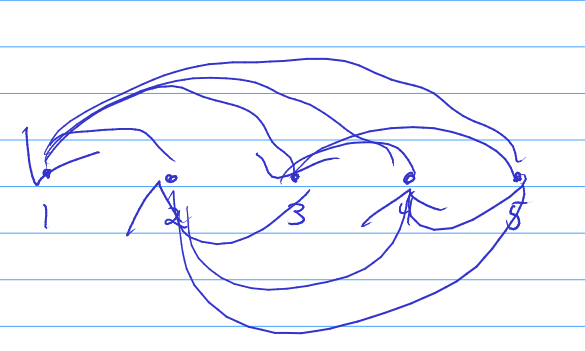
\includegraphics[width=0.7\textwidth]{images/11-01-01.png}
\end{figure}

\begin{exercise}{}{}
	{2. Let $A=\{1,2,3,4,5,6\}$. Write out the relation $R$ that expresses $\mid$ (divides) on $A$. Then illustrate it with a diagram.}
	\begin{alist}
		\item $R\subseteq A\times A = \set{(x, y): x\mid y}$.
	\end{alist}
\end{exercise}
\begin{figure}
	\centering
	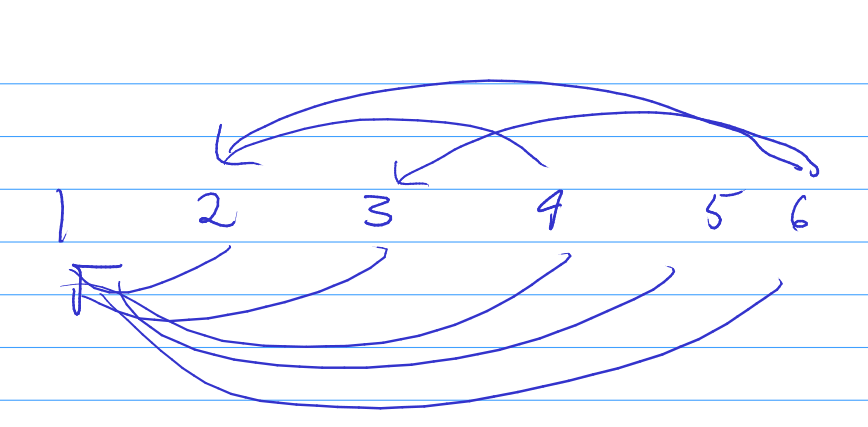
\includegraphics[width=0.7\textwidth]{images/11-01-02.png}
\end{figure}

\begin{exercise}{}{}
	{3. Let $A=\set{0,1,2,3,4,5}$. Write out the relation $R$ that expresses $\geq$ on $A$. Then illustrate it with a diagram.}
	\begin{alist}
		\item $R\subseteq A\times A = \set{(x, y): x-y \in \mathbb{N}}$.
		\item This relation defines a category. Take the diagram from the first problem and add identity arrows.
	\end{alist}
\end{exercise}

\begin{exercise}{}{}
	{4. Here is a diagram for a relation R on a set A. Write the sets A and R.}
	\begin{alist}
		\item $A = \set{0, 1, 2, 3, 4, 5, 6}$
		\item $R\subseteq A\times A =$
		\item
		\begin{tabular}{l}
			(0, 0) \\
			(0, 4) \\
			(1, 1) \\
			(1, 3) \\
			(1, 5) \\
			(2, 2) \\
			(2, 4) \\
			(3, 1) \\
			(3, 3) \\
			(4, 0) \\
			(4, 2) \\
			(4, 4) \\
			(5, 1) \\
			(5, 5)
		\end{tabular}
	\end{alist}
\end{exercise}
\begin{figure}
	\centering
	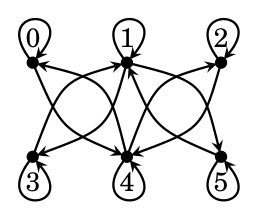
\includegraphics[width=0.4\textwidth]{images/11-01-04.png}
\end{figure}

\begin{exercise}{}{}
	{5. Here is a diagram for a relation $R$ on a set $A$. Write the
		sets $A$ and $R$.}
	\begin{alist}
		\item $A = \set{0, 1, 2, 3, 4, 5}$
		\item $R\subseteq A\times A =$
		\item
		\begin{tabular}{l}
			(1, 2) \\
			(2, 5) \\
			(3, 3) \\
			(4, 2) \\
			(4, 3) \\
			(5, 0)
		\end{tabular}
	\end{alist}
\end{exercise}
\begin{figure}
	\centering
	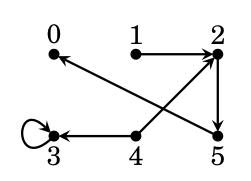
\includegraphics[width=0.4\textwidth]{images/11-01-05.png}
\end{figure}

\begin{exercise}{}{}
	{6. Congruence modulo 5 is a relation on the set $A=\mathbb{Z}$. In this relation $x R y$ means $x \equiv y(\bmod 5)$. Write out the set $R$ in set-builder notation.}
	\begin{alist}
		\item $R\subseteq A\times A = \set{(x, y) \in R: 5\mid x-y}$
	\end{alist}
\end{exercise}

\begin{exercise}{}{}
	{7. Write the relation $<$ on the set $A=\mathbb{Z}$ as a subset $R$ of $\mathbb{Z} \times \mathbb{Z}$. This is an infinite set, so you will have to use set-builder notation.}
	\begin{alist}
		\item $R\subseteq A\times A = \set{(x, y) \in R: y-x \in \mathbb{N}_{>0}}$
	\end{alist}
\end{exercise}

\begin{exercise}{}{}
	{8. Let $A=\{1,2,3,4,5,6\}$. Observe that $\varnothing \subseteq A \times A$, so $R=\varnothing$ is a relation on $A$. Draw a diagram for this relation.}
	\begin{alist}
		\item A diagram for a relation would have as points all elements of the set $R$.
		Because $R$ has no elements, the diagram is the empty diagram.
	\end{alist}
\end{exercise}

\begin{exercise}{}{}
	{9. Let $A = \set{1,2,3,4,5,6}$. How many different relations are there on the set A?}
	\begin{alist}
		\item This can be solved with the multiplication principle. There are 6 choices
		for two spots, therefore there are $6^2$ different pairs $A\times A$.
		\item A relation is any powerset of $A\times A$, therefore the problem is the
		equivalent of determining the cardinality of the powerset of $A\times A$,
		which is $2^{36}$.
	\end{alist}
\end{exercise}

\begin{exercise}{}{}
	{10. Consider the subset $R=(\mathbb{R} \times \mathbb{R})-\{(x, x): x \in
			\mathbb{R}\} \subseteq \mathbb{R} \times \mathbb{R}$. What familiar relation
		on $\mathbb{R}$ is this? Explain.}
	\begin{alist}
		\item This is the $\neq$ relation. We start with the full relation $\mathbb{R}
			\times \mathbb{R}$, and then substract all elements where the two elements
		are equal.  The universe minus the set where elements are equal leaves the
		unequal elements, therefore the $\neq$ relation.
	\end{alist}
\end{exercise}

\begin{exercise}{}{}
	{11. Given a finite set $A$, how many different relations are there on $A$ ?}
	\begin{alist}
		\item Let us suppose we are only considering binary relations. Then the total
		number of relations is $2^{|A|^2}$.
	\end{alist}
\end{exercise}

\begin{exercise}{}{}
	12-14. In the following exercises, subsets $R$ of $\mathbb{R}^2=\mathbb{R}
		\times \mathbb{R}$ or $\mathbb{Z}^2=\mathbb{Z} \times \mathbb{Z}$ are
	indicated by gray shading. In each case, $R$ is a familiar relation on
	$\mathbb{R}$ or $\mathbb{Z}$. State it.
	\begin{alist}
		\item 12. $R\subseteq \mathbb{R}\times\mathbb{R}\mid {x>y}$
		\item 13. $R\subseteq \mathbb{R}\times\mathbb{R}\mid {x\neq y}$
		\item 14. $R\subseteq \mathbb{R}\times\mathbb{R}\mid {x<y, x,y\in\mathbb{Z}}$
		\item 15. $R\subseteq \mathbb{R}\times\mathbb{R}\mid {x=y, x,y\in\mathbb{Z},
				x\mid 3}$
	\end{alist}
\end{exercise}
\begin{figure}
	\centering
	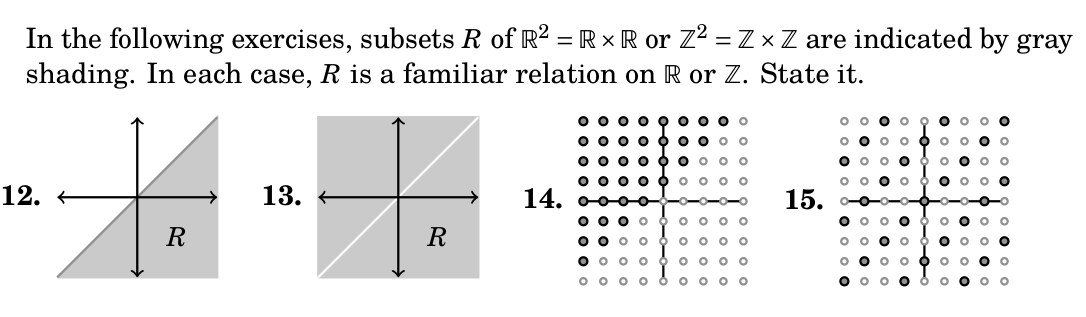
\includegraphics[width=0.9\textwidth]{images/11-01-12.png}
\end{figure}

\documentclass{hippoidC}

\memoto{Idris}
\memosubject{Book of Proof}
\memodate{2024.03.21}
\status{\S 11.2 Properties on Relations}

\begin{document}
\toc
\thispagestyle{styleTOC}
\pagebreak
\pagestyle{styleE}

\begin{prooflist}{1. Consider the relation $R=\set{(a, a),(b, b),(c, c),(d, d),(a,
				b),(b, a)}$ on set $A=\{a, b, c, d\}$. Is $R$ reflexive? Symmetric?
		Transitive? If a property does not hold, say why.}
	\item $R$ is reflective because $(x, x) \in R, \forall x \in A$.
	\item $R$ is symmetric because $(x, y) \in R \implies (y, x) \in R, \forall x,y \in A$.
	\item $R$ is transitive because $\forall (x, y), (y,z) \in R
		\implies (x, z) \in R, \forall x,y,z \in A$.
\end{prooflist}

\begin{prooflist}{2. Consider the relation $R=\set{(a, b),(a, c),(c, c),(b, b),(c,
				b),(b, c)}$ on the set $A=\set{a, b, c}$. Is $R$ reflexive? Symmetric?
		Transitive? If a property does not hold, say why.}
	\item $R$ is not reflective because $(a, a) \not\in R$.
	\item $R$ is not symmetric because $(a, b) \in R \not\implies (b, a) \in R$.
	\item $R$ is not transitive because $(b, c) \land (c, c) \in R \not \implies (b,
		c) \in R$.
\end{prooflist}

\begin{prooflist}{3. Consider the relation $R=\set{(a, b),(a, c),(c, b),(b, c)}$
		on the set $A=\set{a, b, c}$. Is $R$ reflexive? Symmetric? Transitive? If a
		property does not hold, say why.}
	\item $R$ is not reflective because $(a, a) \not\in R$.
	\item $R$ is not symmetric because $(a, b) \in R \not\implies (b, a) \in R$.
	\item $R$ is not transitive because $(c, b) \land (b, c) \in R \not \implies (c, c) \in R$.
\end{prooflist}

\begin{prooflist}{4. Let $A=\set{a, b, c, d}$. Suppose $R$ is the relation}
	\item
	\begin{align*}
		R= & (a, a),(b, b),(c, c),(d, d),(a, b),(b, a),(a, c),(c, a), \\
		   & (a, d),(d, a),(b, c),(c, b),(b, d),(d, b),(c, d),(d, c)
	\end{align*}
	\item $R$ is reflective because $(x, x) \in R, \forall x \in A$.
	\item $R$ is symmetric because $(x, y) \in R \implies (y, x) \in R, \forall x, y\in A$.
	\item $R$ is transitive because $|R|=16$, implying that all possible
	pairs of a $A$ are in $R$, including all the ones to satisfy the transitive
	property.
\end{prooflist}

\begin{prooflist}{5. Consider the relation $R=\{(0,0),(\sqrt{2}, 0),(0, \sqrt{2}),(\sqrt{2}, \sqrt{2})\}$ on $\mathbb{R}$. Is $R$ reflexive? Symmetric? Transitive? If a property does not hold, say why.}
	\item Let $A=\set{\sqrt{2}, 0}$.
	\item $R$ is reflective because $(x, x) \in R, \forall x \in A$.
	\item $R$ is symmetric because $(x, y) \in R \implies (y, x) \in R, \forall x, y\in A$.
	\item $R$ is transitive because $|R|=4, |A|=2, R=A\times A$, implying that all possible
	pairs of a $A$ are in $R$, including all the ones to satisfy the transitive
	property.
\end{prooflist}

\begin{prooflist}{6. Consider the relation $R=\{(x, x): x \in \mathbb{Z}\}$ on
		$\mathbb{Z}$. Is this $R$ reflexive? Symmetric? Transitive? If a property
		does not hold, say why. What familiar relation is this?}
	\item $R$ defines an equality relationship.  The equality relationship is
	reflexive, symmetric, and transitive, therefore R is all of those things.
\end{prooflist}

\begin{prooflist}{7. There are 16 possible different relations $R$ on the set $A=\{a, b\}$. Describe all of them. (A picture for each one will suffice, but don't forget to label the nodes.) Which ones are reflexive? Symmetric? Transitive?}
	\item Because $|A|=2$, there are 4 different pairs in $AxA$. The number of
	relatinoships is the powerset of $AxA$, and its cardinality is $2^4=16$.
	\item I'm not going to draw all of them.
\end{prooflist}

\begin{prooflist}{8. Define a relation $R$ on $\mathbb{Z}$ as $x R y$ if $|x-y|<1$. Is $R$ reflexive? Symmetric? Transitive? If a property does not hold, say why. What familiar relation is this?}
	\item The only way for two integers to be less
	than one apart, is for the the integers to be the same. Therefore $R$
	defines and equality relationship which is refesive, symmetric, and transitive.
\end{prooflist}

\begin{prooflist}{9. Define a relation on $\mathbb{Z}$ by declaring $x R y$ if and only if $x$ and $y$ have the same parity. Is $R$ reflexive? Symmetric? Transitive? If a property does not hold, say why. What familiar relation is this?}
	\item This relation is equivalent to a partition of $\mathbb{Z}$ into the evens
	and the odds.  Each partition also defines an equivalence class, and an
	equivalence class is by definition reflexive, symmetric, and transitive.
\end{prooflist}

\begin{prooflist}{10. Suppose $A \neq \varnothing$. Since $\varnothing \subseteq A \times A$, the set $R=\varnothing$ is a relation on $A$. Is $R$ reflexive? Symmetric? Transitive? If a property does not hold, say why.}
	\item The relation $R$ has cardinality 0. Therefore all of the implications
	necesarray to prove a relation is reflexive, symmetric, and transitive are
	all trivially true. Therefore $R$ is reflexive, symmetric, and transitive.
\end{prooflist}

\begin{prooflist}{11. Let $A=\{a, b, c, d\}$ and $R=\{(a, a),(b, b),(c, c),(d, d)\}$. Is $R$ reflexive? Symmetric? Transitive? If a property does not hold, say why.}
	\item $R$ defines an equality relationship which is reflexive, symmetric, and transitive.
\end{prooflist}

\begin{prooflist}{12. Prove that the relation $\mid$ (divides) on the set $\mathbb{Z}$ is reflexive and transitive. (Use Example 11.8 as a guide if you are unsure of how to proceed.)}
	\item Let $R$ be the relation $\mid$ (divides).
	\item $x \mid x \implies x \mid x$, therefore R is reflexive.
	\item Let us prove that $x \mid y \land y \mid z \implies x \mid z: x,y,z \in\mathbb{Z}$.
	\item Suppose $x\mid y$ and $y\mid z$. Therefore there exists some integers a
	and b such that $xa=y$ and $yb=z$. Thus $x(ab)=z$, which shows that $x\mid
		z$. Thusly we have shown that $R$ is transitive.
\end{prooflist}

\begin{prooflist}{13. Consider the relation $R=\{(x, y) \in \mathbb{R} \times \mathbb{R}: x-y \in \mathbb{Z}\}$ on $\mathbb{R}$. Prove that this relation is reflexive, symmetric and transitive.}
	\item Suppose $x - x \in \mathbb{Z}$.  By definition $x-x=0 \in \mathbb{Z}$,
	therefore $R$ is reflexive.
	\item Suppose $x - y \in \mathbb{Z}$. Therefore $x-y + y-x = 0$. Thus
	$y-x\in\mathbb{Z}$. Thus $R$ is symmetric.
	\item Suppose $x - y \in \mathbb{Z} \land y - z\in\mathbb{Z}$. Therefore $x-z =
		(x-y) + (y-z)$. Since both $x-y$ and $y-z$ are integers, the difference of those
	two quantities is also an integer, and therefore $x-z\in\mathbb{Z}$, and
	thus $R$ is transitive.
\end{prooflist}

\begin{prooflist}{14. Suppose $R$ is a symmetric and transitive relation on a
		set $A$, and there is an element $a \in A$ for which $Rax$ for every $x
			\in A$. Prove that $R$ is reflexive.}
	\item Because $R$ is symmetric, then $Rxy \implies Ryx$.
	\item Because $R$ is transitive, then $R x y \land Ryz \implies Rxz$.
	\item Suppose some relation $Rxa\implies Rax$ because of symmetry.
	\item $Rxa \land Rax \implies Rxx$ because of transitivity. Therefore we have
	shown $R$ is also reflexive.
\end{prooflist}

\begin{prooflist}{15. Prove or disprove: If a relation is symmetric and transitive, then it is also reflexive.}
	\item $Rxy \implies Ryx$, due to symmetry.
	\item $Rxy \land Ryx \implies Rxx$, due to transitivity.
	\item Therefore a relation being symmetric and transitive implies the relation
	is also reflexive.
\end{prooflist}

\begin{prooflist}{16. Define a relation $R$ on $\mathbb{Z}$ by declaring that $x R y$ if and only if $x^2 \equiv y^2(\bmod 4)$. Prove that $R$ is reflexive, symmetric and transitive.}
	\item Let $(x, y) \in R\subseteq \mathbb{Z}\times\mathbb{Z}; x^2\equiv y^2\bmod 4$.
	\item Suppose $(x, y)$ in $R$. Therefore $4 | x^2 - y^2$. If $x=y$, then $4\mid
		0$, which is always true, therefore $R$ is reflexive.
	\item Suppose $(x, y)$ in $R$. Therefore $4 | x^2 - y^2$. Hence, there exists
	some integer $a$ such that $4a = x^2-y^2$. Multiplying both sides by $-1$
	and we get $-4a = y^2-x^2$.  If a number is divisible by $n$, then it is also
	divisble by $-n$.
	\item Suppose $(x, y)\land (y, z)$ in $R$. Therefore $4 \mid x^2 - y^2 \land
		4\mid y^2-z^2$. Hence, there exists integers $a$ and $b$ such that $4a =
		x^2-y^2$ and $4b=y^2-z^2$. Adding the two equations together yields
	$4(a+b) = x^2 -z^2$, which shows $4\mid x^2 - z^2$, and thus $R$ is
	transitive.
\end{prooflist}

\begin{prooflist}{17. Modifying Exercise 8 (above) slightly, define a relation
		$\sim$ on $\mathbb{Z}$ as $x \sim y$ if and only if $|x-y| \leq 1$. Say
		whether $\sim$ is reflexive. Is it symmetric? Transitive?}
	\item For any integer $x$, $|x-x| \leq 1$, therefore $R$ is reflexive.
	\item This relation holds for any integers which are either equal are
	consecutive. Assume some integer $x$ and its consecutive integer $x+1$.
	Therefore $|x-x-1|=1\leq 1 \implies |x+1-x|=1 \leq 1$.
	For the case of $Rxx$, $|x-x|=0 < 1 \implies 0 < 1$, therefore $R$ is symmetric.
	\item This relation is not transitive. For example $2R3 \land 3R4 \not\implies
		2R4$.
\end{prooflist}

\begin{prooflist}{18. The table on page 205 shows that relations on Z may obey
		various combinations of the reflexive, symmetric and transitive
		properties. In all, there are 23 = 8 possible combinations, and the
		table shows 5 of them. (There is some redundancy, as $\neq$ and $\mid$
		have the same type.) Complete the table by finding examples of relations
		on Z for the three missing combinations.}
	\item
	\begin{tabular}{|c|c|c|c|}
		\hline
		\textbf{Reflexive}  & \textbf{Symmetric} & \textbf{Transitive} & \textbf{Example}              \\
		\hline $\checkmark$ & $\checkmark$       & $\checkmark$        & $=$                           \\
		\hline $\checkmark$ & $\checkmark$       &                     & $x-y\leq 1; x,y\in\mathbb{Z}$ \\
		\hline $\checkmark$ &                    & $\checkmark$        & $\leq$                        \\
		\hline              & $\checkmark$       & $\checkmark$        & none                          \\
		\hline $\checkmark$ &                    &                     & none                          \\
		\hline              & $\checkmark$       &                     & $\neq$                        \\
		\hline              &                    & $\checkmark$        & $\set{(1,2), (2, 3), (1, 3)}$ \\
		\hline              &                    &                     & $\set{1,3}$                   \\
		\hline
	\end{tabular}
\end{prooflist}


\end{document}

\documentclass{hippoidC}

\memoto{Idris}
\memosubject{Book of Proof}
\memodate{2024.03.21}
\status{\S 11.3 Equivalence Relations}

\begin{document}
\toc
\thispagestyle{styleTOC}
\pagebreak
\pagestyle{styleE}

\begin{prooflist}{1. Let $A=\{1,2,3,4,5,6\}$, and consider the following
    equivalence relation on $A$ :
    \[
R=\set{(1,1),(2,2),(3,3),(4,4),(5,5),(6,6),(2,3),(3,2),(4,5),(5,4),(4,6),(6,4),(5,6),(6,5)}
\]
List the equivalence classes of $R$.
}
\item $[1]=\set{(1, 1)}$
\item $[2]=\set{(2, 2), (2, 3), (3, 2), (3, 3)}$
\item $[4]=\set{(4, 4), (4, 5), (5, 4), (4, 6), (6, 4), (5,5), (5, 6), (6, 5) }$
\end{prooflist}

\begin{prooflist}{2. Let $A=\{a, b, c, d, e\}$. Suppose $R$ is an equivalence
    relation on $A$. Suppose $R$ has two equivalence classes. Also $a R d, b R
c$ and $e R d$. Write out $R$ as a set.}
\item $[a] = \set{(a, a), (d, d), (e, e), (a, d), (d, a), (d, e), (e, d), (e,
    a), (a, e)}$.
\item $[b] = \set{(b, b), (c, c), (b, c), (c, b)}$.
\end{prooflist}

\begin{prooflist}{3. Let $A=\{a, b, c, d, e\}$. Suppose $R$ is an equivalence
relation on $A$. Suppose $R$ has three equivalence classes. Also $a R d$ and $b
R c$. Write out $R$ as a set.}
\item $[a] = \set{(a, a), (d, d), (a, d), (d, a)}$.
\item $[b] = \set{(b, b), (c, c), (b, c), (c, b)}$.
\item $[e] = \set{(e, e)}$.
\end{prooflist}

\begin{prooflist}{4. Let $A=\{a, b, c, d, e\}$. Suppose $R$ is an equivalence
relation on $A$. Suppose also that $a R d$ and $b R c, e R a$ and $c R e$. How
many equivalence classes does $R$ have?}
\item $a$ is related to $d$ and $e$, which is related to $c$, which is related
    to $b$. Therefore this one equivalence class traverses the entire set, so
    there is just one equivalence class.
\end{prooflist}

\begin{prooflist}{5. There are two different equivalence relations on the set
$A=\{a, b\}$. Describe them. Diagrams will suffice.}
\item One equivalence relation is $\set{(a, a), (a, b), (b, a), (b, b)}$.
\item One equivalence relation is $\set{(a, a), (b, b)}$.
\end{prooflist}

\begin{prooflist}{6. There are five different equivalence relations on the set
$A=\{a, b, c\}$. Describe them all. Diagrams will suffice.}
\item One equivalence relation admits 1 equivalence class which has $a=b=c$.
\item One equivalence relation admits 2 equivalence classes which has $a=b\neq c$.
\item One equivalence relation admits 2 equivalence classes which has $a=c\neq b$.
\item One equivalence relation admits 3 equivalence classes which has $b=c\neq a$.
\item One equivalence relation admits 3 equivalence classes which has $a\neq b\neq c$.
\end{prooflist}

\begin{prooflist}{7. Define a relation $R$ on $\mathbb{Z}$ as $x R y$ if and
only if $3 x-5 y$ is even. Prove $R$ is an equivalence relation. Describe its
equivalence classes.}
\item $R\subseteq \mathbb{Z}\times\mathbb{Z}\mid 3x-5y=2c, c\in\mathbb{N}$.
\item For any $x, y$, $3x+5y=3x+5y$, therefore $R$ is reflexive.
\item For any $x, y$, $3x+5y=2c$, for some integer $c$. Because $3x+5y$ is even,
    $x$ and $y$ must have the same parity.  Therefore $3y+5x$ will also be even,
    thus we have shown $R$ is symmetric.
\item For any $x, y, z$, $3x+5y=2c \land 3y+5z=2d$, for some integers $c, d$.
    Because $3x+5y$ is even, $x$ and $y$ must have the same parity.
    Because $3y+5z$ is even, $y$ and $z$ must have the same parity. Therefore,
    $x$ and $z$ have the same parity and we have shown that $R$ is transitive.
\item Because $R$ is reflexive, symmetric, and transitive, it is an equivalence
    relation.
\item Now that we have proven $R$ is an equivalence relation, we can show its
    equivalence classes. The equivalence classes are defined by parity,
    therefore all evens form one class, and the odds another class.
\end{prooflist}

\begin{prooflist}{8. Define a relation $R$ on $\mathbb{Z}$ as $x R y$ if and
only if $x^2+y^2$ is even. Prove $R$ is an equivalence relation. Describe its
equivalence classes.}
\item For any $x, y$, $x^2+y^2=2c=x^2+y^2$, for some integer $c$. Therefore $R$
    is reflexive.
\item For any $x, y$, $x^2+y^2=2c$. Suppose $x=2a$ and $y=2b+1$, then
    $x^2+y^2 = 4a^2 + 4b^2 + 4b + 1 = 2(a^2 + b^2 + 2b) + 1$, which is not even.
    Therefore x cannot be odd while y is even. Through a similar procedure, we
    can show that x cannot be even while y is odd. Therefore $x$ and $y$ cannot
    have a different parity for the relation to hold.
\item For any $x, y$, $x^2+y^2=2c$. Suppose $x=2a$ and $y=2b$, then
    $x^2+y^2 = 4a^2 + 4b^2 = 2(a^2 + b^2)$, which is even.
    Therefore x and y both being even numbers will let the relation hold.
\item For any $x, y$, $x^2+y^2=2c$. Suppose $x=2a+1$ and $y=2b+1$, then
    $x^2+y^2 = 4a^2 + 4a + 1 + 4b^2 + 4b + 1 = 2(a^2 + b^2 + 2b + 2a + 1)$, which is even.
    Therefore x and y both being odd numbers will let the relation hold.
\item If x and y have the same parity, then $x^2+y^2$ is even and also $y^2+x^2$
    will be even. Therefore $R$ is symmetric.
\item If x and y and z have the same parity, then $x^2+y^2$ is even $y^2+z^2$ is
    even, and $x^2+y^2-y^2 + z^2$, will be the difference between two even
    integers, which is also even. Therefore $R$ is transitive.
\item The set $\mathbb{Z}$ is partitioned into two classes over the relation
    $R$, namely the evens and odds.
\end{prooflist}

\begin{prooflist}{9. Define a relation $R$ on $\mathbb{Z}$ as $x R y$ if and
only if $4 \mid(x+3 y)$. Prove $R$ is an equivalence relation. Describe its
equivalence classes.}
\item
    \begin{align*}
        4 &\mid(x+3 y)\\
        4a &=x+3 y
    \end{align*}
\item For any $x,y\in\mathbb{Z}$, $4a=x+3y=x+3y$, for some integer $a$,
    therefore $R$ is reflexive.
\item For any $x,y\in\mathbb{Z}$, $4a=x+3y$, for some integer $a$.
    \begin{align*}
        4a&=x+3y\\
        4(4a)&=4x+12y\\
        4(4a)&=(y+3x) + (x+3y) + 8y\\
        4(4a)&=(y+3x) + 4a + 8y\\
        4(3a)-4(2y)&=y+3x\\
        4(3a-2y)&=y+3x\\
    \end{align*}
    Therefore $4\mid y+3x$, and $R$ is symmetric.
\item For any $x,y,z\in\mathbb{Z}$, $4a=x+3y \land 4b=y+3z$, for some integers $a, b$.
    \begin{align*}
        4a&=x+3y\\
        4b&=y+3z\\
        4(a+b)&=x+3y+y+3z\\
        4(a+b)&=x+4y+3z\\
        4(a+b-y)&=x+3z
    \end{align*}
\item Therefore $R$ is transitive.
\end{prooflist}

\begin{prooflist}{10. Suppose $R$ and $S$ are two equivalence relations on a set
    $A$. Prove that $R \cap S$ is also an equivalence relation. (For an example
of this, look at Figure 11.2. Observe that for the equivalence relations $R_2,
R_3$ and $R_4$, we have $R_2 \cap R_3=R_4$.)}
\item Suppose $(x, x) \in R\cap S$. Therefore $(x, x)$ is also in $R \cap S$ and
    we have shown the intersection is reflexive.
\item Suppose $(x, y) \in R\cap S$.  Because $R$ and $S$ are both equivalence
    relations, $(y, x$) is in both $R$ and $S$ and therefore it will also be in
    $R\cap S$, by the definition of intersection. Therefore $R\cap S$ is
    symmetric.
\item Suppose $(x, y), (y, z) \in R\cap S$.  Because $R$ and $S$ are both equivalence
    relations, $(x, z$) is in both $R$ and $S$ and therefore it will also be in
    $R\cap S$, by the definition of intersection. Therefore $R\cap S$ is
    transitive.
\item Because $R\cap S$ is reflexive, symmetric, and transitive, we have shown
    that $R\cap S$ is an equivalence relation.
\end{prooflist}

\begin{prooflist}{11. Prove or disprove: If $R$ is an equivalence relation on an
infinite set $A$, then $R$ has infinitely many equivalence classes.}
\item Suppose $A=\mathbb{Z}$, and $R$ is the equivalence relation defined by an
    integer's parity. Therefore there will be equivalence classes (even and
    odd).
\item Therefore, by example, we have shown an example of an infinite set with a
    finite number of equivalence classes, thus disproving the statement
    \quote{
    If $R$ is an equivalence relation on an
    infinite set $A$, then $R$ has infinitely many equivalence classes.
}
\end{prooflist}

\begin{prooflist}{12. Prove or disprove: If $R$ and $S$ are two equivalence
relations on a set $A$, then $R \cup S$ is also an equivalence relation on $A$.}
\item Suppose $(x, x) \in R\cup S$. Therefore $(x, x)$ is also in $R \cup S$ and
    we have shown the intersection is reflexive.
\item Suppose $(x, y) \in R\cup S$.  Because $R$ and $S$ are both equivalence
    relations, $(y, x$) is in both $R$ or $S$ and therefore it will also be in
    $R\cup S$, by the definition of union. Therefore $R\cup S$ is
    symmetric.
\item Suppose $(x, y)\in R \land (y, z) \in S$. Therefore $(x, z), (y, z)$ will
    be in $R\cup S$. For $R\cup S$ to be transitive, $(x, z)$ must be in either
    $R$ or $S$, but there is no justification to believe it is in either.
    Therefore we can not prove that $R\cup S$ is transitive.
\item Because $R\cup S$  we cannot prove that $R\cup S$ is transitive, it is not
    an equivalence relation.
\end{prooflist}

\begin{prooflist}{13. Suppose $R$ is an equivalence relation on a finite set
$A$, and every equivalence class has the same cardinality $m$. Express $|R|$
in terms of $m$ and $|A|$.}
\item
    \begin{align*}
    |R| = m \cdot |A|
\end{align*}
\end{prooflist}

\begin{prooflist}{14. Suppose $R$ is a reflexive and symmetric relation on a
    \mbox{finite set $A$.}}
\item Define a relation $S$ on $A$ by declaring $x S y$,
\item if and only if for some $n \in \mathbb{N}$ there are elements $x_1, x_2, \ldots, x_n \in A$
\item satisfying $x R x_1, x_1 R x_2, x_2 R x_3, x_3 R x_4, \ldots, x_{n-1} R x_n$, and $x_n R y$
\item Show that $S$ is an equivalence relation and $R \subseteq S$.
\item Prove that $S$ is the unique smallest equivalence relation on $A$ containing $R$.
    \begin{align*}
        A=&\set{1, 2, 9}\\
        R\subseteq A\times A=&\set{(1, 1), (2, 2), (9, 9), (2, 9), (9, 2)}\\
        4S\subseteq A\times A=&\set{}
    \end{align*}
\end{prooflist}

\begin{prooflist}{15. Suppose $R$ is an equivalence relation on a set $A$, with
four equivalence classes. How many different equivalence relations $S$ on $A$
are there for which $R \subseteq S$ ?}
\item $R$ can be partitioned into 4 different subsets, each one an equivalence
    class.
\item Let $T$ be the set with elements that are the equivalence classes of $R$.
\item Each element of $T$ is also an equivalence relation. The
    intersection of equivalence relations yields another equivalence
    relation.Therefore this question is the same as for the cardinality of the
    powerset of $T$.
\item Therefore there are $\mathscr{P}(T) = 2^4 = 16$.
\item But the answer in the book is 15...?
\end{prooflist}

\begin{prooflist}{16. Show that the relation $\doteq$ defined on page 213 is
transitive.} \item \end{prooflist}

\end{document}

\documentclass{article}
\makeindex

\usepackage{amsmath}
\usepackage{amssymb}
\usepackage{booktabs}
\usepackage{csvsimple-l3}
\usepackage{bussproofs}
\usepackage{dirtytalk}
\usepackage[dvipsnames]{xcolor}
\usepackage{enumitem}
\usepackage{epigraph}
\usepackage{forest}
\usepackage{formal-grammar}
\usepackage{graphicx}
\usepackage[citecolor=blue,colorlinks=true, linkcolor=blue, urlcolor=blue]{hyperref}
\usepackage{kantlipsum}
\usepackage{makeidx}
\usepackage[margin=0.8in]{geometry}
\usepackage{mathrsfs}
\usepackage[outputdir=../build]{minted}
\usepackage{multicol}
\usepackage[mode=tex]{standalone}
\usepackage[style=authortitle]{biblatex}
\usepackage[T1]{fontenc}
\usepackage[tableaux]{prooftrees}
\usepackage{tcolorbox}
\usepackage{tikz}
\usepackage{titlesec}
\usepackage{xcolor}

\usetikzlibrary{arrows}
\usetikzlibrary{arrows.meta}
\usetikzlibrary{automata}
\usetikzlibrary{calc}
\usetikzlibrary{fit}
\usetikzlibrary{petri}
\usetikzlibrary{positioning}

\tcbuselibrary{breakable}
\tcbuselibrary{listings}
\tcbuselibrary{minted}
\tcbuselibrary{skins}
\tcbuselibrary{theorems}

\newcounter{filePrg}

\addbibresource{biblio.bib}
\setlength{\parindent}{0pt}

\renewcommand{\emph}[1]{\textit{#1}}
\setlength{\parindent}{0pt}

\newcommand\setboxcounter[2]{\setcounter{tcb@cnt@#1}{#2}}
\newcommand\qed[0]{\blacksquare}
\setlength{\parindent}{10pt}
\newcommand{\set}[1]{\{#1\}}
\newcommand{\up}[1]{ \left\lceil#1\right\rceil }
\newcommand{\down}[1]{ \left\lfloor#1\right\rfloor}

\definecolor{CaribbeanBlue}{RGB}{0, 206, 209} % Define Caribbean Blue
\NewTcbTheorem[list inside=definition]{definition}
{Definition}{
	breakable,
	colback=CaribbeanBlue!05,
	colframe=CaribbeanBlue!35!black,
	fonttitle=\bfseries}{th}

\NewTcbTheorem[list inside=intuition]{intuition}{Intuition}{
	breakable,
	colback=blue!5,
	colframe=blue!35!black,
	fonttitle=\bfseries}{th}

\NewTcbTheorem{example}{Example}{
	breakable,
	colback=white,
	colframe=green!35!black,
	fonttitle=\bfseries}{th}

\NewTcbTheorem{verify}{Verify}{
	breakable,
	float,
	colback=red!5,
	colframe=red!35!black,
	fonttitle=\bfseries}{th}

\NewTcbTheorem[list inside=theorem]{theorem}{Theorem}{
	breakable,
	colback=gray!10,
	colframe=gray!35!black,
	fonttitle=\bfseries}{th}

% \NewTcbTheorem[
% list inside=exercise,
% number within=chapter,
% number within=section,
% ]

\NewTcbTheorem[
	list inside=exercise,
	number within=section,
]{exercise}{Exercise}{
	breakable,
	colback=white,
	colframe=black,
	fonttitle=\bfseries}{th}

\newcommand{\hask}[1]{\mintinline{haskell}{#1}}

\newenvironment{alist}
{\begin{enumerate}[label={*}, leftmargin=*, itemsep=0pt, parsep=0pt]}
		{\end{enumerate}}

\newenvironment{blist}
{\begin{enumerate}[label={}, leftmargin=*, itemsep=0pt, parsep=0pt]}
		{\end{enumerate}}

\renewcommand{\thesection}{\arabic{section}}
\tcbset{enhanced jigsaw}

\newtcbinputlisting{\codeFromFile}[2]{
	listing file={#1},
	listing engine=minted,
	minted style=colorful,
	minted language=haskell,
	minted options={breaklines,linenos,numbersep=3mm},
	colback=blue!5!white,colframe=blue!75!black,listing only,
	left=5mm,enhanced,
	title={#2},
	overlay={\begin{tcbclipinterior}\fill[red!20!blue!20!white] (frame.south west)
				rectangle ([xshift=5mm]frame.north west);\end{tcbclipinterior}}
}

\newtcblisting{haskell}[1]
{
	listing engine=minted,
	minted style=colorful,
	minted language=haskell,
	minted options={breaklines,linenos,numbersep=3mm},
	colback=blue!5!white,colframe=blue!75!black,listing only,
	left=5mm,enhanced,
	title={#1},
	overlay={\begin{tcbclipinterior}\fill[red!20!blue!20!white] (frame.south west)
				rectangle ([xshift=5mm]frame.north west);\end{tcbclipinterior}}
}


\begin{document}
\section{Equivalence Classes and Partitions}
\begin{exercise}{}{}
	{1. List all the partitions of the set $A=\{a, b\}$. Compare your answer to
		the answer to Exercise 5 of Section 11.3.}
	\begin{alist}
		\item
		\begin{align*}
			\set{\set{a}, \set{b}} \\
			\set{\set{a, b}}
		\end{align*}
	\end{alist}
\end{exercise}{}{}

\begin{exercise}{}{}{2. List all the partitions of the set $A=\{a, b, c\}$. Compare
		your answer to the answer to Exercise 6 of Section 11.3.}
	\begin{alist}
		\item
		\begin{align*}
			\set{\set{a}, \set{b}, \set{c}} \\
			\set{\set{a, b}, \set{c}}       \\
			\set{\set{a, c}, \set{b}}       \\
			\set{\set{b, c}, \set{a}}       \\
			\set{\set{a, b, c}}
		\end{align*}
		\item
	\end{alist}
\end{exercise}{}{}

\begin{exercise}{}{}
	{3. Describe the partition of $\mathbb{Z}$ resulting from the equivalence
		relation $\equiv(\bmod 4)$.}
	\begin{alist}
		\item Let $R$ be the relation $\equiv\bmod 4$.
		\item For any integer $a$, the value of $a\bmod 4$ is in the set $\set{0, 1, 2, 3}$.
		\item Therefore each element in $\set{0, 1, 2, 3}$ defines an equivalence class
		on $\mathbb{Z}$ from the equivalence relation $\equiv(\bmod 4)$.
		\item Thus the 4 equivalence classes are
		\begin{align*}
			\set{-15, -11, -7, -3, 1 \dots x\bmod4=3} \\
			\set{-14, -10, -6, -2, 2 \dots x\bmod4=2} \\
			\set{-13, -9, -4, -1, 3 \dots x\bmod4=1}  \\
			\set{-12, -8, -4, 0, 4 \dots x\bmod4=0}   \\
		\end{align*}
	\end{alist}
\end{exercise}{}{}

\begin{exercise}{}{}{4. Suppose $P$ is a partition of a set $A$. Define a
		relation $R$ on $A$ by declaring $x R y$ if and only if $x, y \in X$ for
		some $X \in P$. Prove $R$ is an equivalence relation on $A$. Then prove that $P$
		is the set of equivalence classes of $R$.}
	\begin{alist}
		\item Let $P$ be a partition of set $A$.
		\item Define relation $R$ on $A$ as follows: $x R y$ if and only if $x$
		and $y$ belong to the same set $X \in P$.
		\item To prove $R$ is an equivalence relation:
		\begin{itemize}
			\item Reflexivity: For any $x \in A$, since $x$ belongs to some set
			      $X \in P$, $x R x$ by definition. Hence, $R$ is reflexive.
			\item Symmetry: If $x R y$, then $x$ and $y$ belong to the same set
			      $X \in P$. But this also means $y$ and $x$ belong to the same
			      set $X$, so $y R x$. Thus, $R$ is symmetric.
			\item Transitivity: If $x R y$ and $y R z$, then both $x$ and $y$,
			      and $y$ and $z$, belong to the same sets $X$ and $Y$ in $P$
			      respectively. Since $P$ is a partition, $X$ and $Y$ are either
			      identical or disjoint. If they are identical, then $x R z$
			      trivially. If they are disjoint, then $x$ and $z$ cannot belong
			      to the same set in $P$, so $x R z$ holds vacuously. In either
			      case, $R$ is transitive.
		\end{itemize}
		\item Now, to prove that $P$ is the set of equivalence classes of $R$:
		\begin{itemize}
			\item Each set $X \in P$ is an equivalence class of $R$: By
			      definition, elements in the same set $X$ under $P$ are related
			      by $R$. So, $P$ consists of equivalence classes of $R$.
			\item Every equivalence class of $R$ is a set in $P$: Since $P$ is a
			      partition, each element of $A$ belongs to exactly one set $X \in
				      P$. Thus, each equivalence class of $R$ corresponds to a set in
			      $P$.
		\end{itemize}
	\end{alist}
\end{exercise}{}{}

\begin{exercise}{}{}
	{5. Consider the partition $P=\{\{\ldots,-4,-2,0,2,4,
			\ldots\},\{\ldots,-5,-3,-1,1,3,5, \ldots\}\}$ of $\mathbb{Z}$. Let $R$ be
		the equivalence relation whose equivalence classes are the two elements of $P$.
		What familiar equivalence relation is $R$ ?}
	\begin{alist}
		\item $xRy$ is true when $x$ and $y$ have the same parity.
	\end{alist}
\end{exercise}{}{}

\begin{exercise}{}{}
	{6. Consider the partition
		$P=\{\{0\},\{-1,1\},\{-2,2\},\{-3,3\},\{-4,4\}, \ldots\}$ of $\mathbb{Z}$.
		Describe the equivalence relation whose equivalence classes are the elements of
		$P$.}
	\begin{alist}
		\item $xRy$ is defined by $|x|=|y|$.
	\end{alist}
\end{exercise}{}{}

\end{document}

\documentclass{hippoidC}

\memoto{Idris}
\memosubject{Book of Proof}
\memodate{2024.03.21}
\status{\S 11.5 Integer Modulo n}

\begin{document}
\toc
\thispagestyle{styleTOC}
\pagebreak
\pagestyle{styleE}

\begin{prooflist}{1. Write the addition and multiplication tables for $\mathbb{Z}_2$.}
	\item
	\[
		\begin{array}{c|cc}
			\times & 0 & 1 \\
			\hline
			0      & 0 & 0 \\
			1      & 0 & 1 \\
		\end{array}
	\]
	\item
	\[
		\begin{array}{c|cc}
			+ & 0 & 1 \\
			\hline
			0 & 0 & 1 \\
			1 & 1 & 0 \\
		\end{array}
	\]
\end{prooflist}

\begin{prooflist}{2. Write the addition and multiplication tables for $\mathbb{Z}_3$.}
	\item \[
		\begin{array}{c|ccc}
			\times & 0 & 1 & 2 \\
			\hline
			0      & 0 & 0 & 0 \\
			1      & 0 & 1 & 2 \\
			2      & 0 & 2 & 1 \\
		\end{array}
	\]
	\item \[
		\begin{array}{c|ccc}
			+ & 0 & 1 & 2 \\
			\hline
			0 & 0 & 1 & 2 \\
			1 & 1 & 2 & 0 \\
			2 & 2 & 0 & 1 \\
		\end{array}
	\]
\end{prooflist}

\begin{prooflist}{3. Write the addition and multiplication tables for $\mathbb{Z}_4$.}
	\item \[
		\begin{array}{c|cccc}
			\times & 0 & 1 & 2 & 3 \\
			\hline
			0      & 0 & 0 & 0 & 0 \\
			1      & 0 & 1 & 2 & 3 \\
			2      & 0 & 2 & 0 & 2 \\
			3      & 0 & 3 & 2 & 1 \\
		\end{array} \]
	\item \[
		\begin{array}{c|cccc}
			+ & 0 & 1 & 2 & 3 \\
			\hline
			0 & 0 & 1 & 2 & 3 \\
			1 & 1 & 2 & 3 & 0 \\
			2 & 2 & 3 & 0 & 1 \\
			3 & 3 & 0 & 1 & 2 \\
		\end{array} \]

\end{prooflist}

\begin{prooflist}{4. Write the addition and multiplication tables for $\mathbb{Z}_6$.}
	\item \[
		\begin{array}{c|cccccc}
			\times & 0 & 1 & 2 & 3 & 4 & 5 \\
			\hline
			0      & 0 & 0 & 0 & 0 & 0 & 0 \\
			1      & 0 & 1 & 2 & 3 & 4 & 5 \\
			2      & 0 & 2 & 4 & 0 & 2 & 4 \\
			3      & 0 & 3 & 0 & 3 & 0 & 3 \\
			4      & 0 & 4 & 2 & 0 & 4 & 2 \\
			5      & 0 & 5 & 4 & 3 & 2 & 1 \\
		\end{array}
	\]
	\item \[
		\begin{array}{c|cccccc}
			+ & 0 & 1 & 2 & 3 & 4 & 5 \\
			\hline
			0 & 0 & 1 & 2 & 3 & 4 & 5 \\
			1 & 1 & 2 & 3 & 4 & 5 & 0 \\
			2 & 2 & 3 & 4 & 5 & 0 & 1 \\
			3 & 3 & 4 & 5 & 0 & 1 & 2 \\
			4 & 4 & 5 & 0 & 1 & 2 & 3 \\
			5 & 5 & 0 & 1 & 2 & 3 & 4 \\
		\end{array}
	\]
\end{prooflist}

\begin{prooflist}{5. Suppose $[a],[b] \in \mathbb{Z}_5$ and $[a] \cdot[b]=[0]$.
		Is it necessarily true that either $[a]=[0]$ or $[b]=[0]$ ?}
	\item Assume: $[a]\cdot[b]=[0]$ for some $[a],[b]\in\mathbb{Z}_5$.
	\item Translate: This means $[a\cdot b]\equiv[0]$, so $a\cdot b\equiv 0\bmod 5$
	\item Property of Modulo 5: This implies that 5 divides the product $a\cdot b$.
	\item Prime Divisibility: Since 5 is a prime number, it must divide either a or b.
	\item Back to Equivalence Classes: Therefore, $a \equiv 0 \pmod 5$ (meaning
	$[a]=[0]$) or $b \equiv 0 \pmod 5$ (meaning $[b]=[0]$).
	\item \[
		\begin{array}{c|ccccc}
			\times & 0 & 1 & 2 & 3 & 4 \\
			\hline
			0      & 0 & 0 & 0 & 0 & 0 \\
			1      & 0 & 1 & 2 & 3 & 4 \\
			2      & 0 & 2 & 4 & 1 & 3 \\
			3      & 0 & 3 & 1 & 4 & 2 \\
			4      & 0 & 4 & 3 & 2 & 1 \\
		\end{array}
	\]
\end{prooflist}

\begin{prooflist}{6. Suppose $[a],[b] \in \mathbb{Z}_6$ and $[a] \cdot[b]=[0]$. Is it necessarily true that either $[a]=[0]$ or $[b]=[0]$ ? What if $[a],[b] \in \mathbb{Z}_7$ ?}
	\item Assume: $[a]\cdot[b]=[0]$ for some $[a],[b]\in\mathbb{Z}_6$.
	\item Translate: This means $[a\cdot b]\equiv[0]$, so $a\cdot b\equiv 0\bmod 6$
	\item Property of Modulo 6: This implies that 6 divides the product $a\cdot b$.
	\item Prime Divisibility: Since the prime factors of 6 are 2 and 3, 2 must
	factor a or b and 3 must factor a or b. Assume $3\mid a \land 2\mid b$. Let
	$a=3$ and $b=2$, and then $a\cdot b \equiv 0 \mod 6$.
	\item Back to Equivalence Classes: Therefore, it's not necessarily true that
	either $[a] = [0] \lor [b] = [0]$ when $[a]\cdot[b]=[0]$ for $\mathbb{Z}_6$.
	\item Assume: $[a]\cdot[b]=[0]$ for some $[a],[b]\in\mathbb{Z}_7$.
	\item Translate: This means $[a\cdot b]\equiv[0]$, so $a\cdot b\equiv 0\bmod 6$
	\item Property of Modulo 7: This implies that 7 divides the product $a\cdot b$.
	\item Prime Divisibility: Since 7 is a prime number, it must divide either a or b.
	\item Back to Equivalence Classes: Therefore, $a \equiv 0 \pmod 7$ (meaning
	$[a]=[0]$) or $b \equiv 0 \pmod 7$ (meaning $[b]=[0]$).
\end{prooflist}

\begin{prooflist}{7. Do the following calculations in $\mathbb{Z}_9$, in each case expressing your answer as $[a]$ with $0 \leq a \leq 8$.}
	\item
	      (a) $[8]+[8] = [7]$
	\item
	      (b) $[24]+[11] = [8]$
	\item
	      (c) $[21] \cdot[15] = [0]$
	\item
	      (d) $[8] \cdot [8] = [1]$
\end{prooflist}

\begin{prooflist}{8. Suppose $[a],[b] \in \mathbb{Z}_n$, and $[a]=\left[a^{\prime}\right]$ and $[b]=\left[b^{\prime}\right]$. Alice adds $[a]$ and $[b]$ as $[a]+[b]=$ $[a+b]$. Bob adds them as $\left[a^{\prime}\right]+\left[b^{\prime}\right]=\left[a^{\prime}+b^{\prime}\right]$. Show that their answers $[a+b]$ and $\left[a^{\prime}+b^{\prime}\right]$ are the same.}
	\item
\end{prooflist}

\end{document}


\chapter{Function}
\section{Functions}
\begin{exercise}{}{}
	Suppose $A=\{0,1,2,3,4\}, B=\{2,3,4,5\}$ and\\
	$f=\{(0,3),(1,3),(2,4),(3,2),(4,2)\}$. State the domain and range of $f$.
	Find $f(2)$ and $f(1)$.
	\tcblower
	\begin{alist}
		\item Domain is $A$.
		\item Rance is $\set{3, 4, 2}$.
		\item $f(2) = 4$.
		\item $f(1) = 3$.
	\end{alist}
\end{exercise}

\begin{exercise}{}{}
	Suppose $A=\{a, b, c, d\}, B=\{2,3,4,5,6\}$ and\\
	$f=\{(a, 2),(b, 3),(c, 4),(d, 5)\}$. State the domain and range of $f$. Find
	$f(b)$ and $f(d)$.
	\tcblower
	\begin{alist}
		\item Domain is $A$.
		\item Range is $\set{2, 3, 4, 5}$.
		\item $f(b) = 3$.
		\item $f(d) = 5$.
	\end{alist}
\end{exercise}

\begin{exercise}{}{}
	There are four different functions $f:\set{a, b} \rightarrow\set{0,1}$. List
	them. Diagrams suffice.
	\tcblower
	\begin{alist}
		\item $f_1 = \set{(a, 0), (b, 0)}$
		\item $f_2 = \set{(a, 0), (b, 1)}$
		\item $f_3 = \set{(a, 1), (b, 0)}$
		\item $f_4 = \set{(a, 1), (b, 1)}$
	\end{alist}
\end{exercise}

\begin{exercise}{}{}
	There are eight different functions $f:\{a, b, c\} \rightarrow\{0,1\}$. List them. Diagrams suffice.
	\tcblower
	\begin{alist}
		\item $f_1 = \set{(a, 0), (b, 0), (c, 0)}$
		\item $f_2 = \set{(a, 0), (b, 0), (c, 1)}$
		\item $f_3 = \set{(a, 0), (b, 1), (c, 0)}$
		\item $f_4 = \set{(a, 0), (b, 1), (c, 1)}$
		\item $f_5 = \set{(a, 1), (b, 0), (c, 0)}$
		\item $f_6 = \set{(a, 1), (b, 0), (c, 1)}$
		\item $f_7 = \set{(a, 1), (b, 1), (c, 0)}$
		\item $f_8 = \set{(a, 1), (b, 1), (c, 1)}$
	\end{alist}
\end{exercise}

\begin{exercise}{}{}
	Give an example of a relation from $\set{a, b, c, d}$ to $\{d, e\}$ that is not a function.
	\tcblower
	\begin{alist}
		\item The relation $\set{(a, d), (a, e)}$ is not a function because it does not
		adhere to the property that for every $a \in A$, the relation $f$ contains
		exactly one pair of the form $(a, b)$.
	\end{alist}
\end{exercise}

\begin{exercise}{}{}
	Suppose $f: \mathbb{Z} \rightarrow \mathbb{Z}$ is defined
	as $f=\{(x, 4 x+5): x \in \mathbb{Z}\}$. State the domain, codomain and
	range of $f$. Find $f(10)$.
	\tcblower
	\begin{alist}
		\item The domain of $f$ is $\mathbb{Z}$.
		\item The codomain of $f$ is $\mathbb{Z}$.
		\item The range of $f$ is $\mathbb{Z}$.
		\item $f(10)=45$.
	\end{alist}
\end{exercise}

\begin{exercise}{}{}
	Consider the set $f=\{(x, y) \in \mathbb{Z} \times \mathbb{Z}: 3 x+y=4\}$.
	Is this a function from $\mathbb{Z}$ to $\mathbb{Z}$? Explain.
	\tcblower
	\begin{alist}
		\item No this is not a function from $\mathbb{Z}\rightarrow\mathbb{Z}$, because
		it is a function $\mathbb{Z}\times\mathbb{Z}\rightarrow\mathbb{Z}$.
	\end{alist}
\end{exercise}

\begin{exercise}{}{}
	Consider the set $f=\{(x, y) \in \mathbb{Z} \times \mathbb{Z}: x+3 y=4\}$.
	Is this a function from $\mathbb{Z}$ to $\mathbb{Z}$? Explain.
	\tcblower
	\begin{alist}
		\item No this is not a function from $\mathbb{Z}\rightarrow\mathbb{Z}$, because
		it is a function $\mathbb{Z}\times\mathbb{Z}\rightarrow\mathbb{Z}$.
	\end{alist}
\end{exercise}

\begin{exercise}{}{}
	Consider the set $f=\set{(x^2, x: x \in \mathbb{R}}$. Is this a function from $\mathbb{R}$ to $\mathbb{R}$?
	\tcblower
	\begin{alist}
		\item This is a function from $\mathbb{R}$ to $\mathbb{R}$. If $x\in
			\mathbb{R}$, then $x^2 \in \mathbb{R}$. Therefore both the domain
		and codomain of the function is $\mathbb{R}$.
	\end{alist}
\end{exercise}

\begin{exercise}{}{}
	Consider the set $f=\set{(x^3, x): x \in \mathbb{R}}$. Is this a function from $\mathbb{R}$ to $\mathbb{R}$? Explain.
	\tcblower
	\begin{alist}
		\item This is a function from $\mathbb{R}$ to $\mathbb{R}$. If $x\in
			\mathbb{R}$, then $x^3 \in \mathbb{R}$. Therefore both the domain
		and codomain of the function is $\mathbb{R}$.
	\end{alist}
\end{exercise}

\begin{exercise}{}{}
	Is the set $\theta=\left\{(X,|X|): X \subseteq \mathbb{Z}_5\right\}$ a
	function? If so, what is its domain and range?
	\tcblower
	\begin{alist}
		\item The set $\theta=\left\{(X,|X|): X \subseteq \mathbb{Z}_5\right\}$
		is a function, because there is only one relation of the form $(a,
			f(b))$ for each $a\in X$.
		\item The domain is the set $X$, and the range is the set $\set{a\in
				X\mid a\geq 0}$.
	\end{alist}
\end{exercise}

\begin{exercise}{}{}
	Is the set $\theta=\{((x, y),(3 y, 2 x, x+y)): x, y \in \mathbb{R}\}$ a
	function? If so, what is its domain and range? What can be said about the
	codomain?
	\tcblower
	\begin{alist}
		\item Yes it is a function, because each input $(x, y)\mid x,
			y\in\mathbb{R}$ maps to just one value $f(x, y)$.
		\item The domain is $\mathbb{R}\times\mathbb{R}$, and the range and
		codomain are $\mathbb{R}\times\mathbb{R}\times\mathbb{R}$.
	\end{alist}
\end{exercise}

\documentclass{idrisMemo}
\usepackage{bookOfProof}

\memoto{Idris}
\memosubject{Book of Proof}
\memodate{2024.03.22}
\status{\S 12.2 Injective and Surjective Functions}

\newcommand{\inj}{
\item For a function to be injective it must satisfy the following implication
\begin{align*}
    \forall a,b \in A\mid a\neq b\implies f(a)\neq f(b)
\end{align*}
}

\newcommand{\surj}{
\item For a function to be surjective it must satisfy the following implication
\begin{align*}
    \forall b \in B \implies \exists a \in A | f(a) = b
\end{align*}
}

\begin{document}
\toc
\thispagestyle{styleTOC}
\pagebreak
\pagestyle{styleE}

\begin{prooflist}{1. Let $A=\{1,2,3,4\}$ and $B=\{a, b, c\}$. Give an example of
    a function $f: A \rightarrow B$ that is neither injective nor surjective.}
\inj{}
\item In other words, for $f$ to not be injective, two elements in $A$ must lead
    to the same element $B$. Therefore we will construct the set $\set{(1, a),
    (2, a)}$ to create a non-injective function.
\surj{}
\item In other words, for $f$ to not be surjective, there must be an element
    $b\in B$ which has no counterpart $a \in A$ such that $f(a) = b$. Therefore the set
    $\set{(1, a), (2, a)}$ defines a function which is neither surjective nor
    injective.
\end{prooflist}

\begin{prooflist}{2. Consider the logarithm function $\ln :(0, \infty)
    \rightarrow \mathbb{R}$. Decide whether this function is injective and
    whether it is surjective.}
\item For $f$ to be injective the following implication must hold
\begin{align*}
    \forall a, b \in A \land a\neq b\implies f(a) \neq f(b)
\end{align*}
\item Let $a, b\in (0, \infty)\mid a\neq b$. Then $\ln a \neq \ln b$, so $f$ is
    injective.
\item For $f$ to be surjective the following implication must hold
\begin{align*}
    \forall b \in B \implies a \in A \mid f(a) = b
\end{align*}
\item The codomain of $f$ is $\mathbb{R}$, and $\ln$ does indeed have a range
    that is also $\mathbb{R}$, therefore $\ln$ is both injective and surjective.
\end{prooflist}

\begin{prooflist}{3. Consider the cosine function $\cos : \mathbb{R} \rightarrow
\mathbb{R}$. Decide whether this function is injective and whether it is
surjective. What if it had been defined as $\cos : \mathbb{R} \rightarrow[-1,1]$
?}
\item Cosine is not injective. For every value $\cos 2n\pi, n\in \mathbb{Z}$,
    the function will map to the same value in the codomain.
\item Cosine is not surjective when the domain is $\mathbb{R}$, and it is
    surjective when the domain is the range $[-1, 1]$.
\end{prooflist}

\begin{prooflist}{4. A function $f: \mathbb{Z} \rightarrow \mathbb{Z} \times
\mathbb{Z}$ is defined as $f(n)=(2 n, n+3)$. Verify whether this function is
injective and whether it is surjective.}
\inj{}
\item Suppose $a, b\in A \land f(a)=f(b)$. Then $f(a)=f(b)=(2a, a+3)=(2b, b+3)$.
    If $2a=2b$ then $a=b$ and if $a+3=b+3$ then $a=b$, therefore we have shown
    that $a=b$. Thus we have used the contrapositive to show that $f$ is
    injective.
\surj{}
Suppose that $(x, y) \in B$, then for some $(x,y)\in B$, $x=2a, y=a+3$. For any
integer $a$, there is an integer $2a$, and for any
integer $a$, there is an integer $a+3$. Therefore we have shown that $f$ is
surjective.
\end{prooflist}

\begin{prooflist}{5. A function $f: \mathbb{Z} \rightarrow \mathbb{Z}$ is
    defined as $f(n)=2 n+1$. Verify whether this function is injective and
whether it is surjective.}
\inj{}
\item Suppose $a, b \in \mathbb{Z}$ and $f(a) = f(b)$. Then $2a+1=2b+1$, which
    proves that $a=b$. Thus by the contrapositive, we have shown that $f$ is
    injective.
\surj{}
\item Suppose some integer $a$.  There also exists an integer $2a+ 1$, therefore
    $f$ is surjective.
\end{prooflist}

\begin{prooflist}{6. A function $f: \mathbb{Z} \times \mathbb{Z} \rightarrow
    \mathbb{Z}$ is defined as $f(m, n)=3 n-4 m$. Verify whether this function is
injective and whether it is surjective.}
\inj{}
\item Let $A=\mathbb{Z}\times\mathbb{Z}$ and $B=\mathbb{Z}$.
\item Suppose $(a, b), (c, d) \in A$, and therefore
    $3a-4b=3c-4d$. Suppose $a=4, b=3, c=-4, d=-3$, then the $0=0$ when $a\neq c$
    and $b\neq d$. Therefore we have disproved the contrapositive of the
    injection implication, and thus $f$ is not injective.
\surj{}
\item Suppose some integer $c$, and an integer pair $(a, b)$. Thus $f(a,
    b)=c=3a-4b$. Additionally suppose that $a=b$. Then $c = -b$, and thus it will
    always be possible to construct the integer $c$ from a pair of equal
    integers. Thefore $f$ is surjective.
\end{prooflist}

\begin{prooflist}{7. A function $f: \mathbb{Z} \times \mathbb{Z} \rightarrow
    \mathbb{Z}$ is defined as $f(m, n)=2 n-4 m$. Verify whether this function is
injective and whether it is surjective.}
\inj{}
\item Let $A=\mathbb{Z}\times\mathbb{Z}$ and $B=\mathbb{Z}$.
\item Suppose $(a, b), (c, d) \in A \land f(a, b)=f(c, d)$, and therefore
    $2a-4b=2c-4d$. Suppose $a=2, b=0, c=0, d=-1$, then $0=0$ when $a\neq c$
    and $b\neq d$. Therefore we have disproved the contrapositive of the
    injection implication, and thus $f$ is not injective.
\surj{}
\item Suppose some integer $c$, and an integer pair $(a, b)$. Thus $f(a,
    b)=c=2a-4b$. Because $2a$ and $4b$ are even integers, their difference will
    be an even integer, therefore it's not possible for $f$ to result in an odd
    integer, and thus $f$ is not surjective.
\end{prooflist}

\begin{prooflist}{8. A function $f: \mathbb{Z} \times \mathbb{Z} \rightarrow
        \mathbb{Z} \times \mathbb{Z}$ is defined as \mbox{$f(m, n)=(m+n, 2 m+n)$}. Verify
whether this function is injective and whether it is surjective.}
\inj{}
\item Let $A=\mathbb{Z}\times\mathbb{Z}$ and $B=\mathbb{Z}\times\mathbb{Z}$.
\item Suppose $(a, b), (c, d) \in A \land f(a, b)=f(c, d)$, and then
    substituting those values into $f$ produces
\begin{align*}
    f(a, b)&=f(c, d)\\
    (a+b, 2a+b)&=(c+d, 2c+d)\\
    a+b&=c+d \\
    2a+b&=2c+d \\
    3a+2b &= 3c+2d
\end{align*}
Suppose $a=2, b=0, c=0, d=3$, then we get $f(a, b)=f(c, d)$ and $a\neq b \land
c\neq d$. Therefore by counterexample we have disproven the contrapositive, and
thus $f$ is not injective.
\surj{}
Suppose some integer pair $(c, d)\in B$, and an integer pair $(a, b)\in
    A$. Thus $f(a, b)=(c, d)=(a+b, 2a+b)$.
\begin{align*}
    c&=a+b\\
    d&=2a+b \\
    c+d&=3a+2b \\
\end{align*}
\item To be continuted$\dots$
\end{prooflist}

\begin{prooflist}{9. Prove that the function $f: \mathbb{R}-\{2\} \rightarrow
    \mathbb{R}-\{5\}$ defined by $f(x)=\dfrac{5 x+1}{x-2}$ is bijective.}
\inj{}
\item Let $A=\mathbb{R}-\set{2}$, and let $B=\mathbb{R}-\set{5}$.
\item Suppose that $a, b\in A$ and $f(a)=f(b)$. Then
    \begin{align*}
        \dfrac{5 a+1}{a-2}&=\dfrac{5 b+1}{b-2}\\
    (5 a+1)(b-2)&=(5 b+1)(a-2)\\
    5ab+b+10a-2&= 5ab+a+10b-2\\
    b+10a&= a+10b\\
    10a&= a+9b\\
    9a&= 9b\\
    a&=b
    \end{align*}
Therefore $a=b$, and we have proven the contrapositive, and thus $f$ is injective.
\surj{}
Suppose some integer $b\in B$. Then $b = f(a) = \dfrac{5a+1}{a-2}$.
    \begin{align*}
        f(a) = b &= \dfrac{5a+1}{a-2}\\
        5a+1 &= b(a-2)\\
        5a-ba &= -1-2b\\
        a(5-b)=-1-2b\\
        a=\dfrac{-1-2b}{5-b}&&\text{we can divide by }5-b\text{ because }
        B=\mathbb{R}-\set{5}\\
    \end{align*}
Therefore $\forall b\in B, \exists a \in A \mid f(a)=b$.  Thus $f$ is surjective
and injective, and thus is bijective.
\end{prooflist}

\begin{prooflist}{10. Prove the function $f: \mathbb{R}-\{1\} \rightarrow
    \mathbb{R}-\{1\}$ defined by $f(x)=\left(\dfrac{x+1}{x-1}\right)^3$ is
bijective.}
\item Let $A=B=\mathbb{R}-\set{1}$.
    \inj{}
Suppose $a, b \in A$ and that $f(a)=f(b)$.
\begin{align*}
f(a)=f(b)= \left(\dfrac{a+1}{a-1}\right)^3=& \left(\dfrac{b+1}{b-1}\right)^3\\
\sqrt[3]{\left(\dfrac{a+1}{a-1}\right)^3}=& \sqrt[3]{\left(\dfrac{b+1}{b-1}\right)^3}\\
\dfrac{a+1}{a-1}=& \dfrac{b+1}{b-1}\\
(a+1)(b-1)=& (b+1)(a-1)\\
ab-a+b-1=& ab+a-b-1\\
-a+b=& a-b\\
b=& 2a-b\\
2b=& 2a\\
b=& a
\end{align*}
Therefore we have proven the contrapositive, and thus $f$ is injective.
    \surj{}
Suppose $b\in B$, then $f(a)=b= \left(\dfrac{a+1}{a-1}\right)^3$.
    \begin{align*}
        f(a) = b &= \left(\dfrac{a+1}{a-1}\right)^3\\
        \sqrt[3]{b} &= \dfrac{a+1}{a-1}\\
        (a-1)\sqrt[3]{b} &= {a+1}\\
        a\sqrt[3]{b} - \sqrt[3]{b}&= a+1\\
        a\sqrt[3]{b} - a &= 1+ \sqrt[3]{b}\\
        a(\sqrt[3]{b} - 1) &= 1+ \sqrt[3]{b}\\
        a &= \dfrac{1+ \sqrt[3]{b}}{\sqrt[3]{b} - 1}
    \end{align*}
    Because the codomain $B$ excludes 1, the denominator will never be 0, and
    thus $\exists a\forall b, f(a)=b$, and thus $f$ is surjective and
    injective, and thus bijective.
\end{prooflist}

\begin{prooflist}{11. Consider the function $\theta:\{0,1\} \times \mathbb{N}
        \rightarrow \mathbb{Z}$ defined as \mbox{$\theta(a, b)=(-1)^a b$}. Is $\theta$
injective? Is it surjective? Bijective? Explain.}
\item Let $A=\set{0,1}$.
\item Let $B=\mathbb{N}$.
\item Let $C=A\times B$.
\item Let $D=\mathbb{Z}$.
\inj{}
\item Suppose $(a, b), (c, d) \in A$ and that $\theta(a, b)=\theta(c, d)$.
Because $A=\set{0, 1}$, $(-1)^a, a\in A$ will be positive when $a=0$, and
negative when $a=1$. Thus multiplying $(-1)^a$ by a natural number $b\in B$ will
map the natural numbers to the negative numbers, the positive numbers, and zero.
Only one such natural number $n\in B$ will lead to either $n$ or $-n$, depending on
$a\in A$, thus $\theta$ is injective.
\surj{}
\item Suppose $c\in D$, then we wish to prove that $\exists (a, b) \in C$ such
    that $\theta(a, b)=c$.
\begin{align*}
    \theta(a, b) = c &= (-1)^a\cdot b\\
    c &= (-1)^a\cdot b\\
c &= b && \text{when }a=0\\
c &= -b && \text{when }a=1\\
\end{align*}
Thus for any integer $c$, it can be constructed by $\theta$. Thus $\theta$
is injective, surjective, and by definition bijective.
\end{prooflist}

\begin{prooflist}{12. Consider the function $\theta:\{0,1\} \times \mathbb{N}
    \rightarrow \mathbb{Z}$ defined as $\theta(a, b)=a-2 a b+b$. Is $\theta$
injective? Is it surjective? Bijective? Explain.}
\inj{}
\item Let $A=\set{0,1}$.
\item Let $B=\mathbb{N}$.
\item Let $C=A\times B$.
\item Let $D=\mathbb{Z}$.
\item Suppose $(a, b), (c, d) \in C$ and $\theta(a, b)=\theta(c, d)$.
\begin{align*}
    \theta(a, b)=\theta(c, d)=2a - 2ab+b =& 2c - 2cd+d&&a=0,c=0\\
    b =& d&&a=0,c=0\\
    \theta(a, b)=\theta(c, d)=2a - 2ab+b =& 2c - 2cd+d&&a=1,c=1\\
    2 - 2b+b =& 2 - 2d+d&&a=1,c=1\\
    -b =& -d&&a=1,c=1\\
    b =& d&&a=1,c=1
\end{align*}
We consider two cases, one where $a=c=0$ and one where $a=c=1$. In both cases, we
show that $b=d$, therefore $\theta$ is injective.
\surj{}
\item Suppose that $c\in D$. Therefore
\begin{align*}
    \theta(a, b)=c = & a - 2ab+b &  & a=0 \\
    =           & b         &  & a=0 \\
    \theta(a, b)=c = & 1 - 2b+b  &  & a=1 \\
    =           & 1-b       &  & a=1
\end{align*}
All integers $c$ can be created by $c=b$, or $c=1-b$, for $b\in\mathbb{N}$.
Therefore $\theta$ is surjective and injective, and by definition bijective.
\end{prooflist}

\begin{prooflist}{13. Consider the function $f: \mathbb{R}^2 \rightarrow
    \mathbb{R}^2$ defined by the formula $f(x, y)=\left(x y, x^3\right)$. Is $f$
injective? Is it surjective? Bijective? Explain.}
\inj{}
\item Let $A=\mathbb{R}^2$.
\item Suppose $(a, b), (c, d) \in A$ and $f(a, b)=f(c, d)$.
\begin{align*}
    f(a, b)=f(c, d)=(ab, a^3) =& (cd, d^3)\\
    (ab, a^3) =& (cd, d^3)\\
    a^3=& d^3\\
    a=& d\\
    db=& cd\\
    b=& c
\end{align*}
\item Thus we have proven the contrapositive by showing that if $f(a, b)=f(c,
    d)$ then $a=b \land c=d$ and therefore $f$ is injective.
\surj{}
\item Suppose $(a, b)\in A$. Therefore $f(a, b)=(c, d)$.
\begin{align*}
    f(a, b)=(c,d)=&(ab, a^3)\\
    a^3=&d\\
    a=&\sqrt[3]{d}\\
    ab=&c\\
    b=&\dfrac{c}{\sqrt[3]{a}}
\end{align*}
Because $\dfrac{c}{\sqrt[3]{a}}$ is undefined for $a=0$, it is not true that
there exists an $(a, b)\in A$ such that $f(a, b)=(c, d), \forall (c, d) \in A$,
therefore $f$ is not surjective and not bijective.
\end{prooflist}

\begin{prooflist}{14. Consider the function $\theta: \mathscr{P}(\mathbb{Z})
    \rightarrow \mathscr{P}(\mathbb{Z})$ defined as $\theta(X)=\overline{X}$. Is
$\theta$ injective? Is it surjective? Bijective? Explain.}
\item Let $A=\mathscr{P}(\mathbb{Z})$.
\inj{}
\item Suppose $a, b \in A$ and $\theta(a)=\theta(b)$.
\begin{align*}
    \theta(a)=\theta(b)=\overline{a} =& \overline{b}\\
    \mathbb{Z} - a =& \mathbb{Z} -b \\
    a =& b
\end{align*}
Therefore $\theta$ is injective.
\surj{}
\item Suppose some $a\in A$. Therefore $\theta(a)=b\in A$.
\begin{align*}
    \theta(a)=b=&\bar{a}
\end{align*}
For any set $A$ of integers, there exists a set $\overline{A}$ of integers which excludes all
elements of $A$. Therefore $\theta$ is injective and surjective, and thus
bijective.
\end{prooflist}

\begin{prooflist}{15. This question concerns functions $f:\{A, B, C, D, E, F,
    G\} \rightarrow\{1,2,3,4,5,6,7\}$. How many such functions are there? How
many of these functions are injective? How many are surjective? How many are
bijective?}
\item Let $A= \set{A, B, C, D, E, F, G}$.
\item Let $B= \set{1,2,3,4,5,6,7}$.
\item A function is a set, and therefore we can measure its cardinality. For any
    function $f: A\rightarrow B$, its cardinality is measured by $|f|=|B|^{|A|}=7^7$.
\inj{}
\item For $f$ to be injective each element of $A$ must map to only one element
    of $B$. We can consider this problem to be analagous to selecting elements
    from set $B$ to match an element of $A$, without replacement. Therefore we
    can use the multiplication principle, and first choose $|B|$ selections,
    then $|B|-1$, and so on until all elements of $A$ have been matched.
    Therefore, for any $f=A\rightarrow  B$, the number of injective functions is
    \begin{align*}
    |f_{\text{injective}}| =&\dfrac{|B|!}{(|B|-|A|)!}&&|B|\geq |A|\\
    |f_{\text{injective}}| =&0 &&|B|<|A|
    \end{align*}
\surj{}
For $f$ to be surjective, we can consider it the dual to being injective, as if
we were turning around the direction of the arrow and then use the same
analysis.
    \begin{align*}
        |f_{\text{surjective}}| =&\dfrac{|A|!}{(|A|-|B|)!}&&|A|\geq |B|\\
        |f_{\text{surjective}}| =&0 &&|A|<|B|\\
    \end{align*}
For $f$ to be bijective, $|A|=|B|$ must be true. The number of bijective
functions is $|A|!=|B|!$.

\end{prooflist}

\begin{prooflist}{16. This question concerns functions $f:\{A, B, C, D, E\}
    \rightarrow\{1,2,3,4,5,6,7\}$. How many such functions are there? How many
of these functions are injective? How many are surjective? How many are
bijective?}
\item Let $A= \set{A, B, C, D, E}$, $|A|=5$.
\item Let $B= \set{1,2,3,4,5,6,7}$, $|B|=7$.
\item $|f|=|B|^{|A|}=7^5$.
\item $|f_{\text{injective}}|= \dfrac{|B|!}{(|B|-|A|)!}= \dfrac{7!}{2!}$.
\item $|f_{\text{surjective}}|= 0$.
\item $|f_{\text{bijective}}|= 0$.
\end{prooflist}

\begin{prooflist}{17. This question concerns functions $f:\{A, B, C, D, E, F,
    G\} \rightarrow\{1,2\}$. How many such functions are there? How many of
these functions are injective? How many are surjective? How many are bijective?}
\item Let $A= \set{A, B, C, D, E, F, G}$, $|A|=7$
\item Let $B= \set{1,2}$, $|B|=2$.
\item $|f|=|B|^{|A|}=2^7$.
\item $|f_{\text{injective}}|= 0$
\item $|f_{\text{surjective}}|= \dfrac{|A|!}{(|A|-|B|)!}= \dfrac{7!}{5!}$.
\item $|f_{\text{bijective}}|= 0$.
\clearpage
\end{prooflist}

\begin{prooflist}{18. Prove that the function $f: \mathbb{N} \rightarrow
    \mathbb{Z}$ defined as \mbox{$f(n)=\dfrac{(-1)^n(2 n-1)+1}{4}$} is bijective.}
\item To show that $f$ is bijective, we must show it's injective and surjective.
\item Let $O(x)$ mean x is odd and let $E(x)$ mean x is even.
\inj{}
\item Suppose $a, b \in \mathbb{N}$ and $f(a)=f(b)$.
\begin{align*}
    f(a)=f(b)=\dfrac{(-1)^a(2 a-1)+1}{4} =& \dfrac{(-1)^b(2 b-1)+1}{4}\\
    \dfrac{(-1)^a(2 a-1)+1}{4} =& \dfrac{(-1)^b(2 b-1)+1}{4}&&O(a)\land O(b)\\
    \dfrac{2 a}{4} =& \dfrac{2b}{4}&&O(a)\land O(b)\\
    a =& b&&O(a)\land O(b)\\
    \dfrac{(-1)^a(2 a-1)+1}{4} =& \dfrac{(-1)^b(2 b-1)+1}{4}&&E(a)\land E(b)\\
    \dfrac{1 - 2a + 1}{4} =& \dfrac{1-2b+1}{4}&&E(a)\land E(b)\\
    \dfrac{2 - 2a}{4} =& \dfrac{2-2b}{4}&&E(a)\land E(b)\\
    \dots &&&E(a)\land E(b)\\
    a =& b&&E(a)\land E(b)
\end{align*}
\surj{}
\item Suppose some $b \in \mathbb{Z}$. Now we attempt to prove $\exists
    a\in\mathbb{N}\mid f(a)=b$.
\begin{align*}
    f(a)=b&=\dfrac{(-1)^a(2 a-1)+1}{4} &&E(a)\\
    b&=\dfrac{1-2a+1}{4} &&E(a)\\
    b&=\dfrac{1-a}{2} &&E(a)\\
    2b&=1-a &&E(a)\\
    a&=1-2b &&E(a)\\
    f(a)=b&=\dfrac{(-1)^a(2 a-1)+1}{4} &&O(a)\\
    b&=\dfrac{2a}{4} &&O(a)\\
    b&=\dfrac{a}{2} &&O(a)\\
    a&=2b &&O(a)
\end{align*}
\item Therefore we have show that $a=2b-1$ when a is odd. Every odd natural number can
be constructted by $2b-1$ for some $b\in\mathbb{Z}$.
\item We have also shown that $a=2b$ when a is even. Every even natural number can
be constructted by $2b$ for some $b\in\mathbb{Z}$.
\item Therefore we have shown that $f$ is both injective and surjective, and
    therefore is also bijective.
\end{prooflist}

\end{document}

\documentclass{idrisMemo}
\usepackage{bookOfProof}
\usepackage{color}

\memoto{Idris}
\memosubject{Book of Proof}
\memodate{2024.03.23}
\status{\S 12.3 Pigeonhole Functions}

\begin{document}
\toc
\thispagestyle{styleTOC}
\pagebreak
\pagestyle{styleE}

\begin{prooflist}{1. Prove that if six integers are chosen at random, then at
    least two of them will have the same remainder when divided by 5 .}
    \item Let $A=\set{a_1, a_2, a_3, a_4, a_5, a_6}$.
    \item Let $B=\set{a\mid a \bmod 5, a\in\mathbb{N}}$.
    \item Let $f=A\rightarrow B$ be the function from $A$ to $B$.  Because
    $|A|=6>|B|=5$, $f$ cannot be injective and at least 2 elements from $a, b\in
    A, a\neq b$ result in $f(a)=f(b)$.
\end{prooflist}

\begin{prooflist}{2. Prove that if $a$ is a natural number, then there exist two
    unequal natural numbers $k$ and $\ell$ for which $a^k-a^{\ell}$ is divisible
by 10 .}
\item $f = (a^k - a^l) \mod 10$.
\item Let $A=\mathbb{N}\times\mathbb{N}$
\item Let $B=\set{a\mid a<10, a\in\mathbb{N}}$.
\item Let $f=A\rightarrow B$ be the function from $A$ to $B$.
\item Because the cardinality of $A$ is $\infty$ and the cardinality of $B$
    is 10, then $f$ cannot be injective. Therefore there exists values $k,
    l\in\mathbb{N}, k\neq l$ such that $(a^k-a^l)\mod 10\equiv 0$.
\end{prooflist}

\begin{prooflist}{3. Prove that if six natural numbers are chosen at random,
    then the sum or difference of two of them is divisible by 9 .}
\item Let $A=\set{a_1, a_2, a_3, a_4, a_5, a_6\mid a_i\in\mathbb{N}}$, $|A|=6$.
\item Let $B=\set{\set{0}, \set{1, 8},\set{2, 7},\set{3, 6},\set{4, 5}}$,
    $|B|=5$.
\item Let $f=A\rightarrow B$ be the function from $A$ to $B$. Because $|A|>|B|$,
$f$ is not injective. The function $f$ takes a natural number $a$ and then maps
the value $a\mod 9=b$ to the element of $B$ which contains $b$. For example
$f(10)=\set{1, 8}$, $f(40) = \set{4, 5}$, and $f(-18) = \set{0}$.

Because $f$ is not injective, 2 elements $a_i, a_j\in A$ will map to the same element
in $B$. We now show that $9\mid a_i+a_j \lor 9\mid a_i-a_j$.

\item First we consider the case when $f(a_i) = f(a_j) \neq \set{0}$. Suppose $a_i = 9\cdot n + r$, where $r$ is the remainder after dividing by
    9 and $n$ is some integer. Similarly $a_j=9\cdot m + s$, where $s$ is the
    remainder and $m$ is some integer. Because of the way $B$ is defined,
    $m+n=9$.
\begin{align*}
    a_i =& 9\cdot n + r\\
    a_j =& 9\cdot m + s\\
    a_i + a_j =& 9\cdot n + r + 9\cdot m + s\\
    a_i + a_j =& 9(n + r) + m + s \\
    a_i + a_j =& 9(n + r) + 9 \\
    a_i + a_j =& 9(n + r + 1)
\end{align*}
Therefore $9\mid a_i + a_j$.
\item Now we consider the case when $f(a_i) = f(a_j)= \set{0}$. Then $9\mid a_i
    \land 9\mid a_j$.
\begin{align*}
    a_i =& 9\cdot n\\
    a_j =& 9\cdot m\\
    a_i + a_j =& 9\cdot n + 9\cdot m\\
    a_i + a_j =& 9(n + r)
\end{align*}
Therefore $9\mid a_i + a_j$.
\item Thus we have proven the following statement
\quote{If six natural numbers are chosen at random,
    then the sum or difference of two of them is divisible by 9.}
\end{prooflist}

\begin{prooflist}{4. Consider a square whose side-length is one unit. Select any
    five points from inside this square. Prove that at least two of these points
are within $\frac{\sqrt{2}}{2}$ units of each other.}
\item Divide the unit square into 4 equal squares by bisecting each side of the
    original square. This results in 4 equal squares with sides of length
    $\dfrac{1}{2}$. The maximum distance between two points in the same smaller square is
    given by the diagonal of the smaller square. That diagonal $c$ has length
\begin{align*}
    a^2 + b^2 =& c^2\\
    \left(\frac{1}{2}\right)^2 + \left(\frac{1}{2}\right)^2 =& c^2\\
    \frac{1}{2} =& c^2\\
    \sqrt{\frac{1}{2}} =& c\\
    \frac{\sqrt{2}}{2} =& c
\end{align*}
By the pigeonhole principle, at least 2 points must be in the same square, and
the max distance of those points is $\frac{\sqrt{2}}{2}$.
\begin{figure}
   \centering
   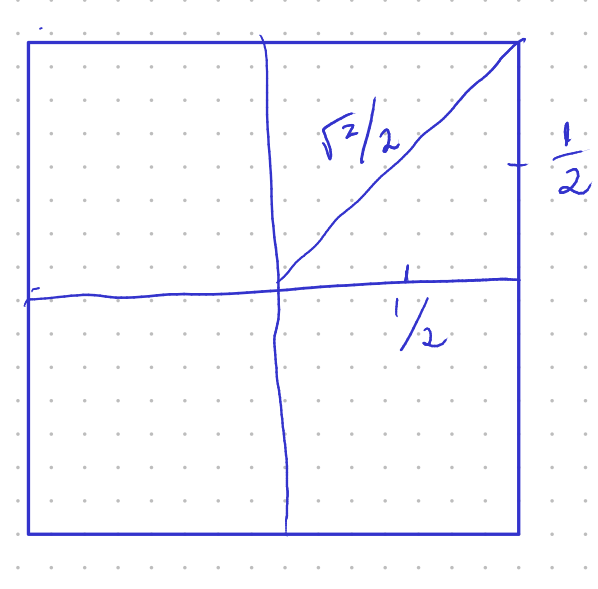
\includegraphics[width=0.5\textwidth]{images/12-03-04.png}
\end{figure}
\end{prooflist}

\begin{prooflist}{5. Prove that any set of seven distinct natural numbers
    contains a pair of numbers whose sum or difference is divisible by 10 .}
\item Let $A=\set{a_1, a_2, a_3, a_4, a_5, a_6, a_7\mid a_i\in\mathbb{N}}$, $|A|=7$.
\item Let $B=\set{\set{0}, \set{1, 9},\set{2, 8},\set{3, 7},\set{5}, \set{4, 6}}$,
    $|B|=6$.
\item Let $f=A\rightarrow B$ be the function from $A$ to $B$. Because $|A|>|B|$,
$f$ is not injective. The function $f$ takes a natural number $a$ and then maps
the value $a\mod 10=b$ to the element of $B$ which contains $b$. For example
$f(10)=\set{0}$, $f(41) = \set{1, 9}$, and $f(-18) = \set{2, 8}$.
Because $f$ is not injective, 2 elements $a_i, a_j\in A$ will map to the same element
in $B$. We now show that $10\mid a_i+a_j \lor 10\mid a_i-a_j$.
\item First we consider the case when $f(a_i) = f(a_j) \neq \set{0}$. Suppose
    $a_i = 10\cdot n + r$, where $r$ is the remainder after dividing by
    10 and $n$ is some integer. Similarly $a_j=10\cdot m + s$, where $s$ is the
    remainder and $m$ is some integer. Because of the way $B$ is defined,
    $m+n=10$.
\begin{align*}
    a_i =& 10\cdot n + r\\
    a_j =& 10\cdot m + s\\
    a_i + a_j =& 10\cdot n + r + 10\cdot m + s\\
    a_i + a_j =& 10(n + r) + m + s \\
    a_i + a_j =& 10(n + r) + 10 \\
    a_i + a_j =& 10(n + r + 1)
\end{align*}
Therefore $10\mid a_i + a_j$.
\item Now we consider the case when $f(a_i) = f(a_j)= \set{0}$. Then $10\mid a_i
    \land 10\mid a_j$.
\begin{align*}
    a_i =& 10\cdot n\\
    a_j =& 10\cdot m\\
    a_i + a_j =& 10\cdot n + 10\cdot m\\
    a_i + a_j =& 10(n + r)
\end{align*}
Therefore $10\mid a_i + a_j$.
\item Thus we have proven the following statement
\quote{Any set of seven distinct natural numbers
contains a pair of numbers whose sum or difference is divisible by 10.}
\end{prooflist}

\begin{prooflist}{6. Given a sphere $S$, a great circle of $S$ is the
    intersection of $S$ with a plane through its center. Every great circle
divides $S$ into two parts. A hemisphere is the union of the great circle and
one of these two parts. Prove that if five points are placed arbitrarily on $S$,
then there is a hemisphere that contains four of them.}
\item Select two of the five arbitrary points. With those two points and the
    center of the sphere, define a plane that bisects the sphere. The
    intersection of that plane and the sphere is a great circle $G$.
\item The remaining three points are placed in the two bisections defined by
    $G$. By the pigeonhole principle, one of those bisections $B_1$ has two of
    the remaining points.
\item A hemisphere is defined as the union of one of the bisections caused the
    by the great circle and the great circle itself. Therefore $H_1 = G \cup B_1$. $G$ has two points and
    $B_1$ has two points, therefore $H_1$ has four points.
\end{prooflist}

\begin{prooflist}{7. Prove or disprove: Any subset $X \subseteq\set{1,2,3, \ldots,
    2 n}$ with $|X|>n$ contains two (unequal) elements $a, b \in X$ for which
$a \mid b$ or $b \mid a$.}
\item Let $A=\set{1,2,3, \ldots, 2 n}$.
\item Let $X\subseteq A$ such that $|X|>n$.
\item Let $E(x)$ mean $x$ is even.
\item Let $O(x)$ mean $x$ is odd.
\item The set $A$ can be partitioned by parity---evens and odds.
\item Let $B=\set{x\in A \mid E(x)}$. Each $b\in B$ can be written as $b=2c$,
    for some integer $c\in A$.

\item Let $A_1=\set{1,2,3,4, 5, 6, 7, 8, 9, 10 }, n=5$.
\item Let $X_1=\set{1, 3, 5, 7, 9}, |X_1|=6$.

\item  Let us partition $A$ into two sets $B=\set{1\dots n}$ and
    $C=\set{n+1\dots 2n}$.
\item Each element of $C$ is either even or odd and can be written as either
    $2a$ or $2b+1$. For the even elements in $C$,
\item maybe partition into 4 sets?
\item Use the techniques from how to prove it.
\item To use the pigeonhole principle, devise a function that proves the point
    and is not injective
\item $f :: \mathbb{N} \rightarrow ? $
\item to linger upon ...
\end{prooflist}

\begin{prooflist}{7-2. Prove or disprove: Any subset $X \subseteq\set{1,2,3, \ldots,
    2 n}$ with $|X|>n$ contains two (unequal) elements $a, b \in X$ for which
$a \mid b$ or $b \mid a$.}
\item Let $A=\set{1,2,3, \ldots, 2 n}$.
\item Let $B=$ set of prime factors for a natural number $n$.
\item Let $X\subseteq A$ such that $|X|>n$.
\item Let $f=\mathbb{N} \rightarrow B $ be a function that takes a natural
    number and returns a set which contains sets as elements. The elemental-sets
    are organized such that
\item Example $f(9) = \set{3}$, $f(12) = \set{2, 2, 3}$.
\begin{align*}
    f(1) =& \set{1}\\
    f(2) =& \set{2}\\
    f(3) =& \set{3}\\
    f(4) =& \set{2}\\
    f(5) =& \set{5}\\
    f(6) =& \set{2, 3}\\
    f(7) =& \set{7}\\
    f(8) =& \set{2}\\
    f(9) =& \set{3}\\
    f(10) =& \set{2, 5}
\end{align*}
\end{prooflist}

\begin{prooflist}{7-3. Prove or disprove: Any subset $X \subseteq\set{1,2,3, \ldots,
    2 n}$ with $|X|>n$ contains two (unequal) elements $a, b \in X$ for which
$a \mid b$ or $b \mid a$.}
\item Let $A=\set{1,2,3, \ldots, 2 n}$.
\item Let $B=$ set of prime factors for a natural number $n$.
\item Let $X\subseteq A$ such that $|X|>n$.
\item Let $f=\mathbb{N} \rightarrow B $ be a function that takes a natural
    number and returns a set which contains sets as elements. The elemental-sets
    are organized such that
\item $f$ puts the element into a set with its highest factor if not prime.
\item $B=\set{\set{2, 4, 8, 16,\dots}, \set{3, 6, 9, \dots}, \set{5, 25, 625,
    \dots}}$.
\begin{align*}
    f(1) =& \set{1}\\
    f(2) =& \set{2}\\
    f(3) =& \set{3}\\
    f(4) =& \set{2}\\
    f(5) =& \set{5}\\
    f(6) =& \set{2, 3}\\
    f(7) =& \set{7}\\
    f(8) =& \set{2}\\
    f(9) =& \set{3}\\
    f(10) =& \set{2, 5}
\end{align*}
\end{prooflist}

\end{document}

\documentclass{hippoidC}

\memoto{Idris}
\memosubject{Book of Proof}
\memodate{2024.03.24}
\status{\S 12.4 Composition}

\begin{document}
\toc
\thispagestyle{styleTOC}
\pagebreak
\pagestyle{styleE}

\begin{prooflist}{1. Suppose $A=\{5,6,8\}, B=\{0,1\}, C=\{1,2,3\}$. Let $f: A
			\rightarrow B$ be the function $f=$ $\{(5,1),(6,0),(8,1)\}$, and $g: B
			\rightarrow C$ be $g=\{(0,1),(1,1)\}$. Find $g \circ f$.}
	\item $g \circ f = g(f(x)), \forall x\in A$
	\begin{align*}
		g \circ f(5) & = g(f(5)) = g(1) = 1 \\
		g \circ f(6) & = g(f(6)) =g(0) = 1  \\
		g \circ f(8) & = g(f(8)) =g(1) = 1  \\
	\end{align*}
	\item Therefore $g\circ f$ is the set $\set{(5, 1), (6, 1), (8, 1)}$.
\end{prooflist}

\begin{prooflist}{2. $g \circ f$.}
	\item $A=\{1,2,3,4\}$
	\item $B=\{0,1,2\}$
	\item $C=\{1,2,3\}$
	\item $f: A \rightarrow B$, $f=\{(1,0),(2,1)$, $(3,2),(4,0)\}$
	\item $g: B \rightarrow C$, $g=\{(0,1),(1,1),(2,3)\}$
	\item $g \circ f = g(f(x)), \forall x\in A$
	\begin{align*}
		g \circ f(1) & = g(f(1)) = g(0) = 1 \\
		g \circ f(2) & = g(f(2)) = g(1) = 1 \\
		g \circ f(3) & = g(f(3)) = g(2) = 3 \\
		g \circ f(4) & = g(f(4)) = g(0) = 1 \\
	\end{align*}
	\item Therefore $g\circ f$ is the set $\set{(1, 1), (2, 1), (3, 3), (4, 1)}$.
\end{prooflist}

\begin{prooflist}{3. Find $g \circ f$ and $f \circ g$.}
	\item
	$A=\{1,2,3\}$
	\item
	$f: A \rightarrow A$, $f=\{(1,2),(2,2),(3,1)\}$
	\item
	$g: A \rightarrow A$, $g=\{(1,3),(2,1),(3,2)\}$.
	\item $g \circ f = g(f(x)), \forall x\in A$
	\begin{align*}
		g \circ f(1) & = g(f(1)) = g(2) = 1 \\
		g \circ f(2) & = g(f(2)) = g(2) = 1 \\
		g \circ f(3) & = g(f(3)) = g(1) = 3
	\end{align*}
	\item Therefore $g\circ f$ is the set $\set{(1, 1), (2, 1), (1, 3)}$.
	\item $f \circ g = f(g(x)), \forall x\in A$
	\begin{align*}
		f \circ g(1) & = f(g(1)) = f(3) = 1 \\
		f \circ g(2) & = f(g(2)) = f(1) = 2 \\
		f \circ g(3) & = f(g(3)) = f(2) = 2
	\end{align*}
	\item Therefore $f\circ g$ is the set $\set{(1, 1), (2, 2), (3, 2)}$.
\end{prooflist}

\begin{prooflist}{4. Find $g \circ f$ and $f \circ g$.}
	\item $A=\set{a, b, c}$.
	\item $f: A \rightarrow A$ be the function $f=\{(a, c),(b, c),(c, c)\}$
	\item $g: A \rightarrow A$ be the function $g=\{(a, a),(b, b),(c, a)\}$.
	\item Find $g \circ f$ and $f \circ g$.
	\item $g \circ f = g(f(x)), \forall x\in A$
	\begin{align*}
		g \circ f(a) & = g(f(a)) = g(c) = a \\
		g \circ f(b) & = g(f(b)) = g(c) = a \\
		g \circ f(c) & = g(f(c)) = g(c) = a
	\end{align*}
	\item Therefore $g\circ f$ is the set $\set{(a, a), (b, a), (c, a)}$.
	\item $f \circ g = f(g(x)), \forall x\in A$
	\begin{align*}
		f \circ g(a) & = f(g(a)) = f(a) = c \\
		f \circ g(b) & = f(g(b)) = f(b) = c \\
		f \circ g(c) & = f(g(c)) = f(a) = c
	\end{align*}
	\item Therefore $f\circ g$ is the set $\set{(a, c), (b, c), (c, c)}$.
\end{prooflist}

\begin{prooflist}{5. Consider the functions $f, g: \mathbb{R} \rightarrow
			\mathbb{R}$ defined as $f(x)=\sqrt[3]{x+1}$ and $g(x)=x^3$. Find the
		formulas for $g \circ f$ and $f \circ g$.}
	\item $g \circ f = g(f(x)), \forall x\in \mathbb{R}$
	\begin{align*}
		g \circ f(x) = & g(f(x))                      \\
		=              & g\left(\sqrt[3]{x+1}\right)  \\
		=              & \left(\sqrt[3]{x+1}\right)^3 \\
		=              & x+1
	\end{align*}
	\item $f \circ g = f(g(x)), \forall x\in \mathbb{R}$
	\begin{align*}
		f \circ g(x) = & f(g(x))         \\
		=              & f(x^3)          \\
		=              & \sqrt[3]{x^3+1}
	\end{align*}
\end{prooflist}

\begin{prooflist}{6. Consider the functions $f, g: \mathbb{R} \rightarrow
			\mathbb{R}$ defined as $f(x)=\frac{1}{x^2+1}$ and $g(x)=3 x+2$. Find the
		formulas for $g \circ f$ and $f \circ g$.}
	\item $g \circ f = g(f(x)), \forall x\in \mathbb{R}$
	\begin{align*}
		g \circ f = & g(f(x))                           \\
		=           & g\left(\frac{1}{x^2+1}\right)     \\
		=           & 3\left(\frac{1}{x^2+1}\right) + 2 \\
		=           & \frac{3}{x^2+1} + 2               \\
	\end{align*}
	\item $f \circ g = f(g(x)), \forall x\in \mathbb{R}$
	\begin{align*}
		f \circ g = & f(g(x))                \\
		=           & f(3x^2+1)              \\
		=           & \frac{1}{(3x^2+1)^2+1} \\
	\end{align*}
\end{prooflist}

\begin{prooflist}{7. Consider the functions $f, g: \mathbb{Z} \times \mathbb{Z}
			\rightarrow \mathbb{Z} \times \mathbb{Z}$ defined as $f(m, n)=(m n,
			m^2)$ and $g(m, n)=(m+1, m+n)$. Find the formulas for $g \circ f$
		and $f
			\circ g$.}
	\item $g \circ f = g(f((m, n))), \forall (m, n)\in \mathbb{Z}\times\mathbb{Z}$
	\begin{align*}
		g \circ f = & g(f((m, n)))               \\
		=           & g\left( (m n, m^2) \right) \\
		=           & (mn + 1, mn + m^2)
	\end{align*}
	\item $f \circ g = f(g((m, n))), \forall (m, n)\in \mathbb{Z}\times\mathbb{Z}$
	\begin{align*}
		f \circ g = & f(g((m, n)))         \\
		=           & f((m+1, m + n))      \\
		=           & ((m+1)(m+n),(m+1)^2)
	\end{align*}
\end{prooflist}

\begin{prooflist}{8. Consider the functions $f, g: \mathbb{Z} \times \mathbb{Z}
			\rightarrow \mathbb{Z} \times \mathbb{Z}$ defined as $f(m, n)=(3 m-4 n, 2
			m+n)$ and $g(m, n)=(5 m+n, m)$. Find the formulas for $g \circ f$ and $f \circ
			g$.}
	\item $g \circ f = g(f((m, n))), \forall (m, n)\in \mathbb{Z}\times\mathbb{Z}$
	\begin{align*}
		g \circ f = & g(f((m, n)))                  \\
		=           & g\left( (3m-4n, 2m+n) \right) \\
		=           & (5(3m-4n) + 2m+n, 3m-4n)      \\
		=           & (15m-20n+ 2m+n, 3m-4n)        \\
		=           & (17m-19n, 3m-4n)
	\end{align*}
	\item $f \circ g = f(g((m, n))), \forall (m, n)\in \mathbb{Z}\times\mathbb{Z}$
	\begin{align*}
		f \circ g = & f(g((m, n)))                \\
		=           & f((5m+n, m))                \\
		=           & (3(5m+n) - 4m, 2(5m+n) + m) \\
		=           & (11m+3n, 11m+2n)
	\end{align*}
\end{prooflist}

\begin{prooflist}{9. Consider the functions $f: \mathbb{Z} \times \mathbb{Z}
			\rightarrow \mathbb{Z}$ defined as $f(m, n)=m+n$ and $g: \mathbb{Z}
			\rightarrow \mathbb{Z} \times \mathbb{Z}$ defined as $g(m)=(m, m)$. Find the
		formulas for $g \circ f$ and $f \circ g$.}
	\item $g \circ f = g(f((m, n))), \forall (m, n)\in \mathbb{Z}\times\mathbb{Z}$
	\begin{align*}
		g \circ f = & g(f((m, n))) \\
		=           & g(m+n )      \\
		=           & (m+n, m+n)
	\end{align*}
	\item $f \circ g = f(g(m)), \forall m\in \mathbb{Z}$
	\begin{align*}
		f \circ g = & f(g(m))   \\
		=           & f((m, m)) \\
		=           & 2m
	\end{align*}

\end{prooflist}

\begin{prooflist}{10. Consider the function $f: \mathbb{R}^2 \rightarrow
			\mathbb{R}^2$ defined by the formula $f(x, y)=\left(x y, x^3\right)$. Find a
		formula for $f \circ f$.}
	\item $f \circ f = f(f((x, y))), \forall , (x, y)\in \mathbb{R}^2$.
	\begin{align*}
		f \circ f = & f(f((x, y)))  \\
		=           & f((xy, x^3) ) \\
		=           & (x^4y, x^9)
	\end{align*}
\end{prooflist}

\end{document}

\documentclass{hippoidC}

\memoto{Idris}
\memosubject{Book of Proof}
\memodate{2024.03.24}
\status{\S 12.5 Inverse}

\begin{document}
\toc
\thispagestyle{styleTOC}
\pagebreak
\pagestyle{styleE}

\begin{prooflist}{1. Check that $f: \mathbb{Z} \rightarrow \mathbb{Z}$ defined
    by $f(n)=6-n$ is bijective. Then compute $f^{-1}$.}
\inj{}
\item Suppose some $a, b \in \mathbb{Z}$ and that $f(a) = f(b)$.
\begin{align*}
    f(a)&=f(b)\\
    6-a&=6-b\\
    a&=b
\end{align*}
Therefore we have proved the contrapositive of the injective implication and $f$
is injective.
\surj{}
\item Suppose some $b\in \mathbb{Z}$.
\begin{align*}
    b&=f(a)\\
    b&=6-a\\
    b-6&=-a\\
    6-b&=a
\end{align*}
Therefore we have shown that there exists an $a\in\mathbb{Z}$ such that $f(a)=b$
for all $b$, therefore $f$ is surjective. Since $f$ is surjective and injective
it is also bijective. Because $f$ is bijective, it's inverse $f^{-1}$ does exist
such that $a=f\circ f^{-1}(a)$.
\begin{align*}
    f(x)=y=&6-x\\
    x=&6-y&&\text{swap x and y to get to }f^{-1}\\
    x-6=&-y\\
    6-x=&y\\
    f^{-1}(x)=&6-x
\end{align*}
\end{prooflist}

\begin{prooflist}{2. In Exercise 9 of Section 12.2 you proved that $f:
    \mathbb{R}-\{2\} \rightarrow \mathbb{R}-\{5\}$ defined by $f(x)=\frac{5
x+1}{x-2}$ is bijective. Now find its inverse.}
\item
\begin{align*}
    f(x)=y=&\frac{5 x+1}{x-2}\\
    x=&\frac{5y+1}{y-2}&&\text{swap x and y to get to }f^{-1}\\
    (y-2)x=&5y+1\\
    yx-2x=&5y+1\\
    -2x-1=&5y-yx\\
    -2x-1=&y(5-x)\\
    \frac{-2x-1}{5-x}=&y\\
    f^{-1}(x) =& \frac{-2x-1}{5-x}
\end{align*}
\end{prooflist}

\begin{prooflist}{3. Let $B=\left\{2^n: n \in \mathbb{Z}\right\}=\left\{\ldots,
    \frac{1}{4}, \frac{1}{2}, 1,2,4,8, \ldots\right\}$. Show that the function
$f: \mathbb{Z} \rightarrow B$ defined as $f(n)=2^n$ is bijective. Then find
$f^{-1}$.}
\inj{}
\begin{align*}
    f(a)&=f(b)\\
    2^a&=2^b\\
    \log 2^a&=\log 2^b\\
    a \log 2&=b \log 2\\
    a&=b
\end{align*}
\surj{}
\begin{align*}
    b&=f(a)\\
    b&=2^a\\
    \log b&=a \log 2\\
    \frac{\log b}{\log 2} &= a\\
    \frac{b}{2} &= a\\
    \frac{b}{2} &= a\\
\end{align*}
Therefore $f$ is surjective and injective.
\begin{align*}
    f(x)=y=&2^x\\
    x=&2^y&&\text{swap x and y to get to }f^{-1}\\
    \log_2 x=&\log_2 2^y\\
    \log_2 x=&y\\
    f^{-1}(x) =& \log_2 x
\end{align*}
\end{prooflist}

\begin{prooflist}{4. The function $f: \mathbb{R} \rightarrow(0, \infty)$ defined
    as $f(x)=e^{x^3+1}$ is bijective. Find its inverse.}
    \item
\begin{align*}
    f(x)=y=&e^{x^3+1}\\
    x=&e^{y^3+1}&&\text{swap x and y to get to }f^{-1}\\
    \ln x=&\ln e^{y^3+1}\\
    \ln x=&y^3+1\\
    \ln x-1=&y^3\\
    \sqrt[3]{\ln x-1}=&y\\
    f^{-1}(x) =& \sqrt[3]{\ln x-1}
\end{align*}
\end{prooflist}

\begin{prooflist}{5. The function $f: \mathbb{R} \rightarrow \mathbb{R}$ defined
    as $f(x)=\pi x-e$ is bijective. Find its inverse.}
\item
\begin{align*}
    f(x)=y=&\pi x-e\\
    x=&\pi y-e&&\text{swap x and y to get to }f^{-1}\\
    x+e=&\pi y\\
    \frac{x+e}{\pi}=&y\\
    f^{-1}(x) =& \frac{x+e}{\pi}
\end{align*}
\end{prooflist}

\begin{prooflist}{6. The function $f: \mathbb{Z} \times \mathbb{Z} \rightarrow
    \mathbb{Z} \times \mathbb{Z}$ defined by the formula $f(m, n)=(5 m+4 n, 4
m+3 n)$ is bijective. Find its inverse.}
\item
\begin{align*}
    f(m, n)=(j, k)=&(5 m+4 n, 4 m+3 n)\\
    (m, n)=&(5 j+4 k, 4 j+3 k)&&\text{swap m,n and j,k to get to }f^{-1}\\
    m=&5 j+4 k\\
    n=&4 j+3 k\\
    3m=&15 j+12 k\\
    4n=&16 j+12 k\\
    3m-4n=&-j\\
    4n-3m=&j\\
    4n=&16 (4n-3m)+12 k\\
    4n=&64n-48m+12 k\\
    48m-60n=&12 k\\
    4m-5n=&k\\
    f^{-1}(m, n) =& (4n-3m, 4m-5n)
\end{align*}
\end{prooflist}

\begin{prooflist}{7. Show that the function $f: \mathbb{R}^2 \rightarrow
    \mathbb{R}^2$ defined by the formula $f(x, y)=\left(\left(x^2+1\right) y,
x^3\right)$ is bijective. Then find its inverse.}
\inj{}
\begin{align*}
    f(a, b)&=f(c, d)\\
    \left(\left(a^2+1\right)b, a^3\right)&= \left(\left(c^2+1\right)d, c^3\right)\\
    a^3&=c^3\\
    a&=c\\
    (a^2+1)b &= (c^2+1)d\\
    (a^2+1)b &= (a^2+1)d\\
    b &= d
\end{align*}
Therefore we have shown that $f$ is injective by proving the injective
implication contrapositive.
\surj{}
\begin{align*}
    (c, d) &= f(a, b)\\
    (c, d) &= \left(\left(a^2+1\right)b, a^3\right)\\
    a^3&=d\\
    a&=\sqrt[3]{d}\\
    (a^2+1)b&=c\\
    b&=\dfrac{c}{a^2+1}\\
    b&=\dfrac{c}{d^{\frac{2}{3}}+1}
\end{align*}
Therefore we have shown that $f$ is surjective by showing that for any arbitrary
$(c, d)$ in the codomain, we can find an $(a, b)$ in the domain such that $f(a,
b)=(c, d)$.
\item We can re-use the calculations from the surjetive proof to determine the inverse
$f^{-1}(a, b)$.
\[f^{-1}(x, y) = \left(\dfrac{x}{y^{\frac{2}{3}}+1}, \sqrt[3]{x}\right)
\]
\end{prooflist}

\begin{prooflist}{8. Is the function $\theta: \mathscr{P}(\mathbb{Z})
    \rightarrow \mathscr{P}(\mathbb{Z})$ defined as $\theta(X)=\bar{X}$
bijective? If so, find $\theta^{-1}$.}
\item
\inj{}
\begin{align*}
    \theta(X)&=\theta(Y)\\
    \overline{X}&=\overline{Y}\\
\end{align*}
If two sets are equal, they're the same set. Therefore $\theta$ is injective.
\surj{}
\begin{align*}
    \theta(X)&=Y\\
    \overline{X}&=Y\\
    X&=\overline{Y}\\
\end{align*}
For any value in the $Y$ codomain, we can find a value $X$ in the domain such
that $\theta{X}=Y$, therefore $\theta$ is injective, surjective, and bijective.
To find the inverse, note that $\theta$ takes a set $X$, and subtracts it from
the universe of $U=\mathbb{Z}$, such that $\theta(X)=U-X$. To do the inverse, we
must subtract that from the universe such that $\theta^{-1}=U-(U-X)=X$.
\end{prooflist}

\begin{prooflist}{9. Consider the function $f: \mathbb{R} \times \mathbb{N}
    \rightarrow \mathbb{N} \times \mathbb{R}$ defined as $f(x, y)=(y, 3 x y)$.
Check that this is bijective; find its inverse.}
\item nah, i get it.
\end{prooflist}

\begin{prooflist}{10. Consider $f: \mathbb{N} \rightarrow \mathbb{Z}$ defined as
    $f(n)=\frac{(-1)^n(2 n-1)+1}{4}$. This function is bijective by Exercise 18
in Section 12.2. Find its inverse.}
\item nah, i get it.
\end{prooflist}

\end{document}

\documentclass{article}
\makeindex

\usepackage{amsmath}
\usepackage{amssymb}
\usepackage{booktabs}
\usepackage{csvsimple-l3}
\usepackage{bussproofs}
\usepackage{dirtytalk}
\usepackage[dvipsnames]{xcolor}
\usepackage{enumitem}
\usepackage{epigraph}
\usepackage{forest}
\usepackage{formal-grammar}
\usepackage{graphicx}
\usepackage[citecolor=blue,colorlinks=true, linkcolor=blue, urlcolor=blue]{hyperref}
\usepackage{kantlipsum}
\usepackage{makeidx}
\usepackage[margin=0.8in]{geometry}
\usepackage{mathrsfs}
\usepackage[outputdir=../build]{minted}
\usepackage{multicol}
\usepackage[mode=tex]{standalone}
\usepackage[style=authortitle]{biblatex}
\usepackage[T1]{fontenc}
\usepackage[tableaux]{prooftrees}
\usepackage{tcolorbox}
\usepackage{tikz}
\usepackage{titlesec}
\usepackage{xcolor}

\usetikzlibrary{arrows}
\usetikzlibrary{arrows.meta}
\usetikzlibrary{automata}
\usetikzlibrary{calc}
\usetikzlibrary{fit}
\usetikzlibrary{petri}
\usetikzlibrary{positioning}

\tcbuselibrary{breakable}
\tcbuselibrary{listings}
\tcbuselibrary{minted}
\tcbuselibrary{skins}
\tcbuselibrary{theorems}

\newcounter{filePrg}

\addbibresource{biblio.bib}
\setlength{\parindent}{0pt}

\renewcommand{\emph}[1]{\textit{#1}}
\setlength{\parindent}{0pt}

\newcommand\setboxcounter[2]{\setcounter{tcb@cnt@#1}{#2}}
\newcommand\qed[0]{\blacksquare}
\setlength{\parindent}{10pt}
\newcommand{\set}[1]{\{#1\}}
\newcommand{\up}[1]{ \left\lceil#1\right\rceil }
\newcommand{\down}[1]{ \left\lfloor#1\right\rfloor}

\definecolor{CaribbeanBlue}{RGB}{0, 206, 209} % Define Caribbean Blue
\NewTcbTheorem[list inside=definition]{definition}
{Definition}{
	breakable,
	colback=CaribbeanBlue!05,
	colframe=CaribbeanBlue!35!black,
	fonttitle=\bfseries}{th}

\NewTcbTheorem[list inside=intuition]{intuition}{Intuition}{
	breakable,
	colback=blue!5,
	colframe=blue!35!black,
	fonttitle=\bfseries}{th}

\NewTcbTheorem{example}{Example}{
	breakable,
	colback=white,
	colframe=green!35!black,
	fonttitle=\bfseries}{th}

\NewTcbTheorem{verify}{Verify}{
	breakable,
	float,
	colback=red!5,
	colframe=red!35!black,
	fonttitle=\bfseries}{th}

\NewTcbTheorem[list inside=theorem]{theorem}{Theorem}{
	breakable,
	colback=gray!10,
	colframe=gray!35!black,
	fonttitle=\bfseries}{th}

% \NewTcbTheorem[
% list inside=exercise,
% number within=chapter,
% number within=section,
% ]

\NewTcbTheorem[
	list inside=exercise,
	number within=section,
]{exercise}{Exercise}{
	breakable,
	colback=white,
	colframe=black,
	fonttitle=\bfseries}{th}

\newcommand{\hask}[1]{\mintinline{haskell}{#1}}

\newenvironment{alist}
{\begin{enumerate}[label={*}, leftmargin=*, itemsep=0pt, parsep=0pt]}
		{\end{enumerate}}

\newenvironment{blist}
{\begin{enumerate}[label={}, leftmargin=*, itemsep=0pt, parsep=0pt]}
		{\end{enumerate}}

\renewcommand{\thesection}{\arabic{section}}
\tcbset{enhanced jigsaw}

\newtcbinputlisting{\codeFromFile}[2]{
	listing file={#1},
	listing engine=minted,
	minted style=colorful,
	minted language=haskell,
	minted options={breaklines,linenos,numbersep=3mm},
	colback=blue!5!white,colframe=blue!75!black,listing only,
	left=5mm,enhanced,
	title={#2},
	overlay={\begin{tcbclipinterior}\fill[red!20!blue!20!white] (frame.south west)
				rectangle ([xshift=5mm]frame.north west);\end{tcbclipinterior}}
}

\newtcblisting{haskell}[1]
{
	listing engine=minted,
	minted style=colorful,
	minted language=haskell,
	minted options={breaklines,linenos,numbersep=3mm},
	colback=blue!5!white,colframe=blue!75!black,listing only,
	left=5mm,enhanced,
	title={#1},
	overlay={\begin{tcbclipinterior}\fill[red!20!blue!20!white] (frame.south west)
				rectangle ([xshift=5mm]frame.north west);\end{tcbclipinterior}}
}


\begin{document}
\section{Image and Preimage}

\begin{exercise}{}{}
	{1. Consider the function $f: \mathbb{R} \rightarrow \mathbb{R}$ defined as
		$f(x)=x^2+3$. Find $f([-3,5])$ and $f^{-1}([12,19])$.}
	\begin{alist}
		% \item \imagedef{}
		\item Let $X\subset \mathbb{R}= [-3,5]$. $f(X)$ is a image of the function $f$.
		\item Let $Y\subset \mathbb{R}= [12,19]$. $f^{-1}(Y)$ is a preimage of the
		function $f^{-1}$.
	\end{alist}
	Let's determine $f^{-1}$ to calculate the preimage.
	\begin{align*}
		f(x) = y = & x^2+3                                                   \\
		x=         & y^2+3         &  & \text{swap x and y to get to }f^{-1} \\
		y^2=       & x-3                                                     \\
		y=         & \pm\sqrt{x-3}
	\end{align*}
	\begin{align*}
		f(X) =      & f([-3, 5]) = [12, 28]                   \\
		f^{-1}(Y) = & f^{-1}([12, 19]) = [-3, -5] \cup [3, 5]
	\end{align*}
\end{exercise}{}{}


\begin{exercise}{}{}
	{2. Consider the function $f:\{1,2,3,4,5,6,7\} \rightarrow\{0,1,2,3,4,5,6,7,8,9\}$ }
	% \imagedef{}
	\begin{align*}
		f=\set{(1,3),(2,8),(3,3),(4,1),(5,2),(6,4),(7,6)}
	\end{align*}
	Find:
	\begin{align*}
		f(\set{1,2,3})=         & \set {3, 8}      \\
		f(\set{4,5,6,7}) =      & \set{1, 2, 4, 6} \\
		f(\varnothing) =        & \set{}           \\
		f^{-1}(\set{0,5,9}) =   & \set{}           \\
		f^{-1}(\set{0,3,5,9}) = & \set{3}          \\
	\end{align*}
\end{exercise}{}{}

\begin{exercise}{}{}
	{3. This problem concerns functions $f:\{1,2,3,4,5,6,7\}
			\rightarrow\{0,1,2,3,4\}$. How many such functions have the property that
		$\left|f^{-1}(\{3\})\right|=3$ ?}
	\begin{alist}
		\item Let $A:\set{1,2,3,4,5,6,7}$
		\item Let $B:\set{0,1,2,3,4}$
		\item $f:A\rightarrow B$
		\item In words, this question is asking how many functions $f$ have a preimage
		such that the input set $\set{3}$ has a cardinality 3.
		\item This means that 3 values in the domain of $f$ map to 3 in the codomain.
		For the function $f$, we must map each value in $A$ to some value in $B$, 7
		choices total.  We must pick 3 choices to go to 3, which is counted as
		$\binom{7}{3}$. The remaining 4 values can map to any value but 3, therefore
		$4^4$.
		\item Using the multiplication principle, we calculate the cardinality of $f$ as
		$\binom{7}{3}\cdot 4^4$.
	\end{alist}
\end{exercise}{}{}

\begin{exercise}{}{}
	{4. This problem concerns functions $f:\{1,2,3,4,5,6,7,8\}
			\rightarrow\{0,1,2,3,4,5,6\}$. How many such functions have the property
		that $\left|f^{-1}(\{2\})\right|=4$ ?}
	\begin{alist}
		\item Let $A:\set{1,2,3,4,5,6,7, 8}$
		\item Let $B:\set{0,1,2,3,4, 5, 6}$
		\item $f:A\rightarrow B$
		\item In words, this question is asking how many functions $f$ have a preimage
		such that the input set $\set{2}$ has a cardinality 4.
		\item This means that 4 values in the domain of $f$ map to 2 in the codomain.
		For the function $f$, we must map each value in $A$ to some value in $B$, 8
		choices total.  We must pick 4 choices to go to 2, which is counted as
		$\binom{8}{4}$. The remaining 4 values can map to any value but 2, therefore
		$4^6$.
		\item Using the multiplication principle, we calculate the cardinality of $f$ as
		$\binom{8}{4}\cdot 4^6$.
	\end{alist}
\end{exercise}{}{}

\begin{exercise}{}{}
	{5. Consider a function $f: A \rightarrow B$ and a subset $X
			\subseteq A$. We observed in Example 12.14 that $f^{-1}(f(X)) \neq X$ in
		general. However $X \subseteq f^{-1}(f(X))$ is always true. Prove this.}
	\begin{alist}
		% \item \imagedef{}
		\item Let $x$ be in $X$. Then $f(x) \in f(X)$. By definition $f^{-1}(f(x))$ is in
		$X$. Therefore we have shown that if $x\in X$, then $x\in f^{-1}(f(X))$.
		\item Thus we have shown that $X \subseteq f^{-1}(f(X))$
	\end{alist}
\end{exercise}{}{}

\begin{exercise}{}{}
	{6. Given a function $f: A \rightarrow B$ and a subset $Y
			\subseteq B$, is $f\left(f^{-1}(Y)\right)=Y$ always true? Prove or give a
		counterexample.}
	\begin{alist}
		% \item \imagedef{}
		\item In general $f\left(f^{-1}(Y)\right)=Y$ is not true. For any function $f$
		which is not bijective, the statement will be false. Let us now construct
		such a non-bijective function as a counterexample.
		\item Let $A=\set{1, 2, 3}$.
		\item Let $B=\set{a, b, c}$.
		\item Let $Y\subseteq B = \set{c}$.
		\item Let $f: A \rightarrow B$.
		\item Let $f = \set{(1, a), (2, a), (3, b)}$.
	\end{alist}
	\begin{align*}
		f\left(f^{-1}(Y)\right) & = f\left(f^{-1}(\set{c})\right) \\
		                        & = f(\varnothing)                \\
		                        & = \varnothing                   \\
		                        & \neq Y
	\end{align*}
\end{exercise}{}{}

\begin{exercise}{}{}
	{7. Given a function $f: A \rightarrow B$ and subsets $W, X \subseteq A$, prove $f(W \cap X) \subseteq f(W) \cap f(X)$.}
	% \imagedef{}
	\begin{align*}
		b\in f(W\cap X)                   &  & \text{supposition}           \\
		b\in \set{f(x): x \in W\cap X}    &  & \text{def.\ of image}        \\
		f(a) = b                          &  & \text{for some }a\in W\cap X \\
		a \in W \land a \in X             &  & \text{def.\ of image}        \\
		f(a) \in f(W) \land f(a) \in f(X) &  & \text{application of }f      \\
		f(W) \cap f(X)                    &  & \text{def.\ of }\cap
	\end{align*}
\end{exercise}{}{}

\begin{exercise}{}{}
	{8. Given a function $f: A \rightarrow B$ and subsets $W, X \subseteq A$,
		then $f(W \cap X)=f(W) \cap f(X)$ is false in general. Produce a
		counterexample.}
	% \imagedef{}
	\begin{align}
		f(W \cap X)=             & f(W) \cap f(X) &  & \text{false in general} \\
		f(W \cap X)\subseteq     & f(W) \cap f(X)                              \\
		f(W) \cap f(X) \subseteq & f(W \cap X)
	\end{align}
	For (1) to be true, (2) and (3) must be true. We have proven (2) to be true in
	the previous exercise, therefore there must be a counterexample for (3).
	\begin{alist}
		\item Let $A=\set{1, 2, 3, 4}$.
		\item Let $B=\set{a, b, c}$.
		\item Let $W\subseteq A = \set{1, 2, 3}$.
		\item Let $X\subseteq A = \set{2, 3, 4}$.
		\item Let $f: A \rightarrow B$.
		\item Let $f = \set{(1, a), (2, b), (3, c), (4, a)}$.
	\end{alist}
	\begin{align*}
		f(W) \cap f(X) \subseteq                         & f(W \cap X)                                              \\
		f(\set{1, 2, 3}) \cap f(\set{2, 3, 4}) \subseteq & f(\set{1, 2, 3} \cap \set{2, 3, 4})                      \\
		f(\set{1, 2, 3}) \cap f(\set{2, 3, 4}) \subseteq & f(\set{2, 3})                                            \\
		\set{a, b, c} \cap \set{b, c, a} \subseteq       & \set{b, c}                                               \\
		\set{a, b, c} \not\subseteq                      & \set{b, c}                          &  & \text{disproof}
	\end{align*}
\end{exercise}{}{}

\begin{exercise}{}{}
	{9. Given a function $f: A \rightarrow B$ and subsets $W, X
			\subseteq A$, prove $f(W \cup X)=f(W) \cup f(X)$.}
	% \imagedef{}
	\setcounter{equation}{0}
	\begin{align}
		f(W \cup X)=             & f(W) \cup f(X) \\
		f(W \cup X)\subseteq     & f(W) \cup f(X) \\
		f(W) \cup f(X) \subseteq & f(W \cup X)
	\end{align}
	For (1) to be true, (2) and (3) must be true. We'll start with (2).
	\begin{align}
		b\in                & f(W\cup X)                & \text{supposition}           \\
		b\in                & \set{f(x): x \in W\cup X} & \text{def.\ of image}        \\
		f(a) =              & b                         & \text{for some }a\in W\cup X \\
		a \in W \cup        & X                         & \text{def.\ of image}        \\
		a \in W \lor        & a \in X                   & \text{def.\ of image}        \\
		f(a) \in f(W) \lor  & f(a) \in f(X)             & \text{application of }f      \\
		f(a) \in (f(W) \cup & f(X))                     & \text{def.\ of }\lor         \\
		f(W) \cup           & f(X)                      & \text{def.\ of }\in
	\end{align}
	Thus we have shown (2). Now we will show (3).
	\begin{align}
		b\in f(W)\cup                 & b\in f(X)                & \text{supposition}                \\
		b\in \set{f(x): x \in W} \lor & b\in \set{f(x): x \in X} & \text{def.\ of image}             \\
		f(a) =                        & b                        & \text{for some }a\in W\lor a\in X \\
		a \in                         & W \lor a \in X           & \text{def.\ of image}             \\
		a \in                         & W \cup X                 & \text{def.\ of }\cup              \\
		f(a) \in                      & f(W\cup X)               & \text{application of }f           \\
		                              & f(W\cup X)               & \text{def.\ of }\in
	\end{align}
	Thus we have shown (2) and (3) and proven that
	\[
		f(W \cup X)=f(W) \cup f(X)
	\]
\end{exercise}{}{}

\begin{exercise}{}{}
	{10. Given $f: A \rightarrow B$ and subsets $Y, Z \subseteq B$, prove
		$f^{-1}(Y \cap Z)=f^{-1}(Y) \cap f^{-1}(Z)$.}
	% \imagedef{}
	\setcounter{equation}{0}
	\begin{align}
		f^{-1}(Y \cap Z)=                  & f^{-1}(Y) \cap f^{-1}(Z) \\
		f^{-1}(Y \cap Z)\subseteq          & f^{-1}(Y) \cap f^{-1}(Z) \\
		f^{-1}(Y) \cap f^{-1}(Z) \subseteq & f^{-1}(Y \cap Z)
	\end{align}
	For (1) to be true, (2) and (3) must be true. We'll start with (2).
	% \begin{align*}
	% a\in                          & f^{-1}(Y\cap Z)                 & \text{supposition}           \\
	% a\in                          & \set{x \in A: f(x) \in Y\cap Z} & \text{def.                   \\ of preimage}     \\
	% f^{-1}(b) =                   & a                               & \text{for some }b\in Y\cap Z \\
	% b \in Y \cap                  & Z                               & \text{def.                   \\ of preimage}     \\
	% b \in Y \land                 & b \in Z                         & \text{def.                   \\ of preimage}     \\
	% f^{-1}(b) \in f^{-1}(Y) \land & f^{-1}(b) \in f^{-1}(Z)         & \text{application of }f^{-1} \\
	% f^{-1}(Y) \cap                & f^{-1}(Z)                       & \text{def.                   \\ of }\cap
	% \end{align*}
	Thus we have shown (2). Now we will show (3).

	\begin{align}
		a\in f^{-1}(Y) \cap                  & f^{-1}(Z)                      & \text{supposition}                        \\
		a\in \set{x \in A: f(x) \in Y} \land & a\in \set{x \in A: f(x) \in Z} & \text{def.                   of preimage} \\
		a\in \set{x \in A: f(x)              & \in Y\cap Z}                   & \text{def.                   of }\cap     \\
		f^{-1}(b) = a                        &                                & \text{for some }b\in Y\cap Z              \\
		b \in                                & Y \cap Z                       & \text{def.                   of preimage} \\
		f^{-1}(b) \in                        & f^{-1}(Y\cap Z)                & \text{application of }f^{-1}              \\
		f^{-1}(Y\cap Z)                      &                                & \text{def.                   of }\in
	\end{align}
	Thus we have shown (2) and (3) and proven that
	\[
		f^{-1}(Y \cap Z)=f^{-1}(Y) \cap f^{-1}(Z)
	\]
\end{exercise}{}{}

\begin{exercise}{}{}
	{11. Given $f: A \rightarrow B$ and subsets $Y, Z \subseteq B$, prove
		$f^{-1}(Y \cup Z)=f^{-1}(Y) \cup f^{-1}(Z)$.}
	% \imagedef{}
	\setcounter{equation}{0}
	\begin{align}
		f^{-1}(Y \cup Z)=                  & f^{-1}(Y) \cup f^{-1}(Z) \\
		f^{-1}(Y \cup Z)\subseteq          & f^{-1}(Y) \cup f^{-1}(Z) \\
		f^{-1}(Y) \cup f^{-1}(Z) \subseteq & f^{-1}(Y \cup Z)
	\end{align}
	For (1) to be true, (2) and (3) must be true. We'll start with (2).
	\begin{align}
		a\in                         & f^{-1}(Y\cup Z)                 & \text{supposition}           \\
		a\in                         & \set{x \in A: f(x) \in Y\cup Z} & \text{def. of preimage}      \\
		f^{-1}(b) =                  & a                               & \text{for some }b\in Y\cup Z \\
		b \in Y \cup                 & Z                               & \text{def. of preimage}      \\
		b \in Y \lor                 & b \in Z                         & \text{def. of }\lor          \\
		f^{-1}(b) \in f^{-1}(Y) \lor & f^{-1}(b) \in f^{-1}(Z)         & \text{application of }f^{-1} \\
		f^{-1}(Y) \cup               & f^{-1}(Z)                       & \text{def. of }\cup
	\end{align}
	Thus we have shown (2). Now we will show (3).
	\begin{align}
		a\in f^{-1}(Y) \cup                 & f^{-1}(Z)                      & \text{supposition}           \\
		a\in \set{x \in A: f(x) \in Y} \lor & a\in \set{x \in A: f(x) \in Z} & \text{def. of preimage}      \\
		a\in \set{x \in A: f(x)             & \in Y\cup Z}                   & \text{def. of }\cup          \\
		f^{-1}(b) = a                       &                                & \text{for some }b\in Y\cup Z \\
		b \in                               & Y \cup Z                       & \text{def. of preimage}      \\
		f^{-1}(b) \in                       & f^{-1}(Y\cup Z)                & \text{application of }f^{-1} \\
		f^{-1}(Y\cup Z)                     &                                & \text{def. of }\in
	\end{align}
	Thus we have shown (2) and (3) and proven that
	\[
		f^{-1}(Y \cup Z)=f^{-1}(Y) \cup f^{-1}(Z)
	\]
\end{exercise}{}{}

\begin{exercise}{}{}
	{12. Consider $f: A \rightarrow B$. Prove that $f$ is injective if and only
		if $X=f^{-1}(f(X))$ for all $X \subseteq A$. Prove that $f$ is surjective if
		and only if $f\left(f^{-1}(Y)\right)=Y$ for all $Y \subseteq B$.}
	% \imagedef{}
	% \inj{}
	% \surj{}
\end{exercise}{}{}

\begin{exercise}{}{}
	{13. Let $f: A \rightarrow B$ be a function, and $X \subseteq A$. Prove or
		disprove: $f\left(f^{-1}(f(X))\right)=f(X)$.}
	\begin{alist}
		\item Probably it's false. It's using $f\circ f^{-1}$ as an identity, which
		doesn't hold unless you know $f$ is bijective, which is not provided.
	\end{alist}
\end{exercise}{}{}

\begin{exercise}{}{}
	{14. Let $f: A \rightarrow B$ be a function, and $Y \subseteq B$. Prove or
		disprove: $f^{-1}\left(f\left(f^{-1}(Y)\right)\right)=f^{-1}(Y)$.}
	\begin{alist}
		\item Probably it's false. It's using $f\circ f^{-1}$ as an identity, which
		doesn't hold unless you know $f$ is bijective, which is not provided.
		\item No it's true for some reason.
	\end{alist}
\end{exercise}{}{}

\end{document}


\printbibliography{}
\printindex{}
\end{document}
